\documentclass[twoside]{book}

% Packages required by doxygen
\usepackage{fixltx2e}
\usepackage{calc}
\usepackage{doxygen}
\usepackage[export]{adjustbox} % also loads graphicx
\usepackage{graphicx}
\usepackage[utf8]{inputenc}
\usepackage{makeidx}
\usepackage{multicol}
\usepackage{multirow}
\PassOptionsToPackage{warn}{textcomp}
\usepackage{textcomp}
\usepackage[nointegrals]{wasysym}
\usepackage[table]{xcolor}

% Font selection
\usepackage[T1]{fontenc}
\usepackage[scaled=.90]{helvet}
\usepackage{courier}
\usepackage{amssymb}
\usepackage{sectsty}
\renewcommand{\familydefault}{\sfdefault}
\allsectionsfont{%
  \fontseries{bc}\selectfont%
  \color{darkgray}%
}
\renewcommand{\DoxyLabelFont}{%
  \fontseries{bc}\selectfont%
  \color{darkgray}%
}
\newcommand{\+}{\discretionary{\mbox{\scriptsize$\hookleftarrow$}}{}{}}

% Page & text layout
\usepackage{geometry}
\geometry{%
  a4paper,%
  top=2.5cm,%
  bottom=2.5cm,%
  left=2.5cm,%
  right=2.5cm%
}
\tolerance=750
\hfuzz=15pt
\hbadness=750
\setlength{\emergencystretch}{15pt}
\setlength{\parindent}{0cm}
\setlength{\parskip}{3ex plus 2ex minus 2ex}
\makeatletter
\renewcommand{\paragraph}{%
  \@startsection{paragraph}{4}{0ex}{-1.0ex}{1.0ex}{%
    \normalfont\normalsize\bfseries\SS@parafont%
  }%
}
\renewcommand{\subparagraph}{%
  \@startsection{subparagraph}{5}{0ex}{-1.0ex}{1.0ex}{%
    \normalfont\normalsize\bfseries\SS@subparafont%
  }%
}
\makeatother

% Headers & footers
\usepackage{fancyhdr}
\pagestyle{fancyplain}
\fancyhead[LE]{\fancyplain{}{\bfseries\thepage}}
\fancyhead[CE]{\fancyplain{}{}}
\fancyhead[RE]{\fancyplain{}{\bfseries\leftmark}}
\fancyhead[LO]{\fancyplain{}{\bfseries\rightmark}}
\fancyhead[CO]{\fancyplain{}{}}
\fancyhead[RO]{\fancyplain{}{\bfseries\thepage}}
\fancyfoot[LE]{\fancyplain{}{}}
\fancyfoot[CE]{\fancyplain{}{}}
\fancyfoot[RE]{\fancyplain{}{\bfseries\scriptsize Generated by Doxygen }}
\fancyfoot[LO]{\fancyplain{}{\bfseries\scriptsize Generated by Doxygen }}
\fancyfoot[CO]{\fancyplain{}{}}
\fancyfoot[RO]{\fancyplain{}{}}
\renewcommand{\footrulewidth}{0.4pt}
\renewcommand{\chaptermark}[1]{%
  \markboth{#1}{}%
}
\renewcommand{\sectionmark}[1]{%
  \markright{\thesection\ #1}%
}

% Indices & bibliography
\usepackage{natbib}
\usepackage[titles]{tocloft}
\setcounter{tocdepth}{3}
\setcounter{secnumdepth}{5}
\makeindex

% Hyperlinks (required, but should be loaded last)
\usepackage{ifpdf}
\ifpdf
  \usepackage[pdftex,pagebackref=true]{hyperref}
\else
  \usepackage[ps2pdf,pagebackref=true]{hyperref}
\fi
\hypersetup{%
  colorlinks=true,%
  linkcolor=blue,%
  citecolor=blue,%
  unicode%
}

% Custom commands
\newcommand{\clearemptydoublepage}{%
  \newpage{\pagestyle{empty}\cleardoublepage}%
}

\usepackage{caption}
\captionsetup{labelsep=space,justification=centering,font={bf},singlelinecheck=off,skip=4pt,position=top}

%===== C O N T E N T S =====

\begin{document}

% Titlepage & ToC
\hypersetup{pageanchor=false,
             bookmarksnumbered=true,
             pdfencoding=unicode
            }
\pagenumbering{roman}
\begin{titlepage}
\vspace*{7cm}
\begin{center}%
{\Large Robot Planning Exam }\\
\vspace*{1cm}
{\large Generated by Doxygen 1.8.11}\\
\end{center}
\end{titlepage}
\clearemptydoublepage
\tableofcontents
\clearemptydoublepage
\pagenumbering{arabic}
\hypersetup{pageanchor=true}

%--- Begin generated contents ---
\chapter{Namespace Index}
\section{Namespace List}
Here is a list of all namespaces with brief descriptions\+:\begin{DoxyCompactList}
\item\contentsline{section}{\hyperlink{namespacestudent}{student} }{\pageref{namespacestudent}}{}
\end{DoxyCompactList}

\chapter{File Index}
\section{File List}
Here is a list of all files with brief descriptions\+:\begin{DoxyCompactList}
\item\contentsline{section}{src/\hyperlink{collisionDetectionModule_8cpp}{collision\+Detection\+Module.\+cpp} }{\pageref{collisionDetectionModule_8cpp}}{}
\item\contentsline{section}{src/\hyperlink{dubins_8cpp}{dubins.\+cpp} }{\pageref{dubins_8cpp}}{}
\item\contentsline{section}{src/\hyperlink{extrinsicCalib_8cpp}{extrinsic\+Calib.\+cpp} }{\pageref{extrinsicCalib_8cpp}}{}
\item\contentsline{section}{src/\hyperlink{imageManager_8cpp}{image\+Manager.\+cpp} }{\pageref{imageManager_8cpp}}{}
\item\contentsline{section}{src/\hyperlink{mapProcessing_8cpp}{map\+Processing.\+cpp} }{\pageref{mapProcessing_8cpp}}{}
\item\contentsline{section}{src/\hyperlink{pathPlanning_8cpp}{path\+Planning.\+cpp} }{\pageref{pathPlanning_8cpp}}{}
\item\contentsline{section}{src/\hyperlink{probabilisticRoadMap_8cpp}{probabilistic\+Road\+Map.\+cpp} }{\pageref{probabilisticRoadMap_8cpp}}{}
\item\contentsline{section}{src/\hyperlink{student__interface_8cpp}{student\+\_\+interface.\+cpp} }{\pageref{student__interface_8cpp}}{}
\item\contentsline{section}{src/\hyperlink{utils_8cpp}{utils.\+cpp} }{\pageref{utils_8cpp}}{}
\end{DoxyCompactList}

\chapter{Namespace Documentation}
\hypertarget{namespacestudent}{}\section{student Namespace Reference}
\label{namespacestudent}\index{student@{student}}
\subsection*{Functions}
\begin{DoxyCompactItemize}
\item 
void \hyperlink{namespacestudent_a3117c968a47bf95f86bdb813a3b64e56}{load\+Image} (cv\+::\+Mat \&img\+\_\+out, const std\+::string \&config\+\_\+folder)
\item 
void \hyperlink{namespacestudent_a3b726e7af03a643c06dcde23057a82ea}{generic\+Image\+Listener} (const cv\+::\+Mat \&img\+\_\+in, std\+::string topic, const std\+::string \&config\+\_\+folder)
\item 
bool \hyperlink{namespacestudent_a6103f938ce28f8820c48c089d5f95098}{extrinsic\+Calib} (const cv\+::\+Mat \&img\+\_\+in, std\+::vector$<$ cv\+::\+Point3f $>$ object\+\_\+points, const cv\+::\+Mat \&camera\+\_\+matrix, cv\+::\+Mat \&rvec, cv\+::\+Mat \&tvec, const std\+::string \&config\+\_\+folder)
\item 
void \hyperlink{namespacestudent_aceb2a29362b8223a9d3601d9496e1c98}{image\+Undistort} (const cv\+::\+Mat \&img\+\_\+in, cv\+::\+Mat \&img\+\_\+out, const cv\+::\+Mat \&cam\+\_\+matrix, const cv\+::\+Mat \&dist\+\_\+coeffs, const std\+::string \&config\+\_\+folder)
\item 
void \hyperlink{namespacestudent_a528d33658d0d4d982a46f18b7abb4a70}{find\+Plane\+Transform} (const cv\+::\+Mat \&cam\+\_\+matrix, const cv\+::\+Mat \&rvec, const cv\+::\+Mat \&tvec, const std\+::vector$<$ cv\+::\+Point3f $>$ \&object\+\_\+points\+\_\+plane, const std\+::vector$<$ cv\+::\+Point2f $>$ \&dest\+\_\+image\+\_\+points\+\_\+plane, cv\+::\+Mat \&plane\+\_\+transf, const std\+::string \&config\+\_\+folder)
\item 
void \hyperlink{namespacestudent_a6b8caf348979f55e58a75193233c219d}{unwarp} (const cv\+::\+Mat \&img\+\_\+in, cv\+::\+Mat \&img\+\_\+out, const cv\+::\+Mat \&transf, const std\+::string \&config\+\_\+folder)
\item 
bool \hyperlink{namespacestudent_a684c71c41ce1327ab90152b661ee1e8a}{process\+Map} (const cv\+::\+Mat \&img\+\_\+in, const double scale, std\+::vector$<$ Polygon $>$ \&obstacles\+\_\+list, std\+::vector$<$ std\+::pair$<$ int, Polygon $>$$>$ \&victims\+\_\+list, Polygon \&gate, const std\+::string \&config\+\_\+folder)
\item 
bool \hyperlink{namespacestudent_afd56b779672a672e15ac45dc927b8a6b}{find\+Robot} (const cv\+::\+Mat \&img\+\_\+in, const double scale, Polygon \&triangle, double \&x, double \&y, double \&theta, const std\+::string \&config\+\_\+folder)
\item 
bool \hyperlink{namespacestudent_acfe62076a49d23bb083f2f880fd24c77}{plan\+Path} (const Polygon \&borders, const std\+::vector$<$ Polygon $>$ \&obstacle\+\_\+list, const std\+::vector$<$ std\+::pair$<$ int, Polygon $>$$>$ \&victim\+\_\+list, const Polygon \&gate, const float x, const float y, const float theta, Path \&path, const std\+::string \&config\+\_\+folder)
\end{DoxyCompactItemize}


\subsection{Function Documentation}
\index{student@{student}!extrinsic\+Calib@{extrinsic\+Calib}}
\index{extrinsic\+Calib@{extrinsic\+Calib}!student@{student}}
\subsubsection[{\texorpdfstring{extrinsic\+Calib(const cv\+::\+Mat \&img\+\_\+in, std\+::vector$<$ cv\+::\+Point3f $>$ object\+\_\+points, const cv\+::\+Mat \&camera\+\_\+matrix, cv\+::\+Mat \&rvec, cv\+::\+Mat \&tvec, const std\+::string \&config\+\_\+folder)}{extrinsicCalib(const cv::Mat &img_in, std::vector< cv::Point3f > object_points, const cv::Mat &camera_matrix, cv::Mat &rvec, cv::Mat &tvec, const std::string &config_folder)}}]{\setlength{\rightskip}{0pt plus 5cm}bool student\+::extrinsic\+Calib (
\begin{DoxyParamCaption}
\item[{const cv\+::\+Mat \&}]{img\+\_\+in, }
\item[{std\+::vector$<$ cv\+::\+Point3f $>$}]{object\+\_\+points, }
\item[{const cv\+::\+Mat \&}]{camera\+\_\+matrix, }
\item[{cv\+::\+Mat \&}]{rvec, }
\item[{cv\+::\+Mat \&}]{tvec, }
\item[{const std\+::string \&}]{config\+\_\+folder}
\end{DoxyParamCaption}
)}\hypertarget{namespacestudent_a6103f938ce28f8820c48c089d5f95098}{}\label{namespacestudent_a6103f938ce28f8820c48c089d5f95098}
Finds arena pose from 3D(object\+\_\+points)-\/2D(image\+\_\+in) point correspondences. 
\begin{DoxyParams}[1]{Parameters}
\mbox{\tt in}  & {\em image\+\_\+in} & Input image to store \\
\hline
\mbox{\tt in}  & {\em object\+\_\+points} & 3D position of the 4 corners of the arena, following a counterclockwise order starting from the one near the red line. \\
\hline
\mbox{\tt in}  & {\em camera\+\_\+matrix} & 3x3 floating-\/point camera matrix \\
\hline
\mbox{\tt out}  & {\em rvec} & Rotation vectors estimated linking the camera and the arena \\
\hline
\mbox{\tt out}  & {\em tvec} & Translation vectors estimated for the arena \\
\hline
\mbox{\tt in}  & {\em config\+\_\+folder} & A custom string from config file. \\
\hline
\end{DoxyParams}
\index{student@{student}!find\+Plane\+Transform@{find\+Plane\+Transform}}
\index{find\+Plane\+Transform@{find\+Plane\+Transform}!student@{student}}
\subsubsection[{\texorpdfstring{find\+Plane\+Transform(const cv\+::\+Mat \&cam\+\_\+matrix, const cv\+::\+Mat \&rvec, const cv\+::\+Mat \&tvec, const std\+::vector$<$ cv\+::\+Point3f $>$ \&object\+\_\+points\+\_\+plane, const std\+::vector$<$ cv\+::\+Point2f $>$ \&dest\+\_\+image\+\_\+points\+\_\+plane, cv\+::\+Mat \&plane\+\_\+transf, const std\+::string \&config\+\_\+folder)}{findPlaneTransform(const cv::Mat &cam_matrix, const cv::Mat &rvec, const cv::Mat &tvec, const std::vector< cv::Point3f > &object_points_plane, const std::vector< cv::Point2f > &dest_image_points_plane, cv::Mat &plane_transf, const std::string &config_folder)}}]{\setlength{\rightskip}{0pt plus 5cm}void student\+::find\+Plane\+Transform (
\begin{DoxyParamCaption}
\item[{const cv\+::\+Mat \&}]{cam\+\_\+matrix, }
\item[{const cv\+::\+Mat \&}]{rvec, }
\item[{const cv\+::\+Mat \&}]{tvec, }
\item[{const std\+::vector$<$ cv\+::\+Point3f $>$ \&}]{object\+\_\+points\+\_\+plane, }
\item[{const std\+::vector$<$ cv\+::\+Point2f $>$ \&}]{dest\+\_\+image\+\_\+points\+\_\+plane, }
\item[{cv\+::\+Mat \&}]{plane\+\_\+transf, }
\item[{const std\+::string \&}]{config\+\_\+folder}
\end{DoxyParamCaption}
)}\hypertarget{namespacestudent_a528d33658d0d4d982a46f18b7abb4a70}{}\label{namespacestudent_a528d33658d0d4d982a46f18b7abb4a70}
Calculates a perspective transform from four pairs of the corresponding points. 
\begin{DoxyParams}[1]{Parameters}
\mbox{\tt in}  & {\em camera\+\_\+matrix} & 3x3 floating-\/point camera matrix \\
\hline
\mbox{\tt in}  & {\em rvec} & Rotation vectors estimated linking the camera and the arena \\
\hline
\mbox{\tt in}  & {\em tvec} & Translation vectors estimated for the arena \\
\hline
\mbox{\tt in}  & {\em object\+\_\+points\+\_\+plane} & 3D position of the 4 corners of the arena, following a counterclockwise order starting from the one near the red line. \\
\hline
\mbox{\tt in}  & {\em dest\+\_\+image\+\_\+points\+\_\+plane} & destinatino point in px of the object\+\_\+points\+\_\+plane \\
\hline
\mbox{\tt out}  & {\em plane\+\_\+transf} & plane perspective trasform (3x3 matrix) \\
\hline
\mbox{\tt in}  & {\em config\+\_\+folder} & A custom string from config file. \\
\hline
\end{DoxyParams}
\index{student@{student}!find\+Robot@{find\+Robot}}
\index{find\+Robot@{find\+Robot}!student@{student}}
\subsubsection[{\texorpdfstring{find\+Robot(const cv\+::\+Mat \&img\+\_\+in, const double scale, Polygon \&triangle, double \&x, double \&y, double \&theta, const std\+::string \&config\+\_\+folder)}{findRobot(const cv::Mat &img_in, const double scale, Polygon &triangle, double &x, double &y, double &theta, const std::string &config_folder)}}]{\setlength{\rightskip}{0pt plus 5cm}bool student\+::find\+Robot (
\begin{DoxyParamCaption}
\item[{const cv\+::\+Mat \&}]{img\+\_\+in, }
\item[{const double}]{scale, }
\item[{Polygon \&}]{triangle, }
\item[{double \&}]{x, }
\item[{double \&}]{y, }
\item[{double \&}]{theta, }
\item[{const std\+::string \&}]{config\+\_\+folder}
\end{DoxyParamCaption}
)}\hypertarget{namespacestudent_afd56b779672a672e15ac45dc927b8a6b}{}\label{namespacestudent_afd56b779672a672e15ac45dc927b8a6b}
Process the image to detect the robot pose 
\begin{DoxyParams}[1]{Parameters}
\mbox{\tt in}  & {\em image\+\_\+in} & input image \\
\hline
\mbox{\tt in}  & {\em scale} & 1px/scale = X meters \\
\hline
\mbox{\tt out}  & {\em triangle} & polygon defined from triangle corners \\
\hline
\mbox{\tt out}  & {\em x} & x position of the robot (i.\+e. the baricenter of the triangle) in the arena reference system \\
\hline
\mbox{\tt out}  & {\em y} & y position of the robot (i.\+e. the baricenter of the triangle) in the arena reference system \\
\hline
\mbox{\tt out}  & {\em theta} & yaw of the robot in the arena reference system \\
\hline
\mbox{\tt in}  & {\em config\+\_\+folder} & A custom string from config file. \\
\hline
\end{DoxyParams}
\index{student@{student}!generic\+Image\+Listener@{generic\+Image\+Listener}}
\index{generic\+Image\+Listener@{generic\+Image\+Listener}!student@{student}}
\subsubsection[{\texorpdfstring{generic\+Image\+Listener(const cv\+::\+Mat \&img\+\_\+in, std\+::string topic, const std\+::string \&config\+\_\+folder)}{genericImageListener(const cv::Mat &img_in, std::string topic, const std::string &config_folder)}}]{\setlength{\rightskip}{0pt plus 5cm}void student\+::generic\+Image\+Listener (
\begin{DoxyParamCaption}
\item[{const cv\+::\+Mat \&}]{img\+\_\+in, }
\item[{std\+::string}]{topic, }
\item[{const std\+::string \&}]{config\+\_\+folder}
\end{DoxyParamCaption}
)}\hypertarget{namespacestudent_a3b726e7af03a643c06dcde23057a82ea}{}\label{namespacestudent_a3b726e7af03a643c06dcde23057a82ea}
Generic listener used from the image listener node. 
\begin{DoxyParams}[1]{Parameters}
\mbox{\tt in}  & {\em image\+\_\+in} & Input image to store \\
\hline
\mbox{\tt in}  & {\em topic} & Topic from where the image is taken \\
\hline
\mbox{\tt in}  & {\em config\+\_\+folder} & A custom string from config file. \\
\hline
\end{DoxyParams}
\index{student@{student}!image\+Undistort@{image\+Undistort}}
\index{image\+Undistort@{image\+Undistort}!student@{student}}
\subsubsection[{\texorpdfstring{image\+Undistort(const cv\+::\+Mat \&img\+\_\+in, cv\+::\+Mat \&img\+\_\+out, const cv\+::\+Mat \&cam\+\_\+matrix, const cv\+::\+Mat \&dist\+\_\+coeffs, const std\+::string \&config\+\_\+folder)}{imageUndistort(const cv::Mat &img_in, cv::Mat &img_out, const cv::Mat &cam_matrix, const cv::Mat &dist_coeffs, const std::string &config_folder)}}]{\setlength{\rightskip}{0pt plus 5cm}void student\+::image\+Undistort (
\begin{DoxyParamCaption}
\item[{const cv\+::\+Mat \&}]{img\+\_\+in, }
\item[{cv\+::\+Mat \&}]{img\+\_\+out, }
\item[{const cv\+::\+Mat \&}]{cam\+\_\+matrix, }
\item[{const cv\+::\+Mat \&}]{dist\+\_\+coeffs, }
\item[{const std\+::string \&}]{config\+\_\+folder}
\end{DoxyParamCaption}
)}\hypertarget{namespacestudent_aceb2a29362b8223a9d3601d9496e1c98}{}\label{namespacestudent_aceb2a29362b8223a9d3601d9496e1c98}
Transforms an image to compensate for lens distortion. 
\begin{DoxyParams}[1]{Parameters}
\mbox{\tt in}  & {\em image\+\_\+in} & distorted image \\
\hline
\mbox{\tt out}  & {\em image\+\_\+out} & undistorted image \\
\hline
\mbox{\tt in}  & {\em camera\+\_\+matrix} & 3x3 floating-\/point camera matrix \\
\hline
\mbox{\tt out}  & {\em dist\+\_\+coeffs} & distortion coefficients \mbox{[}k1,k2,p1,p2,k3\mbox{]} \\
\hline
\mbox{\tt in}  & {\em config\+\_\+folder} & A custom string from config file. \\
\hline
\end{DoxyParams}
\index{student@{student}!load\+Image@{load\+Image}}
\index{load\+Image@{load\+Image}!student@{student}}
\subsubsection[{\texorpdfstring{load\+Image(cv\+::\+Mat \&img\+\_\+out, const std\+::string \&config\+\_\+folder)}{loadImage(cv::Mat &img_out, const std::string &config_folder)}}]{\setlength{\rightskip}{0pt plus 5cm}void student\+::load\+Image (
\begin{DoxyParamCaption}
\item[{cv\+::\+Mat \&}]{img\+\_\+out, }
\item[{const std\+::string \&}]{config\+\_\+folder}
\end{DoxyParamCaption}
)}\hypertarget{namespacestudent_a3117c968a47bf95f86bdb813a3b64e56}{}\label{namespacestudent_a3117c968a47bf95f86bdb813a3b64e56}
This function can be used to replace the simulator camera and test the developed pipeline on a set of custom image 
\begin{DoxyParams}[1]{Parameters}
\mbox{\tt out}  & {\em image\+\_\+out} & The loaded raw image \\
\hline
\mbox{\tt in}  & {\em config\+\_\+folder} & A custom string from config file. \\
\hline
\end{DoxyParams}
\index{student@{student}!plan\+Path@{plan\+Path}}
\index{plan\+Path@{plan\+Path}!student@{student}}
\subsubsection[{\texorpdfstring{plan\+Path(const Polygon \&borders, const std\+::vector$<$ Polygon $>$ \&obstacle\+\_\+list, const std\+::vector$<$ std\+::pair$<$ int, Polygon $>$$>$ \&victim\+\_\+list, const Polygon \&gate, const float x, const float y, const float theta, Path \&path, const std\+::string \&config\+\_\+folder)}{planPath(const Polygon &borders, const std::vector< Polygon > &obstacle_list, const std::vector< std::pair< int, Polygon >> &victim_list, const Polygon &gate, const float x, const float y, const float theta, Path &path, const std::string &config_folder)}}]{\setlength{\rightskip}{0pt plus 5cm}bool student\+::plan\+Path (
\begin{DoxyParamCaption}
\item[{const Polygon \&}]{borders, }
\item[{const std\+::vector$<$ Polygon $>$ \&}]{obstacle\+\_\+list, }
\item[{const std\+::vector$<$ std\+::pair$<$ int, Polygon $>$$>$ \&}]{victim\+\_\+list, }
\item[{const Polygon \&}]{gate, }
\item[{const float}]{x, }
\item[{const float}]{y, }
\item[{const float}]{theta, }
\item[{Path \&}]{path, }
\item[{const std\+::string \&}]{config\+\_\+folder}
\end{DoxyParamCaption}
)}\hypertarget{namespacestudent_acfe62076a49d23bb083f2f880fd24c77}{}\label{namespacestudent_acfe62076a49d23bb083f2f880fd24c77}
Plan a safe and fast path in the arena 
\begin{DoxyParams}[1]{Parameters}
\mbox{\tt in}  & {\em borders} & border of the arena \mbox{[}m\mbox{]} \\
\hline
\mbox{\tt out}  & {\em obstacle\+\_\+list} & list of obstacle polygon \mbox{[}m\mbox{]} \\
\hline
\mbox{\tt out}  & {\em victim\+\_\+list} & list of pair victim\+\_\+id and polygon \mbox{[}m\mbox{]} \\
\hline
\mbox{\tt out}  & {\em gate} & polygon representing the gate \mbox{[}m\mbox{]} \\
\hline
\mbox{\tt out}  & {\em x} & x position of the robot in the arena reference system \\
\hline
\mbox{\tt out}  & {\em y} & y position of the robot in the arena reference system \\
\hline
\mbox{\tt out}  & {\em theta} & yaw of the robot in the arena reference system \\
\hline
\mbox{\tt in}  & {\em config\+\_\+folder} & A custom string from config file. \\
\hline
\end{DoxyParams}
\index{student@{student}!process\+Map@{process\+Map}}
\index{process\+Map@{process\+Map}!student@{student}}
\subsubsection[{\texorpdfstring{process\+Map(const cv\+::\+Mat \&img\+\_\+in, const double scale, std\+::vector$<$ Polygon $>$ \&obstacles\+\_\+list, std\+::vector$<$ std\+::pair$<$ int, Polygon $>$$>$ \&victims\+\_\+list, Polygon \&gate, const std\+::string \&config\+\_\+folder)}{processMap(const cv::Mat &img_in, const double scale, std::vector< Polygon > &obstacles_list, std::vector< std::pair< int, Polygon >> &victims_list, Polygon &gate, const std::string &config_folder)}}]{\setlength{\rightskip}{0pt plus 5cm}bool student\+::process\+Map (
\begin{DoxyParamCaption}
\item[{const cv\+::\+Mat \&}]{img\+\_\+in, }
\item[{const double}]{scale, }
\item[{std\+::vector$<$ Polygon $>$ \&}]{obstacles\+\_\+list, }
\item[{std\+::vector$<$ std\+::pair$<$ int, Polygon $>$$>$ \&}]{victims\+\_\+list, }
\item[{Polygon \&}]{gate, }
\item[{const std\+::string \&}]{config\+\_\+folder}
\end{DoxyParamCaption}
)}\hypertarget{namespacestudent_a684c71c41ce1327ab90152b661ee1e8a}{}\label{namespacestudent_a684c71c41ce1327ab90152b661ee1e8a}
Process the image to detect victims, obtacles and the gate 
\begin{DoxyParams}[1]{Parameters}
\mbox{\tt in}  & {\em image\+\_\+in} & input image \\
\hline
\mbox{\tt in}  & {\em scale} & 1px/scale = X meters \\
\hline
\mbox{\tt out}  & {\em obstacle\+\_\+list} & list of obstacle polygon (vertex in meters) \\
\hline
\mbox{\tt out}  & {\em victim\+\_\+list} & list of pair victim\+\_\+id and polygon (vertex in meters) \\
\hline
\mbox{\tt out}  & {\em gate} & polygon representing the gate (vertex in meters) \\
\hline
\mbox{\tt in}  & {\em config\+\_\+folder} & A custom string from config file. \\
\hline
\end{DoxyParams}
\index{student@{student}!unwarp@{unwarp}}
\index{unwarp@{unwarp}!student@{student}}
\subsubsection[{\texorpdfstring{unwarp(const cv\+::\+Mat \&img\+\_\+in, cv\+::\+Mat \&img\+\_\+out, const cv\+::\+Mat \&transf, const std\+::string \&config\+\_\+folder)}{unwarp(const cv::Mat &img_in, cv::Mat &img_out, const cv::Mat &transf, const std::string &config_folder)}}]{\setlength{\rightskip}{0pt plus 5cm}void student\+::unwarp (
\begin{DoxyParamCaption}
\item[{const cv\+::\+Mat \&}]{img\+\_\+in, }
\item[{cv\+::\+Mat \&}]{img\+\_\+out, }
\item[{const cv\+::\+Mat \&}]{transf, }
\item[{const std\+::string \&}]{config\+\_\+folder}
\end{DoxyParamCaption}
)}\hypertarget{namespacestudent_a6b8caf348979f55e58a75193233c219d}{}\label{namespacestudent_a6b8caf348979f55e58a75193233c219d}
Applies a perspective transformation to an image. 
\begin{DoxyParams}[1]{Parameters}
\mbox{\tt in}  & {\em image\+\_\+in} & input image \\
\hline
\mbox{\tt out}  & {\em image\+\_\+out} & unwarped image \\
\hline
\mbox{\tt in}  & {\em transf} & plane perspective trasform (3x3 matrix) \\
\hline
\mbox{\tt in}  & {\em config\+\_\+folder} & A custom string from config file. \\
\hline
\end{DoxyParams}

\chapter{File Documentation}
\hypertarget{collisionDetectionModule_8cpp}{}\section{src/collision\+Detection\+Module.cpp File Reference}
\label{collisionDetectionModule_8cpp}\index{src/collision\+Detection\+Module.\+cpp@{src/collision\+Detection\+Module.\+cpp}}
{\ttfamily \#include \char`\"{}collision\+Detection\+Module.\+hpp\char`\"{}}\\*
Include dependency graph for collision\+Detection\+Module.\+cpp\+:\nopagebreak
\begin{figure}[H]
\begin{center}
\leavevmode
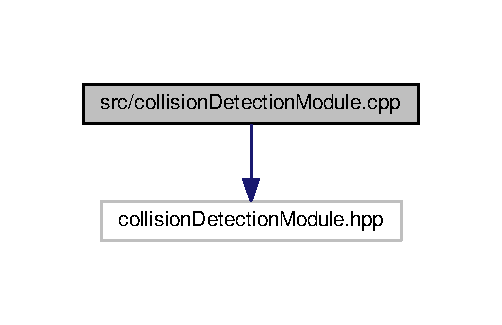
\includegraphics[width=241pt]{collisionDetectionModule_8cpp__incl}
\end{center}
\end{figure}
\subsection*{Functions}
\begin{DoxyCompactItemize}
\item 
segment \hyperlink{collisionDetectionModule_8cpp_ac00660574f32e63039402e0b32829fa0}{get\+Segment} (double x0, double y0, double xf, double yf)
\item 
circle \hyperlink{collisionDetectionModule_8cpp_a75dab4df77767985e71a0f12780c8651}{get\+Circle} (double x, double y, double r)
\item 
void \hyperlink{collisionDetectionModule_8cpp_a8aadc49fbe98b521d9280ce4d0546278}{get\+Plottable\+Segment} (segment L, std\+::vector$<$ double $>$ \&L\+\_\+x\+\_\+data, std\+::vector$<$ double $>$ \&L\+\_\+y\+\_\+data)
\item 
void \hyperlink{collisionDetectionModule_8cpp_ae8155fb328040900e5f0019d27ff64e9}{get\+Plottable\+Circle} (circle c, std\+::vector$<$ double $>$ \&cf\+\_\+x, std\+::vector$<$ double $>$ \&cf\+\_\+y)
\item 
void \hyperlink{collisionDetectionModule_8cpp_a098c5ba24bd0019076010c7208f87c48}{get\+Plottable\+Arc} (arc a, std\+::vector$<$ double $>$ \&arc\+\_\+x\+\_\+data, std\+::vector$<$ double $>$ \&arc\+\_\+y\+\_\+data)
\item 
void \hyperlink{collisionDetectionModule_8cpp_ad524fe2b1726a905d53a8a63f57caa12}{plot\+LL} (segment L1, segment L2)
\item 
void \hyperlink{collisionDetectionModule_8cpp_ad7b5ae148eced1081debc32222e0180e}{plot\+CL} (circle c, segment L)
\item 
void \hyperlink{collisionDetectionModule_8cpp_a895ccddeb129b3fb059660fd45ea00c1}{plot\+AL} (circle c, arc a, segment L, double i\+\_\+x0, double i\+\_\+y0, double i\+\_\+x1, double i\+\_\+y1)
\item 
double \hyperlink{collisionDetectionModule_8cpp_a1686bea7650bb70f997f5c22556f17f5}{get\+Angular\+Coeff} (segment L)
\item 
double \hyperlink{collisionDetectionModule_8cpp_a83e5bb021855b8061a145d056e224da6}{get\+Intercept} (segment L, double m)
\item 
bool \hyperlink{collisionDetectionModule_8cpp_aeb93f834fe94af8aebf6c56cb7e2bd64}{is\+Vertical} (segment L)
\item 
bool \hyperlink{collisionDetectionModule_8cpp_af4abf464c6772933f3fa2ea95f554cbf}{is\+Horizontal} (segment L)
\item 
std\+::tuple$<$ double, double $>$ \hyperlink{collisionDetectionModule_8cpp_a36320729f307de437e3b20710933d441}{get\+Middle\+Pt\+Coords} (segment L)
\item 
double \hyperlink{collisionDetectionModule_8cpp_a1f85cabf7ff9b9b10f885832b0142007}{get\+Segment\+Length} (segment L)
\item 
std\+::tuple$<$ segment, segment $>$ \hyperlink{collisionDetectionModule_8cpp_a1cdc724ae15f2f939a86812d621bed70}{get\+Chords} (arc a)
\item 
circle \hyperlink{collisionDetectionModule_8cpp_a09a74dc2e8976cd645ebf577dc3d2fca}{get\+Cricle\+From\+Arc} (arc a)
\item 
std\+::tuple$<$ bool, double, double $>$ \hyperlink{collisionDetectionModule_8cpp_a32193beac69867b52a5aa634fdccedfc}{inters\+Line\+Line} (segment L1, segment L2)
\item 
std\+::tuple$<$ bool, double, double, double, double, double, double $>$ \hyperlink{collisionDetectionModule_8cpp_aec5cea694b133d876d74b30932ce8177}{inters\+Circle\+Line} (circle c, segment L)
\item 
std\+::tuple$<$ bool, double, double, double, double $>$ \hyperlink{collisionDetectionModule_8cpp_a0455ed7a2a0350cadda022dbf30df873}{inters\+Arc\+Line} (arc a, segment L)
\end{DoxyCompactItemize}


\subsection{Function Documentation}
\index{collision\+Detection\+Module.\+cpp@{collision\+Detection\+Module.\+cpp}!get\+Angular\+Coeff@{get\+Angular\+Coeff}}
\index{get\+Angular\+Coeff@{get\+Angular\+Coeff}!collision\+Detection\+Module.\+cpp@{collision\+Detection\+Module.\+cpp}}
\subsubsection[{\texorpdfstring{get\+Angular\+Coeff(segment L)}{getAngularCoeff(segment L)}}]{\setlength{\rightskip}{0pt plus 5cm}double get\+Angular\+Coeff (
\begin{DoxyParamCaption}
\item[{segment}]{L}
\end{DoxyParamCaption}
)}\hypertarget{collisionDetectionModule_8cpp_a1686bea7650bb70f997f5c22556f17f5}{}\label{collisionDetectionModule_8cpp_a1686bea7650bb70f997f5c22556f17f5}
It returns the angular coefficient of the line passing via the provided segment (i.\+e. m = delta\+\_\+y / delta\+\_\+x). 
\begin{DoxyParams}[1]{Parameters}
\mbox{\tt in}  & {\em L} & Segment. \\
\hline
\end{DoxyParams}
\begin{DoxyReturn}{Returns}
\mbox{[}double\mbox{]} Angular coefficient (i.\+e. m). 
\end{DoxyReturn}
\index{collision\+Detection\+Module.\+cpp@{collision\+Detection\+Module.\+cpp}!get\+Chords@{get\+Chords}}
\index{get\+Chords@{get\+Chords}!collision\+Detection\+Module.\+cpp@{collision\+Detection\+Module.\+cpp}}
\subsubsection[{\texorpdfstring{get\+Chords(arc a)}{getChords(arc a)}}]{\setlength{\rightskip}{0pt plus 5cm}std\+::tuple$<$segment, segment$>$ get\+Chords (
\begin{DoxyParamCaption}
\item[{arc}]{a}
\end{DoxyParamCaption}
)}\hypertarget{collisionDetectionModule_8cpp_a1cdc724ae15f2f939a86812d621bed70}{}\label{collisionDetectionModule_8cpp_a1cdc724ae15f2f939a86812d621bed70}
Retrieves two chords from an arc. None of them is vertical nor horizontal. 
\begin{DoxyParams}[1]{Parameters}
\mbox{\tt in}  & {\em a} & Arc. \\
\hline
\end{DoxyParams}
\begin{DoxyReturn}{Returns}
\mbox{[}std\+::tuple$<$segment, segment$>$\mbox{]} Tuple with 2 segment chords. 
\end{DoxyReturn}
\index{collision\+Detection\+Module.\+cpp@{collision\+Detection\+Module.\+cpp}!get\+Circle@{get\+Circle}}
\index{get\+Circle@{get\+Circle}!collision\+Detection\+Module.\+cpp@{collision\+Detection\+Module.\+cpp}}
\subsubsection[{\texorpdfstring{get\+Circle(double x, double y, double r)}{getCircle(double x, double y, double r)}}]{\setlength{\rightskip}{0pt plus 5cm}circle get\+Circle (
\begin{DoxyParamCaption}
\item[{double}]{x, }
\item[{double}]{y, }
\item[{double}]{r}
\end{DoxyParamCaption}
)}\hypertarget{collisionDetectionModule_8cpp_a75dab4df77767985e71a0f12780c8651}{}\label{collisionDetectionModule_8cpp_a75dab4df77767985e71a0f12780c8651}
Create a structure representing a circle. 
\begin{DoxyParams}[1]{Parameters}
\mbox{\tt in}  & {\em x} & Center x-\/coord. \\
\hline
\mbox{\tt in}  & {\em y} & Center y-\/coord. \\
\hline
\mbox{\tt in}  & {\em r} & Radius of the circle. \\
\hline
\end{DoxyParams}
\begin{DoxyReturn}{Returns}
\mbox{[}circle\mbox{]} c Circle type. 
\end{DoxyReturn}
\index{collision\+Detection\+Module.\+cpp@{collision\+Detection\+Module.\+cpp}!get\+Cricle\+From\+Arc@{get\+Cricle\+From\+Arc}}
\index{get\+Cricle\+From\+Arc@{get\+Cricle\+From\+Arc}!collision\+Detection\+Module.\+cpp@{collision\+Detection\+Module.\+cpp}}
\subsubsection[{\texorpdfstring{get\+Cricle\+From\+Arc(arc a)}{getCricleFromArc(arc a)}}]{\setlength{\rightskip}{0pt plus 5cm}circle get\+Cricle\+From\+Arc (
\begin{DoxyParamCaption}
\item[{arc}]{a}
\end{DoxyParamCaption}
)}\hypertarget{collisionDetectionModule_8cpp_a09a74dc2e8976cd645ebf577dc3d2fca}{}\label{collisionDetectionModule_8cpp_a09a74dc2e8976cd645ebf577dc3d2fca}
Given a dubins arc it returns the corresponding circle. It finds two chords within the arc. Then i looks for chords bisectors. In the end, from the bisectors intersection, it finds the center. 
\begin{DoxyParams}[1]{Parameters}
\mbox{\tt in}  & {\em a} & Arc. \\
\hline
\end{DoxyParams}
\begin{DoxyReturn}{Returns}
\mbox{[}circle\mbox{]} Circle derived from the provided arc. 
\end{DoxyReturn}
\index{collision\+Detection\+Module.\+cpp@{collision\+Detection\+Module.\+cpp}!get\+Intercept@{get\+Intercept}}
\index{get\+Intercept@{get\+Intercept}!collision\+Detection\+Module.\+cpp@{collision\+Detection\+Module.\+cpp}}
\subsubsection[{\texorpdfstring{get\+Intercept(segment L, double m)}{getIntercept(segment L, double m)}}]{\setlength{\rightskip}{0pt plus 5cm}double get\+Intercept (
\begin{DoxyParamCaption}
\item[{segment}]{L, }
\item[{double}]{m}
\end{DoxyParamCaption}
)}\hypertarget{collisionDetectionModule_8cpp_a83e5bb021855b8061a145d056e224da6}{}\label{collisionDetectionModule_8cpp_a83e5bb021855b8061a145d056e224da6}
It returns the intercept of the line passing via the provided segment with a given angular coefficient. 
\begin{DoxyParams}[1]{Parameters}
\mbox{\tt in}  & {\em L} & Segment. \\
\hline
\mbox{\tt in}  & {\em m} & Angular coefficient of the line passing via L. \\
\hline
\end{DoxyParams}
\begin{DoxyReturn}{Returns}
\mbox{[}double\mbox{]} Intercept (i.\+e. q). 
\end{DoxyReturn}
\index{collision\+Detection\+Module.\+cpp@{collision\+Detection\+Module.\+cpp}!get\+Middle\+Pt\+Coords@{get\+Middle\+Pt\+Coords}}
\index{get\+Middle\+Pt\+Coords@{get\+Middle\+Pt\+Coords}!collision\+Detection\+Module.\+cpp@{collision\+Detection\+Module.\+cpp}}
\subsubsection[{\texorpdfstring{get\+Middle\+Pt\+Coords(segment L)}{getMiddlePtCoords(segment L)}}]{\setlength{\rightskip}{0pt plus 5cm}std\+::tuple$<$double, double$>$ get\+Middle\+Pt\+Coords (
\begin{DoxyParamCaption}
\item[{segment}]{L}
\end{DoxyParamCaption}
)}\hypertarget{collisionDetectionModule_8cpp_a36320729f307de437e3b20710933d441}{}\label{collisionDetectionModule_8cpp_a36320729f307de437e3b20710933d441}
Given a segment it returns the middle point coordinates. 
\begin{DoxyParams}[1]{Parameters}
\mbox{\tt in}  & {\em L} & Segment. \\
\hline
\end{DoxyParams}
\begin{DoxyReturn}{Returns}
\mbox{[}std\+::tuple$<$double, double$>$\mbox{]} Tuple with x-\/coord and y-\/coord. 
\end{DoxyReturn}
\index{collision\+Detection\+Module.\+cpp@{collision\+Detection\+Module.\+cpp}!get\+Plottable\+Arc@{get\+Plottable\+Arc}}
\index{get\+Plottable\+Arc@{get\+Plottable\+Arc}!collision\+Detection\+Module.\+cpp@{collision\+Detection\+Module.\+cpp}}
\subsubsection[{\texorpdfstring{get\+Plottable\+Arc(arc a, std\+::vector$<$ double $>$ \&arc\+\_\+x\+\_\+data, std\+::vector$<$ double $>$ \&arc\+\_\+y\+\_\+data)}{getPlottableArc(arc a, std::vector< double > &arc_x_data, std::vector< double > &arc_y_data)}}]{\setlength{\rightskip}{0pt plus 5cm}void get\+Plottable\+Arc (
\begin{DoxyParamCaption}
\item[{arc}]{a, }
\item[{std\+::vector$<$ double $>$ \&}]{arc\+\_\+x\+\_\+data, }
\item[{std\+::vector$<$ double $>$ \&}]{arc\+\_\+y\+\_\+data}
\end{DoxyParamCaption}
)}\hypertarget{collisionDetectionModule_8cpp_a098c5ba24bd0019076010c7208f87c48}{}\label{collisionDetectionModule_8cpp_a098c5ba24bd0019076010c7208f87c48}
Retrieves the two vectors\+: the former is filled with arc x-\/coords and the latter with arc y-\/coords. 
\begin{DoxyParams}[1]{Parameters}
\mbox{\tt in}  & {\em a} & Arc. \\
\hline
\mbox{\tt out}  & {\em L\+\_\+x\+\_\+data} & Vector of x-\/coords. \\
\hline
\mbox{\tt out}  & {\em L\+\_\+y\+\_\+data} & Vector of y-\/coords. \\
\hline
\end{DoxyParams}
\index{collision\+Detection\+Module.\+cpp@{collision\+Detection\+Module.\+cpp}!get\+Plottable\+Circle@{get\+Plottable\+Circle}}
\index{get\+Plottable\+Circle@{get\+Plottable\+Circle}!collision\+Detection\+Module.\+cpp@{collision\+Detection\+Module.\+cpp}}
\subsubsection[{\texorpdfstring{get\+Plottable\+Circle(circle c, std\+::vector$<$ double $>$ \&cf\+\_\+x, std\+::vector$<$ double $>$ \&cf\+\_\+y)}{getPlottableCircle(circle c, std::vector< double > &cf_x, std::vector< double > &cf_y)}}]{\setlength{\rightskip}{0pt plus 5cm}void get\+Plottable\+Circle (
\begin{DoxyParamCaption}
\item[{circle}]{c, }
\item[{std\+::vector$<$ double $>$ \&}]{cf\+\_\+x, }
\item[{std\+::vector$<$ double $>$ \&}]{cf\+\_\+y}
\end{DoxyParamCaption}
)}\hypertarget{collisionDetectionModule_8cpp_ae8155fb328040900e5f0019d27ff64e9}{}\label{collisionDetectionModule_8cpp_ae8155fb328040900e5f0019d27ff64e9}
Retrieves the two vectors\+: the former is filled with circle x-\/coords and the latter with circle y-\/coords. 
\begin{DoxyParams}[1]{Parameters}
\mbox{\tt in}  & {\em c} & Circle. \\
\hline
\mbox{\tt out}  & {\em L\+\_\+x\+\_\+data} & Vector of x-\/coords. \\
\hline
\mbox{\tt out}  & {\em L\+\_\+y\+\_\+data} & Vector of y-\/coords. \\
\hline
\end{DoxyParams}
\index{collision\+Detection\+Module.\+cpp@{collision\+Detection\+Module.\+cpp}!get\+Plottable\+Segment@{get\+Plottable\+Segment}}
\index{get\+Plottable\+Segment@{get\+Plottable\+Segment}!collision\+Detection\+Module.\+cpp@{collision\+Detection\+Module.\+cpp}}
\subsubsection[{\texorpdfstring{get\+Plottable\+Segment(segment L, std\+::vector$<$ double $>$ \&\+L\+\_\+x\+\_\+data, std\+::vector$<$ double $>$ \&\+L\+\_\+y\+\_\+data)}{getPlottableSegment(segment L, std::vector< double > &L_x_data, std::vector< double > &L_y_data)}}]{\setlength{\rightskip}{0pt plus 5cm}void get\+Plottable\+Segment (
\begin{DoxyParamCaption}
\item[{segment}]{L, }
\item[{std\+::vector$<$ double $>$ \&}]{L\+\_\+x\+\_\+data, }
\item[{std\+::vector$<$ double $>$ \&}]{L\+\_\+y\+\_\+data}
\end{DoxyParamCaption}
)}\hypertarget{collisionDetectionModule_8cpp_a8aadc49fbe98b521d9280ce4d0546278}{}\label{collisionDetectionModule_8cpp_a8aadc49fbe98b521d9280ce4d0546278}
Retrieves the two vectors\+: the former is filled with segment x-\/coords and the latter with segment y-\/coords. 
\begin{DoxyParams}[1]{Parameters}
\mbox{\tt in}  & {\em L} & Segment. \\
\hline
\mbox{\tt out}  & {\em L\+\_\+x\+\_\+data} & Vector of x-\/coords. \\
\hline
\mbox{\tt out}  & {\em L\+\_\+y\+\_\+data} & Vector of y-\/coords. \\
\hline
\end{DoxyParams}
\index{collision\+Detection\+Module.\+cpp@{collision\+Detection\+Module.\+cpp}!get\+Segment@{get\+Segment}}
\index{get\+Segment@{get\+Segment}!collision\+Detection\+Module.\+cpp@{collision\+Detection\+Module.\+cpp}}
\subsubsection[{\texorpdfstring{get\+Segment(double x0, double y0, double xf, double yf)}{getSegment(double x0, double y0, double xf, double yf)}}]{\setlength{\rightskip}{0pt plus 5cm}segment get\+Segment (
\begin{DoxyParamCaption}
\item[{double}]{x0, }
\item[{double}]{y0, }
\item[{double}]{xf, }
\item[{double}]{yf}
\end{DoxyParamCaption}
)}\hypertarget{collisionDetectionModule_8cpp_ac00660574f32e63039402e0b32829fa0}{}\label{collisionDetectionModule_8cpp_ac00660574f32e63039402e0b32829fa0}
Create a structure representing a segment. 
\begin{DoxyParams}[1]{Parameters}
\mbox{\tt in}  & {\em x0} & Initial x-\/coord. \\
\hline
\mbox{\tt in}  & {\em y0} & Initial y-\/coord. \\
\hline
\mbox{\tt in}  & {\em xf} & Final x-\/coord. \\
\hline
\mbox{\tt in}  & {\em yf} & Final y-\/coord. \\
\hline
\end{DoxyParams}
\begin{DoxyReturn}{Returns}
\mbox{[}segment\mbox{]} L Segment type. 
\end{DoxyReturn}
\index{collision\+Detection\+Module.\+cpp@{collision\+Detection\+Module.\+cpp}!get\+Segment\+Length@{get\+Segment\+Length}}
\index{get\+Segment\+Length@{get\+Segment\+Length}!collision\+Detection\+Module.\+cpp@{collision\+Detection\+Module.\+cpp}}
\subsubsection[{\texorpdfstring{get\+Segment\+Length(segment L)}{getSegmentLength(segment L)}}]{\setlength{\rightskip}{0pt plus 5cm}double get\+Segment\+Length (
\begin{DoxyParamCaption}
\item[{segment}]{L}
\end{DoxyParamCaption}
)}\hypertarget{collisionDetectionModule_8cpp_a1f85cabf7ff9b9b10f885832b0142007}{}\label{collisionDetectionModule_8cpp_a1f85cabf7ff9b9b10f885832b0142007}
It returns the the length of a given segment. 
\begin{DoxyParams}[1]{Parameters}
\mbox{\tt in}  & {\em L} & Segment. \\
\hline
\end{DoxyParams}
\begin{DoxyReturn}{Returns}
\mbox{[}double\mbox{]} Tuple with x-\/coord and y-\/coord. 
\end{DoxyReturn}
\index{collision\+Detection\+Module.\+cpp@{collision\+Detection\+Module.\+cpp}!inters\+Arc\+Line@{inters\+Arc\+Line}}
\index{inters\+Arc\+Line@{inters\+Arc\+Line}!collision\+Detection\+Module.\+cpp@{collision\+Detection\+Module.\+cpp}}
\subsubsection[{\texorpdfstring{inters\+Arc\+Line(arc a, segment L)}{intersArcLine(arc a, segment L)}}]{\setlength{\rightskip}{0pt plus 5cm}std\+::tuple$<$bool, double, double, double, double$>$ inters\+Arc\+Line (
\begin{DoxyParamCaption}
\item[{arc}]{a, }
\item[{segment}]{L}
\end{DoxyParamCaption}
)}\hypertarget{collisionDetectionModule_8cpp_a0455ed7a2a0350cadda022dbf30df873}{}\label{collisionDetectionModule_8cpp_a0455ed7a2a0350cadda022dbf30df873}
Determine if there is an intersection between an arc of a circle and a segment. If there is an intersection it returns also the coords. 
\begin{DoxyParams}[1]{Parameters}
\mbox{\tt in}  & {\em a} & Arc. \\
\hline
\mbox{\tt in}  & {\em L} & Segment. \\
\hline
\end{DoxyParams}
\begin{DoxyReturn}{Returns}
\mbox{[}std\+::tuple$<$bool, double, double, double, double$>$\mbox{]} Tuple with bool true if intersection exists, 1st intersection (x-\/coord, y-\/coord), 2nd intersection (x-\/coord, y-\/coord). 
\end{DoxyReturn}
\index{collision\+Detection\+Module.\+cpp@{collision\+Detection\+Module.\+cpp}!inters\+Circle\+Line@{inters\+Circle\+Line}}
\index{inters\+Circle\+Line@{inters\+Circle\+Line}!collision\+Detection\+Module.\+cpp@{collision\+Detection\+Module.\+cpp}}
\subsubsection[{\texorpdfstring{inters\+Circle\+Line(circle c, segment L)}{intersCircleLine(circle c, segment L)}}]{\setlength{\rightskip}{0pt plus 5cm}std\+::tuple$<$bool, double, double, double, double, double, double$>$ inters\+Circle\+Line (
\begin{DoxyParamCaption}
\item[{circle}]{c, }
\item[{segment}]{L}
\end{DoxyParamCaption}
)}\hypertarget{collisionDetectionModule_8cpp_aec5cea694b133d876d74b30932ce8177}{}\label{collisionDetectionModule_8cpp_aec5cea694b133d876d74b30932ce8177}
Determine if there is an intersection between a circle and a segment. If there is an intersection it returns also the coords. 
\begin{DoxyParams}[1]{Parameters}
\mbox{\tt in}  & {\em c} & Circle. \\
\hline
\mbox{\tt in}  & {\em L} & Segment. \\
\hline
\end{DoxyParams}
\begin{DoxyReturn}{Returns}
\mbox{[}std\+::tuple$<$bool, double, double, double, double, double, double$>$\mbox{]} Tuple with bool true if intersection exists, 1st intersection (x-\/coord, y-\/coord), 1st intersection angle w.\+r.\+t. center, 2nd intersection (x-\/coord, y-\/coord), 2nd intersection angle w.\+r.\+t. center. 
\end{DoxyReturn}
\index{collision\+Detection\+Module.\+cpp@{collision\+Detection\+Module.\+cpp}!inters\+Line\+Line@{inters\+Line\+Line}}
\index{inters\+Line\+Line@{inters\+Line\+Line}!collision\+Detection\+Module.\+cpp@{collision\+Detection\+Module.\+cpp}}
\subsubsection[{\texorpdfstring{inters\+Line\+Line(segment L1, segment L2)}{intersLineLine(segment L1, segment L2)}}]{\setlength{\rightskip}{0pt plus 5cm}std\+::tuple$<$bool, double, double$>$ inters\+Line\+Line (
\begin{DoxyParamCaption}
\item[{segment}]{L1, }
\item[{segment}]{L2}
\end{DoxyParamCaption}
)}\hypertarget{collisionDetectionModule_8cpp_a32193beac69867b52a5aa634fdccedfc}{}\label{collisionDetectionModule_8cpp_a32193beac69867b52a5aa634fdccedfc}
Determine if there is an intersection between two segments. If there is an intersection it returns also the coords. 
\begin{DoxyParams}[1]{Parameters}
\mbox{\tt in}  & {\em L1} & First segment. \\
\hline
\mbox{\tt in}  & {\em L2} & Second segment. \\
\hline
\mbox{\tt out}  & {\em $<$flag\+\_\+i,x,y$>$} & Tuple with bool true if intersection exists, intersection (x-\/coord, y-\/coord). \\
\hline
\end{DoxyParams}
\index{collision\+Detection\+Module.\+cpp@{collision\+Detection\+Module.\+cpp}!is\+Horizontal@{is\+Horizontal}}
\index{is\+Horizontal@{is\+Horizontal}!collision\+Detection\+Module.\+cpp@{collision\+Detection\+Module.\+cpp}}
\subsubsection[{\texorpdfstring{is\+Horizontal(segment L)}{isHorizontal(segment L)}}]{\setlength{\rightskip}{0pt plus 5cm}bool is\+Horizontal (
\begin{DoxyParamCaption}
\item[{segment}]{L}
\end{DoxyParamCaption}
)}\hypertarget{collisionDetectionModule_8cpp_af4abf464c6772933f3fa2ea95f554cbf}{}\label{collisionDetectionModule_8cpp_af4abf464c6772933f3fa2ea95f554cbf}
Given a segment it returns true if it is horizontal (i.\+e. angular coeff = 0). 
\begin{DoxyParams}[1]{Parameters}
\mbox{\tt in}  & {\em L} & Segment. \\
\hline
\end{DoxyParams}
\begin{DoxyReturn}{Returns}
\mbox{[}bool\mbox{]} True if horizontal, false otherwise. 
\end{DoxyReturn}
\index{collision\+Detection\+Module.\+cpp@{collision\+Detection\+Module.\+cpp}!is\+Vertical@{is\+Vertical}}
\index{is\+Vertical@{is\+Vertical}!collision\+Detection\+Module.\+cpp@{collision\+Detection\+Module.\+cpp}}
\subsubsection[{\texorpdfstring{is\+Vertical(segment L)}{isVertical(segment L)}}]{\setlength{\rightskip}{0pt plus 5cm}bool is\+Vertical (
\begin{DoxyParamCaption}
\item[{segment}]{L}
\end{DoxyParamCaption}
)}\hypertarget{collisionDetectionModule_8cpp_aeb93f834fe94af8aebf6c56cb7e2bd64}{}\label{collisionDetectionModule_8cpp_aeb93f834fe94af8aebf6c56cb7e2bd64}
Given a segment it returns true if it is verticla (i.\+e. angular coeff = I\+NF). 
\begin{DoxyParams}[1]{Parameters}
\mbox{\tt in}  & {\em L} & Segment. \\
\hline
\end{DoxyParams}
\begin{DoxyReturn}{Returns}
\mbox{[}bool\mbox{]} True if vertical, false otherwise. 
\end{DoxyReturn}
\index{collision\+Detection\+Module.\+cpp@{collision\+Detection\+Module.\+cpp}!plot\+AL@{plot\+AL}}
\index{plot\+AL@{plot\+AL}!collision\+Detection\+Module.\+cpp@{collision\+Detection\+Module.\+cpp}}
\subsubsection[{\texorpdfstring{plot\+A\+L(circle c, arc a, segment L, double i\+\_\+x0, double i\+\_\+y0, double i\+\_\+x1, double i\+\_\+y1)}{plotAL(circle c, arc a, segment L, double i_x0, double i_y0, double i_x1, double i_y1)}}]{\setlength{\rightskip}{0pt plus 5cm}void plot\+AL (
\begin{DoxyParamCaption}
\item[{circle}]{c, }
\item[{arc}]{a, }
\item[{segment}]{L, }
\item[{double}]{i\+\_\+x0, }
\item[{double}]{i\+\_\+y0, }
\item[{double}]{i\+\_\+x1, }
\item[{double}]{i\+\_\+y1}
\end{DoxyParamCaption}
)}\hypertarget{collisionDetectionModule_8cpp_a895ccddeb129b3fb059660fd45ea00c1}{}\label{collisionDetectionModule_8cpp_a895ccddeb129b3fb059660fd45ea00c1}
It plots an arc and a segment and save it as Arc\+\_\+segment\+\_\+intersection.\+png in /home/user\+\_\+name/workspace/project/src/testing\+\_\+imgs . 
\begin{DoxyParams}[1]{Parameters}
\mbox{\tt in}  & {\em c} & Circle. \\
\hline
\mbox{\tt in}  & {\em a} & Arc. \\
\hline
\mbox{\tt in}  & {\em L} & Segment. \\
\hline
\mbox{\tt in}  & {\em i\+\_\+x0} & First intersection point x-\/coord. \\
\hline
\mbox{\tt in}  & {\em i\+\_\+y0} & First intersection point y-\/coord. \\
\hline
\mbox{\tt in}  & {\em i\+\_\+x1} & Second intersection point x-\/coord. \\
\hline
\mbox{\tt in}  & {\em i\+\_\+y1} & Second intersection point y-\/coord. \\
\hline
\end{DoxyParams}
\index{collision\+Detection\+Module.\+cpp@{collision\+Detection\+Module.\+cpp}!plot\+CL@{plot\+CL}}
\index{plot\+CL@{plot\+CL}!collision\+Detection\+Module.\+cpp@{collision\+Detection\+Module.\+cpp}}
\subsubsection[{\texorpdfstring{plot\+C\+L(circle c, segment L)}{plotCL(circle c, segment L)}}]{\setlength{\rightskip}{0pt plus 5cm}void plot\+CL (
\begin{DoxyParamCaption}
\item[{circle}]{c, }
\item[{segment}]{L}
\end{DoxyParamCaption}
)}\hypertarget{collisionDetectionModule_8cpp_ad7b5ae148eced1081debc32222e0180e}{}\label{collisionDetectionModule_8cpp_ad7b5ae148eced1081debc32222e0180e}
It plots a circle and a segment and save it as Circle\+\_\+segment\+\_\+intersection.\+png in /home/user\+\_\+name/workspace/project/src/testing\+\_\+imgs . 
\begin{DoxyParams}[1]{Parameters}
\mbox{\tt in}  & {\em c} & Circle. \\
\hline
\mbox{\tt in}  & {\em L} & Segment. \\
\hline
\end{DoxyParams}
\index{collision\+Detection\+Module.\+cpp@{collision\+Detection\+Module.\+cpp}!plot\+LL@{plot\+LL}}
\index{plot\+LL@{plot\+LL}!collision\+Detection\+Module.\+cpp@{collision\+Detection\+Module.\+cpp}}
\subsubsection[{\texorpdfstring{plot\+L\+L(segment L1, segment L2)}{plotLL(segment L1, segment L2)}}]{\setlength{\rightskip}{0pt plus 5cm}void plot\+LL (
\begin{DoxyParamCaption}
\item[{segment}]{L1, }
\item[{segment}]{L2}
\end{DoxyParamCaption}
)}\hypertarget{collisionDetectionModule_8cpp_ad524fe2b1726a905d53a8a63f57caa12}{}\label{collisionDetectionModule_8cpp_ad524fe2b1726a905d53a8a63f57caa12}
It plots two segments and save it as Segmentss\+\_\+intersection.\+png. in /home/user\+\_\+name/workspace/project/src/testing\+\_\+imgs . 
\begin{DoxyParams}[1]{Parameters}
\mbox{\tt in}  & {\em L1} & Arc. \\
\hline
\mbox{\tt in}  & {\em L2} & Vector of x-\/coords. \\
\hline
\end{DoxyParams}

\hypertarget{dubins_8cpp}{}\section{src/dubins.cpp File Reference}
\label{dubins_8cpp}\index{src/dubins.\+cpp@{src/dubins.\+cpp}}
{\ttfamily \#include \char`\"{}dubins.\+hpp\char`\"{}}\\*
Include dependency graph for dubins.\+cpp\+:\nopagebreak
\begin{figure}[H]
\begin{center}
\leavevmode
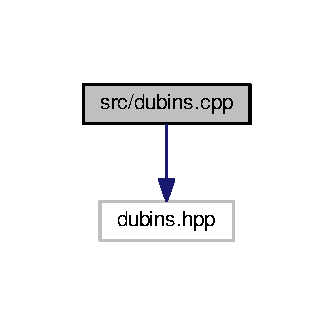
\includegraphics[width=160pt]{dubins_8cpp__incl}
\end{center}
\end{figure}
\subsection*{Functions}
\begin{DoxyCompactItemize}
\item 
double \hyperlink{dubins_8cpp_a2678c9ac5e8585534a9c5a2385169324}{sinc} (double t)
\item 
double \hyperlink{dubins_8cpp_a2c708c33a19d61b2cdb44cc19fc6b0d9}{mod2pi} (double ang)
\item 
double \hyperlink{dubins_8cpp_a994d30c469683c4818f820919609fc84}{range\+Symm} (double ang)
\item 
std\+::tuple$<$ double, double, double $>$ \hyperlink{dubins_8cpp_a7553fe315735742bcf80b97dd915df85}{circline} (double s, double x0, double y0, double th0, double k)
\item 
bool \hyperlink{dubins_8cpp_ae399651dd05d7ddca1755495526568b2}{check} (double s1, double k0, double s2, double k1, double s3, double k2, double th0, double thf)
\item 
arc \hyperlink{dubins_8cpp_a6427aadaeacca9d1b07f6244aa3180b9}{get\+Dubins\+Arc} (double x0, double y0, double th0, double k, double L)
\item 
curve \hyperlink{dubins_8cpp_a1c265c884e9666b566b125499516c297}{get\+Dubins\+Curve} (double x0, double y0, double th0, double s1, double s2, double s3, double k0, double k1, double k2)
\item 
std\+::tuple$<$ double, double, double, double $>$ \hyperlink{dubins_8cpp_a494897b7ad240d3f473773ad5e75e3b2}{scale\+Orig2\+Std} (double x0, double y0, double th0, double xf, double yf, double thf, double Kmax)
\item 
std\+::tuple$<$ double, double, double $>$ \hyperlink{dubins_8cpp_aea31016ab837046cbd5a783dc363e727}{scale\+Std2\+Orig} (double lambda, double sc\+\_\+s1, double sc\+\_\+s2, double sc\+\_\+s3)
\item 
std\+::tuple$<$ bool, double, double, double $>$ \hyperlink{dubins_8cpp_ac4b7ba8f16b5e9bcac53b64de87d3b58}{L\+SL} (double sc\+\_\+th0, double sc\+\_\+thf, double sc\+\_\+\+Kmax)
\item 
std\+::tuple$<$ bool, double, double, double $>$ \hyperlink{dubins_8cpp_a0b8a278bd4f3c3dcdaa39e1303802c75}{R\+SR} (double sc\+\_\+th0, double sc\+\_\+thf, double sc\+\_\+\+Kmax)
\item 
std\+::tuple$<$ bool, double, double, double $>$ \hyperlink{dubins_8cpp_aefe1b61b500009a2142e4247d831b1e5}{L\+SR} (double sc\+\_\+th0, double sc\+\_\+thf, double sc\+\_\+\+Kmax)
\item 
std\+::tuple$<$ bool, double, double, double $>$ \hyperlink{dubins_8cpp_ad6625b8d3efc7ec0beb9e2fb5b040566}{R\+SL} (double sc\+\_\+th0, double sc\+\_\+thf, double sc\+\_\+\+Kmax)
\item 
std\+::tuple$<$ bool, double, double, double $>$ \hyperlink{dubins_8cpp_a56275bfea544ace5891df19f92b97551}{R\+LR} (double sc\+\_\+th0, double sc\+\_\+thf, double sc\+\_\+\+Kmax)
\item 
std\+::tuple$<$ bool, double, double, double $>$ \hyperlink{dubins_8cpp_a0a1120a592fbc3c932d8530d56aa794a}{L\+RL} (double sc\+\_\+th0, double sc\+\_\+thf, double sc\+\_\+\+Kmax)
\item 
std\+::pair$<$ int, curve $>$ \hyperlink{dubins_8cpp_a7caccbbd59a4d324e59e9e19e00b38af}{dubins\+\_\+shortest\+\_\+path} (double x0, double y0, double th0, double xf, double yf, double thf, double Kmax)
\item 
std\+::tuple$<$ std\+::vector$<$ double $>$, std\+::vector$<$ double $>$ $>$ \hyperlink{dubins_8cpp_afaea347e8dd6b21dd770f8b67b85763f}{get\+Plottable\+Arc} (arc a)
\item 
void \hyperlink{dubins_8cpp_a75e4caf509feca2e1dfa379cecea9744}{plot\+Dubins} (curve c)
\item 
void \hyperlink{dubins_8cpp_a283f1c1d10ae03dbfc3a03ceaabf08e8}{plot\+Multi\+Dubins} (std\+::vector$<$ std\+::pair$<$ int, curve $>$$>$ all\+\_\+best\+\_\+curves)
\item 
void \hyperlink{dubins_8cpp_a7e9cda9b85a07e92a80003c84c5cccb0}{get\+Angles} (double k\+\_\+thj, std\+::vector$<$ double $>$ \&all\+\_\+thj)
\item 
void \hyperlink{dubins_8cpp_afc4d12795d09ee2032a41fe8b255b61c}{get\+Angles\+RS} (double m, double k\+\_\+thj, double prev\+\_\+thj, std\+::vector$<$ double $>$ \&all\+\_\+thj\+\_\+rs)
\item 
void \hyperlink{dubins_8cpp_a151abe27330eb4577f8b09bc7f7be6f7}{min\+Dj} (double x\+\_\+prev, double y\+\_\+prev, std\+::vector$<$ double $>$ \&all\+\_\+thj, double x\+\_\+last, double y\+\_\+last, double th\+\_\+last, double Kmax, std\+::tuple$<$ double, int, curve $>$ \&min\+Dj\+\_\+result)
\item 
void \hyperlink{dubins_8cpp_adbcb267c908e72a53312ff0fd21e56b2}{refinement\+Steps} (double m, double k\+\_\+thj, double x\+\_\+prev, double y\+\_\+prev, double x\+\_\+last, double y\+\_\+last, double th\+\_\+last, double Kmax, std\+::tuple$<$ double, int, curve $>$ \&min\+Dj\+\_\+result)
\end{DoxyCompactItemize}


\subsection{Function Documentation}
\index{dubins.\+cpp@{dubins.\+cpp}!check@{check}}
\index{check@{check}!dubins.\+cpp@{dubins.\+cpp}}
\subsubsection[{\texorpdfstring{check(double s1, double k0, double s2, double k1, double s3, double k2, double th0, double thf)}{check(double s1, double k0, double s2, double k1, double s3, double k2, double th0, double thf)}}]{\setlength{\rightskip}{0pt plus 5cm}bool check (
\begin{DoxyParamCaption}
\item[{double}]{s1, }
\item[{double}]{k0, }
\item[{double}]{s2, }
\item[{double}]{k1, }
\item[{double}]{s3, }
\item[{double}]{k2, }
\item[{double}]{th0, }
\item[{double}]{thf}
\end{DoxyParamCaption}
)}\hypertarget{dubins_8cpp_ae399651dd05d7ddca1755495526568b2}{}\label{dubins_8cpp_ae399651dd05d7ddca1755495526568b2}
Check validity of a solution by evaluating explicitly the 3 equations defining a Dubins problem (in standard form). 
\begin{DoxyParams}[1]{Parameters}
\mbox{\tt in}  & {\em s1} & First arc length. \\
\hline
\mbox{\tt in}  & {\em k0} & First arc max curvature. \\
\hline
\mbox{\tt in}  & {\em s2} & Second arc length. \\
\hline
\mbox{\tt in}  & {\em k1} & Second arc max curvature. \\
\hline
\mbox{\tt in}  & {\em s3} & Third arc length. \\
\hline
\mbox{\tt in}  & {\em k2} & Third arc max curvature. \\
\hline
\mbox{\tt in}  & {\em th0} & Initial angle direction. \\
\hline
\mbox{\tt in}  & {\em thf} & Final angle direction. \\
\hline
\mbox{\tt out}  & {\em check\+\_\+val} & True if the 3 equations are satisfied. \\
\hline
\end{DoxyParams}
\index{dubins.\+cpp@{dubins.\+cpp}!circline@{circline}}
\index{circline@{circline}!dubins.\+cpp@{dubins.\+cpp}}
\subsubsection[{\texorpdfstring{circline(double s, double x0, double y0, double th0, double k)}{circline(double s, double x0, double y0, double th0, double k)}}]{\setlength{\rightskip}{0pt plus 5cm}std\+::tuple$<$double, double, double$>$ circline (
\begin{DoxyParamCaption}
\item[{double}]{s, }
\item[{double}]{x0, }
\item[{double}]{y0, }
\item[{double}]{th0, }
\item[{double}]{k}
\end{DoxyParamCaption}
)}\hypertarget{dubins_8cpp_a7553fe315735742bcf80b97dd915df85}{}\label{dubins_8cpp_a7553fe315735742bcf80b97dd915df85}
Evaluate an arc (circular or straight) composing a Dubins curve, at a given arc-\/length s. 
\begin{DoxyParams}[1]{Parameters}
\mbox{\tt in}  & {\em s} & Arc length. \\
\hline
\mbox{\tt in}  & {\em x0} & Initial x-\/coord. \\
\hline
\mbox{\tt in}  & {\em y0} & Initial y-\/coord. \\
\hline
\mbox{\tt in}  & {\em th0} & Initial angle direction. \\
\hline
\mbox{\tt in}  & {\em k} & Max curvature. \\
\hline
\mbox{\tt out}  & {\em $<$x,y,th$>$} & Final position and direction. \\
\hline
\end{DoxyParams}
\index{dubins.\+cpp@{dubins.\+cpp}!dubins\+\_\+shortest\+\_\+path@{dubins\+\_\+shortest\+\_\+path}}
\index{dubins\+\_\+shortest\+\_\+path@{dubins\+\_\+shortest\+\_\+path}!dubins.\+cpp@{dubins.\+cpp}}
\subsubsection[{\texorpdfstring{dubins\+\_\+shortest\+\_\+path(double x0, double y0, double th0, double xf, double yf, double thf, double Kmax)}{dubins_shortest_path(double x0, double y0, double th0, double xf, double yf, double thf, double Kmax)}}]{\setlength{\rightskip}{0pt plus 5cm}std\+::pair$<$int, curve$>$ dubins\+\_\+shortest\+\_\+path (
\begin{DoxyParamCaption}
\item[{double}]{x0, }
\item[{double}]{y0, }
\item[{double}]{th0, }
\item[{double}]{xf, }
\item[{double}]{yf, }
\item[{double}]{thf, }
\item[{double}]{Kmax}
\end{DoxyParamCaption}
)}\hypertarget{dubins_8cpp_a7caccbbd59a4d324e59e9e19e00b38af}{}\label{dubins_8cpp_a7caccbbd59a4d324e59e9e19e00b38af}
Solve the Dubins problem for the given input parameters. Return the type and the parameters of the optimal curve. 
\begin{DoxyParams}[1]{Parameters}
\mbox{\tt in}  & {\em x0} & Initial x-\/coord. \\
\hline
\mbox{\tt in}  & {\em y0} & Initial y-\/coord. \\
\hline
\mbox{\tt in}  & {\em th0} & Initial angle direction. \\
\hline
\mbox{\tt in}  & {\em xf} & Final x-\/coord. \\
\hline
\mbox{\tt in}  & {\em yf} & Final y-\/coord. \\
\hline
\mbox{\tt in}  & {\em thf} & Final angle direction. \\
\hline
\mbox{\tt in}  & {\em Kmax} & Maximum curvature. \\
\hline
\mbox{\tt out}  & {\em $<$pidx,c$>$} & Pair with best primitive idx and best curve. \\
\hline
\end{DoxyParams}
\index{dubins.\+cpp@{dubins.\+cpp}!get\+Angles@{get\+Angles}}
\index{get\+Angles@{get\+Angles}!dubins.\+cpp@{dubins.\+cpp}}
\subsubsection[{\texorpdfstring{get\+Angles(double k\+\_\+thj, std\+::vector$<$ double $>$ \&all\+\_\+thj)}{getAngles(double k_thj, std::vector< double > &all_thj)}}]{\setlength{\rightskip}{0pt plus 5cm}void get\+Angles (
\begin{DoxyParamCaption}
\item[{double}]{k\+\_\+thj, }
\item[{std\+::vector$<$ double $>$ \&}]{all\+\_\+thj}
\end{DoxyParamCaption}
)}\hypertarget{dubins_8cpp_a7e9cda9b85a07e92a80003c84c5cccb0}{}\label{dubins_8cpp_a7e9cda9b85a07e92a80003c84c5cccb0}
Retrieves the k\+\_\+thj possible theta\+\_\+j angles that have to be tested in order to find the shortest Dubins path. All theta\+\_\+j are normalized in range \mbox{[}0, 2$\ast$\+M\+\_\+\+PI). 
\begin{DoxyParams}[1]{Parameters}
\mbox{\tt in}  & {\em k\+\_\+thj} & Granularity of angle discretization\+: number of theta\+\_\+j. \\
\hline
\mbox{\tt out}  & {\em all\+\_\+thj} & Vector with all angles in the discretized interval. \\
\hline
\end{DoxyParams}
\index{dubins.\+cpp@{dubins.\+cpp}!get\+Angles\+RS@{get\+Angles\+RS}}
\index{get\+Angles\+RS@{get\+Angles\+RS}!dubins.\+cpp@{dubins.\+cpp}}
\subsubsection[{\texorpdfstring{get\+Angles\+R\+S(double m, double k\+\_\+thj, double prev\+\_\+thj, std\+::vector$<$ double $>$ \&all\+\_\+thj\+\_\+rs)}{getAnglesRS(double m, double k_thj, double prev_thj, std::vector< double > &all_thj_rs)}}]{\setlength{\rightskip}{0pt plus 5cm}void get\+Angles\+RS (
\begin{DoxyParamCaption}
\item[{double}]{m, }
\item[{double}]{k\+\_\+thj, }
\item[{double}]{prev\+\_\+thj, }
\item[{std\+::vector$<$ double $>$ \&}]{all\+\_\+thj\+\_\+rs}
\end{DoxyParamCaption}
)}\hypertarget{dubins_8cpp_afc4d12795d09ee2032a41fe8b255b61c}{}\label{dubins_8cpp_afc4d12795d09ee2032a41fe8b255b61c}
Given the current refinement step m, it retrieves all the angles in the discretized interval \mbox{[}theta\+\_\+j -\/ 3/2$\ast$h, theta\+\_\+j + 3/2$\ast$h\mbox{]}. 
\begin{DoxyParams}[1]{Parameters}
\mbox{\tt in}  & {\em m} & Number of refinement steps. \\
\hline
\mbox{\tt in}  & {\em k\+\_\+thj} & Granularity of angle discretization\+: number of theta\+\_\+j. \\
\hline
\mbox{\tt in}  & {\em prev\+\_\+thj} & Best theta in the previous shortest path solution. \\
\hline
\mbox{\tt out}  & {\em all\+\_\+thj\+\_\+rs} & Vector with all angles in the discretized interval. \\
\hline
\end{DoxyParams}
\index{dubins.\+cpp@{dubins.\+cpp}!get\+Dubins\+Arc@{get\+Dubins\+Arc}}
\index{get\+Dubins\+Arc@{get\+Dubins\+Arc}!dubins.\+cpp@{dubins.\+cpp}}
\subsubsection[{\texorpdfstring{get\+Dubins\+Arc(double x0, double y0, double th0, double k, double L)}{getDubinsArc(double x0, double y0, double th0, double k, double L)}}]{\setlength{\rightskip}{0pt plus 5cm}arc get\+Dubins\+Arc (
\begin{DoxyParamCaption}
\item[{double}]{x0, }
\item[{double}]{y0, }
\item[{double}]{th0, }
\item[{double}]{k, }
\item[{double}]{L}
\end{DoxyParamCaption}
)}\hypertarget{dubins_8cpp_a6427aadaeacca9d1b07f6244aa3180b9}{}\label{dubins_8cpp_a6427aadaeacca9d1b07f6244aa3180b9}
Create a structure representing an arc of a Dubins curve (straight or circular). 
\begin{DoxyParams}[1]{Parameters}
\mbox{\tt in}  & {\em x0} & Initial x-\/coord. \\
\hline
\mbox{\tt in}  & {\em y0} & Initial y-\/coord. \\
\hline
\mbox{\tt in}  & {\em th0} & Initial angle direction. \\
\hline
\mbox{\tt in}  & {\em k} & Max curvature. \\
\hline
\mbox{\tt in}  & {\em L} & Arc length. \\
\hline
\mbox{\tt out}  & {\em a} & Arc type. \\
\hline
\end{DoxyParams}
\index{dubins.\+cpp@{dubins.\+cpp}!get\+Dubins\+Curve@{get\+Dubins\+Curve}}
\index{get\+Dubins\+Curve@{get\+Dubins\+Curve}!dubins.\+cpp@{dubins.\+cpp}}
\subsubsection[{\texorpdfstring{get\+Dubins\+Curve(double x0, double y0, double th0, double s1, double s2, double s3, double k0, double k1, double k2)}{getDubinsCurve(double x0, double y0, double th0, double s1, double s2, double s3, double k0, double k1, double k2)}}]{\setlength{\rightskip}{0pt plus 5cm}curve get\+Dubins\+Curve (
\begin{DoxyParamCaption}
\item[{double}]{x0, }
\item[{double}]{y0, }
\item[{double}]{th0, }
\item[{double}]{s1, }
\item[{double}]{s2, }
\item[{double}]{s3, }
\item[{double}]{k0, }
\item[{double}]{k1, }
\item[{double}]{k2}
\end{DoxyParamCaption}
)}\hypertarget{dubins_8cpp_a1c265c884e9666b566b125499516c297}{}\label{dubins_8cpp_a1c265c884e9666b566b125499516c297}
Create a structure representing a Dubins curve (composed by three arcs). 
\begin{DoxyParams}[1]{Parameters}
\mbox{\tt in}  & {\em x0} & Initial x-\/coord. \\
\hline
\mbox{\tt in}  & {\em y0} & Initial y-\/coord. \\
\hline
\mbox{\tt in}  & {\em th0} & Initial angle direction. \\
\hline
\mbox{\tt in}  & {\em s1} & First arc length. \\
\hline
\mbox{\tt in}  & {\em s2} & Second arc length. \\
\hline
\mbox{\tt in}  & {\em s3} & Third arc length. \\
\hline
\mbox{\tt in}  & {\em k0} & First arc max curvature. \\
\hline
\mbox{\tt in}  & {\em k1} & Second arc max curvature. \\
\hline
\mbox{\tt in}  & {\em k2} & Third arc max curvature. \\
\hline
\mbox{\tt out}  & {\em c} & Dubins curve made of three arcs. \\
\hline
\end{DoxyParams}
\index{dubins.\+cpp@{dubins.\+cpp}!get\+Plottable\+Arc@{get\+Plottable\+Arc}}
\index{get\+Plottable\+Arc@{get\+Plottable\+Arc}!dubins.\+cpp@{dubins.\+cpp}}
\subsubsection[{\texorpdfstring{get\+Plottable\+Arc(arc a)}{getPlottableArc(arc a)}}]{\setlength{\rightskip}{0pt plus 5cm}std\+::tuple$<$std\+::vector$<$double$>$, std\+::vector$<$double$>$ $>$ get\+Plottable\+Arc (
\begin{DoxyParamCaption}
\item[{arc}]{a}
\end{DoxyParamCaption}
)}\hypertarget{dubins_8cpp_afaea347e8dd6b21dd770f8b67b85763f}{}\label{dubins_8cpp_afaea347e8dd6b21dd770f8b67b85763f}
Provides a tuple with the vectors of 2D plottable data. 
\begin{DoxyParams}[1]{Parameters}
\mbox{\tt in}  & {\em a} & Arc. \\
\hline
\mbox{\tt out}  & {\em $<$vec\+\_\+data\+\_\+x,vec\+\_\+data\+\_\+y$>$} & Plottable vectors of 2D data. \\
\hline
\end{DoxyParams}
\index{dubins.\+cpp@{dubins.\+cpp}!L\+RL@{L\+RL}}
\index{L\+RL@{L\+RL}!dubins.\+cpp@{dubins.\+cpp}}
\subsubsection[{\texorpdfstring{L\+R\+L(double sc\+\_\+th0, double sc\+\_\+thf, double sc\+\_\+\+Kmax)}{LRL(double sc_th0, double sc_thf, double sc_Kmax)}}]{\setlength{\rightskip}{0pt plus 5cm}std\+::tuple$<$bool, double, double, double$>$ L\+RL (
\begin{DoxyParamCaption}
\item[{double}]{sc\+\_\+th0, }
\item[{double}]{sc\+\_\+thf, }
\item[{double}]{sc\+\_\+\+Kmax}
\end{DoxyParamCaption}
)}\hypertarget{dubins_8cpp_a0a1120a592fbc3c932d8530d56aa794a}{}\label{dubins_8cpp_a0a1120a592fbc3c932d8530d56aa794a}
Retrieves sc\+\_\+s1, sc\+\_\+s2, sc\+\_\+s3 that define the L\+RL Dubins curves. 
\begin{DoxyParams}[1]{Parameters}
\mbox{\tt in}  & {\em sc\+\_\+th0} & Scaled initial theta. \\
\hline
\mbox{\tt in}  & {\em sc\+\_\+thf} & Scaled final theta. \\
\hline
\mbox{\tt in}  & {\em sc\+\_\+\+Kmax} & Scaled max curvature. \\
\hline
\mbox{\tt out}  & {\em $<$flag,sc\+\_\+s1,sc\+\_\+s2,sc\+\_\+s3$>$} & Tuple with bool and sc\+\_\+s1, sc\+\_\+s2, sc\+\_\+s3. \\
\hline
\end{DoxyParams}
\index{dubins.\+cpp@{dubins.\+cpp}!L\+SL@{L\+SL}}
\index{L\+SL@{L\+SL}!dubins.\+cpp@{dubins.\+cpp}}
\subsubsection[{\texorpdfstring{L\+S\+L(double sc\+\_\+th0, double sc\+\_\+thf, double sc\+\_\+\+Kmax)}{LSL(double sc_th0, double sc_thf, double sc_Kmax)}}]{\setlength{\rightskip}{0pt plus 5cm}std\+::tuple$<$bool, double, double, double$>$ L\+SL (
\begin{DoxyParamCaption}
\item[{double}]{sc\+\_\+th0, }
\item[{double}]{sc\+\_\+thf, }
\item[{double}]{sc\+\_\+\+Kmax}
\end{DoxyParamCaption}
)}\hypertarget{dubins_8cpp_ac4b7ba8f16b5e9bcac53b64de87d3b58}{}\label{dubins_8cpp_ac4b7ba8f16b5e9bcac53b64de87d3b58}
Retrieves sc\+\_\+s1, sc\+\_\+s2, sc\+\_\+s3 that define the L\+SL Dubins curves. 
\begin{DoxyParams}[1]{Parameters}
\mbox{\tt in}  & {\em sc\+\_\+th0} & Scaled initial theta. \\
\hline
\mbox{\tt in}  & {\em sc\+\_\+thf} & Scaled final theta. \\
\hline
\mbox{\tt in}  & {\em sc\+\_\+\+Kmax} & Scaled max curvature. \\
\hline
\mbox{\tt out}  & {\em $<$flag,sc\+\_\+s1,sc\+\_\+s2,sc\+\_\+s3$>$} & Tuple with bool and sc\+\_\+s1, sc\+\_\+s2, sc\+\_\+s3. \\
\hline
\end{DoxyParams}
\index{dubins.\+cpp@{dubins.\+cpp}!L\+SR@{L\+SR}}
\index{L\+SR@{L\+SR}!dubins.\+cpp@{dubins.\+cpp}}
\subsubsection[{\texorpdfstring{L\+S\+R(double sc\+\_\+th0, double sc\+\_\+thf, double sc\+\_\+\+Kmax)}{LSR(double sc_th0, double sc_thf, double sc_Kmax)}}]{\setlength{\rightskip}{0pt plus 5cm}std\+::tuple$<$bool, double, double, double$>$ L\+SR (
\begin{DoxyParamCaption}
\item[{double}]{sc\+\_\+th0, }
\item[{double}]{sc\+\_\+thf, }
\item[{double}]{sc\+\_\+\+Kmax}
\end{DoxyParamCaption}
)}\hypertarget{dubins_8cpp_aefe1b61b500009a2142e4247d831b1e5}{}\label{dubins_8cpp_aefe1b61b500009a2142e4247d831b1e5}
Retrieves sc\+\_\+s1, sc\+\_\+s2, sc\+\_\+s3 that define the L\+SR Dubins curves. 
\begin{DoxyParams}[1]{Parameters}
\mbox{\tt in}  & {\em sc\+\_\+th0} & Scaled initial theta. \\
\hline
\mbox{\tt in}  & {\em sc\+\_\+thf} & Scaled final theta. \\
\hline
\mbox{\tt in}  & {\em sc\+\_\+\+Kmax} & Scaled max curvature. \\
\hline
\mbox{\tt out}  & {\em $<$flag,sc\+\_\+s1,sc\+\_\+s2,sc\+\_\+s3$>$} & Tuple with bool and sc\+\_\+s1, sc\+\_\+s2, sc\+\_\+s3. \\
\hline
\end{DoxyParams}
\index{dubins.\+cpp@{dubins.\+cpp}!min\+Dj@{min\+Dj}}
\index{min\+Dj@{min\+Dj}!dubins.\+cpp@{dubins.\+cpp}}
\subsubsection[{\texorpdfstring{min\+Dj(double x\+\_\+prev, double y\+\_\+prev, std\+::vector$<$ double $>$ \&all\+\_\+thj, double x\+\_\+last, double y\+\_\+last, double th\+\_\+last, double Kmax, std\+::tuple$<$ double, int, curve $>$ \&min\+Dj\+\_\+result)}{minDj(double x_prev, double y_prev, std::vector< double > &all_thj, double x_last, double y_last, double th_last, double Kmax, std::tuple< double, int, curve > &minDj_result)}}]{\setlength{\rightskip}{0pt plus 5cm}void min\+Dj (
\begin{DoxyParamCaption}
\item[{double}]{x\+\_\+prev, }
\item[{double}]{y\+\_\+prev, }
\item[{std\+::vector$<$ double $>$ \&}]{all\+\_\+thj, }
\item[{double}]{x\+\_\+last, }
\item[{double}]{y\+\_\+last, }
\item[{double}]{th\+\_\+last, }
\item[{double}]{Kmax, }
\item[{std\+::tuple$<$ double, int, curve $>$ \&}]{min\+Dj\+\_\+result}
\end{DoxyParamCaption}
)}\hypertarget{dubins_8cpp_a151abe27330eb4577f8b09bc7f7be6f7}{}\label{dubins_8cpp_a151abe27330eb4577f8b09bc7f7be6f7}
Retrieves the best Dubins path between two points with an unknown theta\+\_\+j. 
\begin{DoxyParams}[1]{Parameters}
\mbox{\tt in}  & {\em x\+\_\+prev} & Previous point x-\/coord. \\
\hline
\mbox{\tt in}  & {\em y\+\_\+prev} & Previous point y-\/coord. \\
\hline
\mbox{\tt in}  & {\em all\+\_\+thj} & Vector with all angles in the discretized interval. \\
\hline
\mbox{\tt in}  & {\em x\+\_\+last} & Last point x-\/coord. \\
\hline
\mbox{\tt in}  & {\em y\+\_\+last} & Last point y-\/coord. \\
\hline
\mbox{\tt in}  & {\em th\+\_\+last} & Last point angle direction. \\
\hline
\mbox{\tt in}  & {\em Kmax} & Maximum curvature. \\
\hline
\mbox{\tt out}  & {\em min\+Dj\+\_\+result} & Tuple with best theta\+\_\+j, best primitve idx and best Dubins curve. \\
\hline
\end{DoxyParams}
\index{dubins.\+cpp@{dubins.\+cpp}!mod2pi@{mod2pi}}
\index{mod2pi@{mod2pi}!dubins.\+cpp@{dubins.\+cpp}}
\subsubsection[{\texorpdfstring{mod2pi(double ang)}{mod2pi(double ang)}}]{\setlength{\rightskip}{0pt plus 5cm}double mod2pi (
\begin{DoxyParamCaption}
\item[{double}]{ang}
\end{DoxyParamCaption}
)}\hypertarget{dubins_8cpp_a2c708c33a19d61b2cdb44cc19fc6b0d9}{}\label{dubins_8cpp_a2c708c33a19d61b2cdb44cc19fc6b0d9}
Normalize an angle (in range \mbox{[}0,2$\ast$pi)). 
\begin{DoxyParams}[1]{Parameters}
\mbox{\tt in}  & {\em ang} & Initial angle. \\
\hline
\mbox{\tt out}  & {\em out} & Final angle. \\
\hline
\end{DoxyParams}
\index{dubins.\+cpp@{dubins.\+cpp}!plot\+Dubins@{plot\+Dubins}}
\index{plot\+Dubins@{plot\+Dubins}!dubins.\+cpp@{dubins.\+cpp}}
\subsubsection[{\texorpdfstring{plot\+Dubins(curve c)}{plotDubins(curve c)}}]{\setlength{\rightskip}{0pt plus 5cm}void plot\+Dubins (
\begin{DoxyParamCaption}
\item[{curve}]{c}
\end{DoxyParamCaption}
)}\hypertarget{dubins_8cpp_a75e4caf509feca2e1dfa379cecea9744}{}\label{dubins_8cpp_a75e4caf509feca2e1dfa379cecea9744}
Plot a Dubins curve and save it as dubins.\+png in /home/user\+\_\+name/workspace/project/src/testing\+\_\+imgs . 
\begin{DoxyParams}[1]{Parameters}
\mbox{\tt in}  & {\em c} & Dubins curve to plot. \\
\hline
\end{DoxyParams}
\index{dubins.\+cpp@{dubins.\+cpp}!plot\+Multi\+Dubins@{plot\+Multi\+Dubins}}
\index{plot\+Multi\+Dubins@{plot\+Multi\+Dubins}!dubins.\+cpp@{dubins.\+cpp}}
\subsubsection[{\texorpdfstring{plot\+Multi\+Dubins(std\+::vector$<$ std\+::pair$<$ int, curve $>$$>$ all\+\_\+best\+\_\+curves)}{plotMultiDubins(std::vector< std::pair< int, curve >> all_best_curves)}}]{\setlength{\rightskip}{0pt plus 5cm}void plot\+Multi\+Dubins (
\begin{DoxyParamCaption}
\item[{std\+::vector$<$ std\+::pair$<$ int, curve $>$$>$}]{all\+\_\+best\+\_\+curves}
\end{DoxyParamCaption}
)}\hypertarget{dubins_8cpp_a283f1c1d10ae03dbfc3a03ceaabf08e8}{}\label{dubins_8cpp_a283f1c1d10ae03dbfc3a03ceaabf08e8}
Plot a multiple Dubins curves and save it as multi\+\_\+dubins.\+png in /home/user\+\_\+name/workspace/project/src/ . 
\begin{DoxyParams}[1]{Parameters}
\mbox{\tt in}  & {\em all\+\_\+best\+\_\+curves} & Multi Dubins curves to plot. \\
\hline
\end{DoxyParams}
\index{dubins.\+cpp@{dubins.\+cpp}!range\+Symm@{range\+Symm}}
\index{range\+Symm@{range\+Symm}!dubins.\+cpp@{dubins.\+cpp}}
\subsubsection[{\texorpdfstring{range\+Symm(double ang)}{rangeSymm(double ang)}}]{\setlength{\rightskip}{0pt plus 5cm}double range\+Symm (
\begin{DoxyParamCaption}
\item[{double}]{ang}
\end{DoxyParamCaption}
)}\hypertarget{dubins_8cpp_a994d30c469683c4818f820919609fc84}{}\label{dubins_8cpp_a994d30c469683c4818f820919609fc84}
Normalize an angular difference (range (-\/pi, pi\mbox{]}). 
\begin{DoxyParams}[1]{Parameters}
\mbox{\tt in}  & {\em ang} & Initial angle. \\
\hline
\mbox{\tt out}  & {\em out} & Final angle. \\
\hline
\end{DoxyParams}
\index{dubins.\+cpp@{dubins.\+cpp}!refinement\+Steps@{refinement\+Steps}}
\index{refinement\+Steps@{refinement\+Steps}!dubins.\+cpp@{dubins.\+cpp}}
\subsubsection[{\texorpdfstring{refinement\+Steps(double m, double k\+\_\+thj, double x\+\_\+prev, double y\+\_\+prev, double x\+\_\+last, double y\+\_\+last, double th\+\_\+last, double Kmax, std\+::tuple$<$ double, int, curve $>$ \&min\+Dj\+\_\+result)}{refinementSteps(double m, double k_thj, double x_prev, double y_prev, double x_last, double y_last, double th_last, double Kmax, std::tuple< double, int, curve > &minDj_result)}}]{\setlength{\rightskip}{0pt plus 5cm}void refinement\+Steps (
\begin{DoxyParamCaption}
\item[{double}]{m, }
\item[{double}]{k\+\_\+thj, }
\item[{double}]{x\+\_\+prev, }
\item[{double}]{y\+\_\+prev, }
\item[{double}]{x\+\_\+last, }
\item[{double}]{y\+\_\+last, }
\item[{double}]{th\+\_\+last, }
\item[{double}]{Kmax, }
\item[{std\+::tuple$<$ double, int, curve $>$ \&}]{min\+Dj\+\_\+result}
\end{DoxyParamCaption}
)}\hypertarget{dubins_8cpp_adbcb267c908e72a53312ff0fd21e56b2}{}\label{dubins_8cpp_adbcb267c908e72a53312ff0fd21e56b2}
It finds the best theta\+\_\+j and Dubins path given a prev\+\_\+thj and the current step m. 
\begin{DoxyParams}[1]{Parameters}
\mbox{\tt in}  & {\em m} & Number of refinement steps. \\
\hline
\mbox{\tt in}  & {\em k\+\_\+thj} & Granularity of angle discretization\+: number of theta\+\_\+j. \\
\hline
\mbox{\tt in}  & {\em x\+\_\+prev} & Previous discovered point x-\/coord. \\
\hline
\mbox{\tt in}  & {\em y\+\_\+prev} & Previous discovered point y-\/coord. \\
\hline
\mbox{\tt in}  & {\em all\+\_\+thj\+\_\+rs} & Vector with all angles in the discretized interval (in the m step). // T\+O\+D\+E\+L\+E\+TE \\
\hline
\mbox{\tt in}  & {\em x\+\_\+last} & Last known point x-\/coord. \\
\hline
\mbox{\tt in}  & {\em y\+\_\+last} & Last known point y-\/coord. \\
\hline
\mbox{\tt in}  & {\em th\+\_\+last} & Last known point angle direction. \\
\hline
\mbox{\tt in}  & {\em Kmax} & Maximum curvature. \\
\hline
\mbox{\tt out}  & {\em min\+Dj\+\_\+result} & Tuple with best theta\+\_\+j, best primitve idx and best Dubins curve (for the current step). \\
\hline
\end{DoxyParams}
\index{dubins.\+cpp@{dubins.\+cpp}!R\+LR@{R\+LR}}
\index{R\+LR@{R\+LR}!dubins.\+cpp@{dubins.\+cpp}}
\subsubsection[{\texorpdfstring{R\+L\+R(double sc\+\_\+th0, double sc\+\_\+thf, double sc\+\_\+\+Kmax)}{RLR(double sc_th0, double sc_thf, double sc_Kmax)}}]{\setlength{\rightskip}{0pt plus 5cm}std\+::tuple$<$bool, double, double, double$>$ R\+LR (
\begin{DoxyParamCaption}
\item[{double}]{sc\+\_\+th0, }
\item[{double}]{sc\+\_\+thf, }
\item[{double}]{sc\+\_\+\+Kmax}
\end{DoxyParamCaption}
)}\hypertarget{dubins_8cpp_a56275bfea544ace5891df19f92b97551}{}\label{dubins_8cpp_a56275bfea544ace5891df19f92b97551}
Retrieves sc\+\_\+s1, sc\+\_\+s2, sc\+\_\+s3 that define the R\+LR Dubins curves. 
\begin{DoxyParams}[1]{Parameters}
\mbox{\tt in}  & {\em sc\+\_\+th0} & Scaled initial theta. \\
\hline
\mbox{\tt in}  & {\em sc\+\_\+thf} & Scaled final theta. \\
\hline
\mbox{\tt in}  & {\em sc\+\_\+\+Kmax} & Scaled max curvature. \\
\hline
\mbox{\tt out}  & {\em $<$flag,sc\+\_\+s1,sc\+\_\+s2,sc\+\_\+s3$>$} & Tuple with bool and sc\+\_\+s1, sc\+\_\+s2, sc\+\_\+s3. \\
\hline
\end{DoxyParams}
\index{dubins.\+cpp@{dubins.\+cpp}!R\+SL@{R\+SL}}
\index{R\+SL@{R\+SL}!dubins.\+cpp@{dubins.\+cpp}}
\subsubsection[{\texorpdfstring{R\+S\+L(double sc\+\_\+th0, double sc\+\_\+thf, double sc\+\_\+\+Kmax)}{RSL(double sc_th0, double sc_thf, double sc_Kmax)}}]{\setlength{\rightskip}{0pt plus 5cm}std\+::tuple$<$bool, double, double, double$>$ R\+SL (
\begin{DoxyParamCaption}
\item[{double}]{sc\+\_\+th0, }
\item[{double}]{sc\+\_\+thf, }
\item[{double}]{sc\+\_\+\+Kmax}
\end{DoxyParamCaption}
)}\hypertarget{dubins_8cpp_ad6625b8d3efc7ec0beb9e2fb5b040566}{}\label{dubins_8cpp_ad6625b8d3efc7ec0beb9e2fb5b040566}
Retrieves sc\+\_\+s1, sc\+\_\+s2, sc\+\_\+s3 that define the R\+SL Dubins curves. 
\begin{DoxyParams}[1]{Parameters}
\mbox{\tt in}  & {\em sc\+\_\+th0} & Scaled initial theta. \\
\hline
\mbox{\tt in}  & {\em sc\+\_\+thf} & Scaled final theta. \\
\hline
\mbox{\tt in}  & {\em sc\+\_\+\+Kmax} & Scaled max curvature. \\
\hline
\mbox{\tt out}  & {\em $<$flag,sc\+\_\+s1,sc\+\_\+s2,sc\+\_\+s3$>$} & Tuple with bool and sc\+\_\+s1, sc\+\_\+s2, sc\+\_\+s3. \\
\hline
\end{DoxyParams}
\index{dubins.\+cpp@{dubins.\+cpp}!R\+SR@{R\+SR}}
\index{R\+SR@{R\+SR}!dubins.\+cpp@{dubins.\+cpp}}
\subsubsection[{\texorpdfstring{R\+S\+R(double sc\+\_\+th0, double sc\+\_\+thf, double sc\+\_\+\+Kmax)}{RSR(double sc_th0, double sc_thf, double sc_Kmax)}}]{\setlength{\rightskip}{0pt plus 5cm}std\+::tuple$<$bool, double, double, double$>$ R\+SR (
\begin{DoxyParamCaption}
\item[{double}]{sc\+\_\+th0, }
\item[{double}]{sc\+\_\+thf, }
\item[{double}]{sc\+\_\+\+Kmax}
\end{DoxyParamCaption}
)}\hypertarget{dubins_8cpp_a0b8a278bd4f3c3dcdaa39e1303802c75}{}\label{dubins_8cpp_a0b8a278bd4f3c3dcdaa39e1303802c75}
Retrieves sc\+\_\+s1, sc\+\_\+s2, sc\+\_\+s3 that define the R\+SR Dubins curves. 
\begin{DoxyParams}[1]{Parameters}
\mbox{\tt in}  & {\em sc\+\_\+th0} & Scaled initial theta. \\
\hline
\mbox{\tt in}  & {\em sc\+\_\+thf} & Scaled final theta. \\
\hline
\mbox{\tt in}  & {\em sc\+\_\+\+Kmax} & Scaled max curvature. \\
\hline
\mbox{\tt out}  & {\em $<$flag,sc\+\_\+s1,sc\+\_\+s2,sc\+\_\+s3$>$} & Tuple with bool and sc\+\_\+s1, sc\+\_\+s2, sc\+\_\+s3. \\
\hline
\end{DoxyParams}
\index{dubins.\+cpp@{dubins.\+cpp}!scale\+Orig2\+Std@{scale\+Orig2\+Std}}
\index{scale\+Orig2\+Std@{scale\+Orig2\+Std}!dubins.\+cpp@{dubins.\+cpp}}
\subsubsection[{\texorpdfstring{scale\+Orig2\+Std(double x0, double y0, double th0, double xf, double yf, double thf, double Kmax)}{scaleOrig2Std(double x0, double y0, double th0, double xf, double yf, double thf, double Kmax)}}]{\setlength{\rightskip}{0pt plus 5cm}std\+::tuple$<$double, double, double, double$>$ scale\+Orig2\+Std (
\begin{DoxyParamCaption}
\item[{double}]{x0, }
\item[{double}]{y0, }
\item[{double}]{th0, }
\item[{double}]{xf, }
\item[{double}]{yf, }
\item[{double}]{thf, }
\item[{double}]{Kmax}
\end{DoxyParamCaption}
)}\hypertarget{dubins_8cpp_a494897b7ad240d3f473773ad5e75e3b2}{}\label{dubins_8cpp_a494897b7ad240d3f473773ad5e75e3b2}
Scale the input problem to standard form (x0\+: -\/1, y0\+: 0, xf\+: 1, yf\+: 0). 
\begin{DoxyParams}[1]{Parameters}
\mbox{\tt in}  & {\em x0} & Initial x-\/coord. \\
\hline
\mbox{\tt in}  & {\em y0} & Initial y-\/coord. \\
\hline
\mbox{\tt in}  & {\em th0} & Initial angle direction. \\
\hline
\mbox{\tt in}  & {\em xf} & Final x-\/coord. \\
\hline
\mbox{\tt in}  & {\em yf} & Final y-\/coord. \\
\hline
\mbox{\tt in}  & {\em thf} & Final angle direction. \\
\hline
\mbox{\tt in}  & {\em Kmax} & Maximum curvature. \\
\hline
\mbox{\tt out}  & {\em $<$sc\+\_\+th0,sc\+\_\+thf,sc\+\_\+\+Kmax,lambda$>$} & Tuple with the scaled initial and final theta, scaled max curvature and conversion factor. \\
\hline
\end{DoxyParams}
\index{dubins.\+cpp@{dubins.\+cpp}!scale\+Std2\+Orig@{scale\+Std2\+Orig}}
\index{scale\+Std2\+Orig@{scale\+Std2\+Orig}!dubins.\+cpp@{dubins.\+cpp}}
\subsubsection[{\texorpdfstring{scale\+Std2\+Orig(double lambda, double sc\+\_\+s1, double sc\+\_\+s2, double sc\+\_\+s3)}{scaleStd2Orig(double lambda, double sc_s1, double sc_s2, double sc_s3)}}]{\setlength{\rightskip}{0pt plus 5cm}std\+::tuple$<$double, double, double$>$ scale\+Std2\+Orig (
\begin{DoxyParamCaption}
\item[{double}]{lambda, }
\item[{double}]{sc\+\_\+s1, }
\item[{double}]{sc\+\_\+s2, }
\item[{double}]{sc\+\_\+s3}
\end{DoxyParamCaption}
)}\hypertarget{dubins_8cpp_aea31016ab837046cbd5a783dc363e727}{}\label{dubins_8cpp_aea31016ab837046cbd5a783dc363e727}
Scale the solution to the standard problem back to the original problem. 
\begin{DoxyParams}[1]{Parameters}
\mbox{\tt in}  & {\em lambda} & Conversion factor. \\
\hline
\mbox{\tt in}  & {\em sc\+\_\+s1} & First arc scaled length. \\
\hline
\mbox{\tt in}  & {\em sc\+\_\+s2} & Second arc scaled length. \\
\hline
\mbox{\tt in}  & {\em sc\+\_\+s3} & Third arc scaled length. \\
\hline
\mbox{\tt out}  & {\em $<$s1,s2,s3$>$} & Tuple with the 3 arcs original length. \\
\hline
\end{DoxyParams}
\index{dubins.\+cpp@{dubins.\+cpp}!sinc@{sinc}}
\index{sinc@{sinc}!dubins.\+cpp@{dubins.\+cpp}}
\subsubsection[{\texorpdfstring{sinc(double t)}{sinc(double t)}}]{\setlength{\rightskip}{0pt plus 5cm}double sinc (
\begin{DoxyParamCaption}
\item[{double}]{t}
\end{DoxyParamCaption}
)}\hypertarget{dubins_8cpp_a2678c9ac5e8585534a9c5a2385169324}{}\label{dubins_8cpp_a2678c9ac5e8585534a9c5a2385169324}
Implementation of function sinc(t), returning 1 for t==0, and sin(t)/t otherwise. 
\begin{DoxyParams}[1]{Parameters}
\mbox{\tt in}  & {\em t} & Input. \\
\hline
\end{DoxyParams}
\begin{DoxyReturn}{Returns}
\mbox{[}double\mbox{]} s The sinc function value. 
\end{DoxyReturn}

\hypertarget{extrinsicCalib_8cpp}{}\section{src/extrinsic\+Calib.cpp File Reference}
\label{extrinsicCalib_8cpp}\index{src/extrinsic\+Calib.\+cpp@{src/extrinsic\+Calib.\+cpp}}
{\ttfamily \#include \char`\"{}extrinsic\+Calib.\+hpp\char`\"{}}\\*
Include dependency graph for extrinsic\+Calib.\+cpp\+:\nopagebreak
\begin{figure}[H]
\begin{center}
\leavevmode
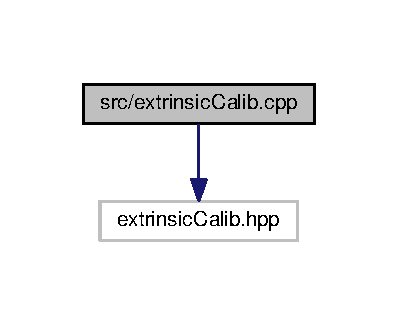
\includegraphics[width=191pt]{extrinsicCalib_8cpp__incl}
\end{center}
\end{figure}
\subsection*{Macros}
\begin{DoxyCompactItemize}
\item 
\#define \hyperlink{extrinsicCalib_8cpp_a588fdde889749bd17e99a8daf595ed57}{D\+I\+S\+T\+\_\+\+C\+O\+E\+F\+F\+S\+\_\+\+D\+E\+F\+A\+U\+LT}
\end{DoxyCompactItemize}
\subsection*{Functions}
\begin{DoxyCompactItemize}
\item 
void \hyperlink{extrinsicCalib_8cpp_a93131970ac4c0e657309ebd9e216f9ee}{write\+Pts2\+C\+SV} (std\+::string file\+\_\+path, std\+::vector$<$ cv\+::\+Point2f $>$ \&img\+\_\+points)
\item 
void \hyperlink{extrinsicCalib_8cpp_adf527c067b4e8a3172c2b9d404aadc08}{read\+Pts\+From\+C\+SV} (std\+::string file\+\_\+path, std\+::vector$<$ cv\+::\+Point2f $>$ \&img\+\_\+points)
\item 
bool \hyperlink{extrinsicCalib_8cpp_a1ee829d0a0e05af2d8888be5e78b457c}{my\+\_\+extrinsic\+Calib} (const cv\+::\+Mat \&img\+\_\+in, std\+::vector$<$ cv\+::\+Point3f $>$ object\+\_\+points, const cv\+::\+Mat \&camera\+\_\+matrix, cv\+::\+Mat \&rvec, cv\+::\+Mat \&tvec, const std\+::string \&config\+\_\+folder)
\item 
void \hyperlink{extrinsicCalib_8cpp_ab271f0495d7510ec99bba8c78254aac4}{my\+\_\+image\+Undistort} (const cv\+::\+Mat \&img\+\_\+in, cv\+::\+Mat \&img\+\_\+out, const cv\+::\+Mat \&cam\+\_\+matrix, const cv\+::\+Mat \&dist\+\_\+coeffs, const std\+::string \&config\+\_\+folder)
\item 
void \hyperlink{extrinsicCalib_8cpp_a48abeda23404e75a75ac77fae135e010}{my\+\_\+find\+Plane\+Transform} (const cv\+::\+Mat \&cam\+\_\+matrix, const cv\+::\+Mat \&rvec, const cv\+::\+Mat \&tvec, const std\+::vector$<$ cv\+::\+Point3f $>$ \&object\+\_\+points\+\_\+plane, const std\+::vector$<$ cv\+::\+Point2f $>$ \&dest\+\_\+image\+\_\+points\+\_\+plane, cv\+::\+Mat \&plane\+\_\+transf, const std\+::string \&config\+\_\+folder)
\item 
void \hyperlink{extrinsicCalib_8cpp_a660d426d048ff9a6ea0076a34ebde64e}{my\+\_\+unwarp} (const cv\+::\+Mat \&img\+\_\+in, cv\+::\+Mat \&img\+\_\+out, const cv\+::\+Mat \&transf, const std\+::string \&config\+\_\+folder)
\end{DoxyCompactItemize}


\subsection{Macro Definition Documentation}
\index{extrinsic\+Calib.\+cpp@{extrinsic\+Calib.\+cpp}!D\+I\+S\+T\+\_\+\+C\+O\+E\+F\+F\+S\+\_\+\+D\+E\+F\+A\+U\+LT@{D\+I\+S\+T\+\_\+\+C\+O\+E\+F\+F\+S\+\_\+\+D\+E\+F\+A\+U\+LT}}
\index{D\+I\+S\+T\+\_\+\+C\+O\+E\+F\+F\+S\+\_\+\+D\+E\+F\+A\+U\+LT@{D\+I\+S\+T\+\_\+\+C\+O\+E\+F\+F\+S\+\_\+\+D\+E\+F\+A\+U\+LT}!extrinsic\+Calib.\+cpp@{extrinsic\+Calib.\+cpp}}
\subsubsection[{\texorpdfstring{D\+I\+S\+T\+\_\+\+C\+O\+E\+F\+F\+S\+\_\+\+D\+E\+F\+A\+U\+LT}{DIST_COEFFS_DEFAULT}}]{\setlength{\rightskip}{0pt plus 5cm}\#define D\+I\+S\+T\+\_\+\+C\+O\+E\+F\+F\+S\+\_\+\+D\+E\+F\+A\+U\+LT}\hypertarget{extrinsicCalib_8cpp_a588fdde889749bd17e99a8daf595ed57}{}\label{extrinsicCalib_8cpp_a588fdde889749bd17e99a8daf595ed57}
Flag to determine dist\+\_\+coeffs values. If def -\/$>$ dist\+\_\+coeffs = \mbox{[}0,0,0,0,0\mbox{]} 

\subsection{Function Documentation}
\index{extrinsic\+Calib.\+cpp@{extrinsic\+Calib.\+cpp}!my\+\_\+extrinsic\+Calib@{my\+\_\+extrinsic\+Calib}}
\index{my\+\_\+extrinsic\+Calib@{my\+\_\+extrinsic\+Calib}!extrinsic\+Calib.\+cpp@{extrinsic\+Calib.\+cpp}}
\subsubsection[{\texorpdfstring{my\+\_\+extrinsic\+Calib(const cv\+::\+Mat \&img\+\_\+in, std\+::vector$<$ cv\+::\+Point3f $>$ object\+\_\+points, const cv\+::\+Mat \&camera\+\_\+matrix, cv\+::\+Mat \&rvec, cv\+::\+Mat \&tvec, const std\+::string \&config\+\_\+folder)}{my_extrinsicCalib(const cv::Mat &img_in, std::vector< cv::Point3f > object_points, const cv::Mat &camera_matrix, cv::Mat &rvec, cv::Mat &tvec, const std::string &config_folder)}}]{\setlength{\rightskip}{0pt plus 5cm}bool my\+\_\+extrinsic\+Calib (
\begin{DoxyParamCaption}
\item[{const cv\+::\+Mat \&}]{img\+\_\+in, }
\item[{std\+::vector$<$ cv\+::\+Point3f $>$}]{object\+\_\+points, }
\item[{const cv\+::\+Mat \&}]{camera\+\_\+matrix, }
\item[{cv\+::\+Mat \&}]{rvec, }
\item[{cv\+::\+Mat \&}]{tvec, }
\item[{const std\+::string \&}]{config\+\_\+folder}
\end{DoxyParamCaption}
)}\hypertarget{extrinsicCalib_8cpp_a1ee829d0a0e05af2d8888be5e78b457c}{}\label{extrinsicCalib_8cpp_a1ee829d0a0e05af2d8888be5e78b457c}
\char`\"{}\+Mask\char`\"{} for extrinsic\+Calib. For more info look in \hyperlink{namespacestudent_a6103f938ce28f8820c48c089d5f95098}{student\+::extrinsic\+Calib} docs. \index{extrinsic\+Calib.\+cpp@{extrinsic\+Calib.\+cpp}!my\+\_\+find\+Plane\+Transform@{my\+\_\+find\+Plane\+Transform}}
\index{my\+\_\+find\+Plane\+Transform@{my\+\_\+find\+Plane\+Transform}!extrinsic\+Calib.\+cpp@{extrinsic\+Calib.\+cpp}}
\subsubsection[{\texorpdfstring{my\+\_\+find\+Plane\+Transform(const cv\+::\+Mat \&cam\+\_\+matrix, const cv\+::\+Mat \&rvec, const cv\+::\+Mat \&tvec, const std\+::vector$<$ cv\+::\+Point3f $>$ \&object\+\_\+points\+\_\+plane, const std\+::vector$<$ cv\+::\+Point2f $>$ \&dest\+\_\+image\+\_\+points\+\_\+plane, cv\+::\+Mat \&plane\+\_\+transf, const std\+::string \&config\+\_\+folder)}{my_findPlaneTransform(const cv::Mat &cam_matrix, const cv::Mat &rvec, const cv::Mat &tvec, const std::vector< cv::Point3f > &object_points_plane, const std::vector< cv::Point2f > &dest_image_points_plane, cv::Mat &plane_transf, const std::string &config_folder)}}]{\setlength{\rightskip}{0pt plus 5cm}void my\+\_\+find\+Plane\+Transform (
\begin{DoxyParamCaption}
\item[{const cv\+::\+Mat \&}]{cam\+\_\+matrix, }
\item[{const cv\+::\+Mat \&}]{rvec, }
\item[{const cv\+::\+Mat \&}]{tvec, }
\item[{const std\+::vector$<$ cv\+::\+Point3f $>$ \&}]{object\+\_\+points\+\_\+plane, }
\item[{const std\+::vector$<$ cv\+::\+Point2f $>$ \&}]{dest\+\_\+image\+\_\+points\+\_\+plane, }
\item[{cv\+::\+Mat \&}]{plane\+\_\+transf, }
\item[{const std\+::string \&}]{config\+\_\+folder}
\end{DoxyParamCaption}
)}\hypertarget{extrinsicCalib_8cpp_a48abeda23404e75a75ac77fae135e010}{}\label{extrinsicCalib_8cpp_a48abeda23404e75a75ac77fae135e010}
\char`\"{}\+Mask\char`\"{} for find\+Plane\+Transform. For more info look in \hyperlink{namespacestudent_a528d33658d0d4d982a46f18b7abb4a70}{student\+::find\+Plane\+Transform} docs. \index{extrinsic\+Calib.\+cpp@{extrinsic\+Calib.\+cpp}!my\+\_\+image\+Undistort@{my\+\_\+image\+Undistort}}
\index{my\+\_\+image\+Undistort@{my\+\_\+image\+Undistort}!extrinsic\+Calib.\+cpp@{extrinsic\+Calib.\+cpp}}
\subsubsection[{\texorpdfstring{my\+\_\+image\+Undistort(const cv\+::\+Mat \&img\+\_\+in, cv\+::\+Mat \&img\+\_\+out, const cv\+::\+Mat \&cam\+\_\+matrix, const cv\+::\+Mat \&dist\+\_\+coeffs, const std\+::string \&config\+\_\+folder)}{my_imageUndistort(const cv::Mat &img_in, cv::Mat &img_out, const cv::Mat &cam_matrix, const cv::Mat &dist_coeffs, const std::string &config_folder)}}]{\setlength{\rightskip}{0pt plus 5cm}void my\+\_\+image\+Undistort (
\begin{DoxyParamCaption}
\item[{const cv\+::\+Mat \&}]{img\+\_\+in, }
\item[{cv\+::\+Mat \&}]{img\+\_\+out, }
\item[{const cv\+::\+Mat \&}]{cam\+\_\+matrix, }
\item[{const cv\+::\+Mat \&}]{dist\+\_\+coeffs, }
\item[{const std\+::string \&}]{config\+\_\+folder}
\end{DoxyParamCaption}
)}\hypertarget{extrinsicCalib_8cpp_ab271f0495d7510ec99bba8c78254aac4}{}\label{extrinsicCalib_8cpp_ab271f0495d7510ec99bba8c78254aac4}
\char`\"{}\+Mask\char`\"{} for image\+Undistort. For more info look in \hyperlink{namespacestudent_aceb2a29362b8223a9d3601d9496e1c98}{student\+::image\+Undistort} docs. \index{extrinsic\+Calib.\+cpp@{extrinsic\+Calib.\+cpp}!my\+\_\+unwarp@{my\+\_\+unwarp}}
\index{my\+\_\+unwarp@{my\+\_\+unwarp}!extrinsic\+Calib.\+cpp@{extrinsic\+Calib.\+cpp}}
\subsubsection[{\texorpdfstring{my\+\_\+unwarp(const cv\+::\+Mat \&img\+\_\+in, cv\+::\+Mat \&img\+\_\+out, const cv\+::\+Mat \&transf, const std\+::string \&config\+\_\+folder)}{my_unwarp(const cv::Mat &img_in, cv::Mat &img_out, const cv::Mat &transf, const std::string &config_folder)}}]{\setlength{\rightskip}{0pt plus 5cm}void my\+\_\+unwarp (
\begin{DoxyParamCaption}
\item[{const cv\+::\+Mat \&}]{img\+\_\+in, }
\item[{cv\+::\+Mat \&}]{img\+\_\+out, }
\item[{const cv\+::\+Mat \&}]{transf, }
\item[{const std\+::string \&}]{config\+\_\+folder}
\end{DoxyParamCaption}
)}\hypertarget{extrinsicCalib_8cpp_a660d426d048ff9a6ea0076a34ebde64e}{}\label{extrinsicCalib_8cpp_a660d426d048ff9a6ea0076a34ebde64e}
\char`\"{}\+Mask\char`\"{} for unwarp. For more info look in \hyperlink{namespacestudent_a6b8caf348979f55e58a75193233c219d}{student\+::unwarp} docs. \index{extrinsic\+Calib.\+cpp@{extrinsic\+Calib.\+cpp}!read\+Pts\+From\+C\+SV@{read\+Pts\+From\+C\+SV}}
\index{read\+Pts\+From\+C\+SV@{read\+Pts\+From\+C\+SV}!extrinsic\+Calib.\+cpp@{extrinsic\+Calib.\+cpp}}
\subsubsection[{\texorpdfstring{read\+Pts\+From\+C\+S\+V(std\+::string file\+\_\+path, std\+::vector$<$ cv\+::\+Point2f $>$ \&img\+\_\+points)}{readPtsFromCSV(std::string file_path, std::vector< cv::Point2f > &img_points)}}]{\setlength{\rightskip}{0pt plus 5cm}void read\+Pts\+From\+C\+SV (
\begin{DoxyParamCaption}
\item[{std\+::string}]{file\+\_\+path, }
\item[{std\+::vector$<$ cv\+::\+Point2f $>$ \&}]{img\+\_\+points}
\end{DoxyParamCaption}
)}\hypertarget{extrinsicCalib_8cpp_adf527c067b4e8a3172c2b9d404aadc08}{}\label{extrinsicCalib_8cpp_adf527c067b4e8a3172c2b9d404aadc08}
It retrives points coordinates wrote line per line in a csv file. 
\begin{DoxyParams}[1]{Parameters}
\mbox{\tt in}  & {\em file\+\_\+path} & Path to the csv file. \\
\hline
\mbox{\tt out}  & {\em img\+\_\+points} & Vector with the read points. \\
\hline
\end{DoxyParams}
\index{extrinsic\+Calib.\+cpp@{extrinsic\+Calib.\+cpp}!write\+Pts2\+C\+SV@{write\+Pts2\+C\+SV}}
\index{write\+Pts2\+C\+SV@{write\+Pts2\+C\+SV}!extrinsic\+Calib.\+cpp@{extrinsic\+Calib.\+cpp}}
\subsubsection[{\texorpdfstring{write\+Pts2\+C\+S\+V(std\+::string file\+\_\+path, std\+::vector$<$ cv\+::\+Point2f $>$ \&img\+\_\+points)}{writePts2CSV(std::string file_path, std::vector< cv::Point2f > &img_points)}}]{\setlength{\rightskip}{0pt plus 5cm}void write\+Pts2\+C\+SV (
\begin{DoxyParamCaption}
\item[{std\+::string}]{file\+\_\+path, }
\item[{std\+::vector$<$ cv\+::\+Point2f $>$ \&}]{img\+\_\+points}
\end{DoxyParamCaption}
)}\hypertarget{extrinsicCalib_8cpp_a93131970ac4c0e657309ebd9e216f9ee}{}\label{extrinsicCalib_8cpp_a93131970ac4c0e657309ebd9e216f9ee}
It writes points coordinates line per line in a csv file. 
\begin{DoxyParams}[1]{Parameters}
\mbox{\tt in}  & {\em file\+\_\+path} & Path to the csv file. \\
\hline
\mbox{\tt in}  & {\em img\+\_\+points} & Vector with the points. \\
\hline
\end{DoxyParams}

\hypertarget{imageManager_8cpp}{}\section{src/image\+Manager.cpp File Reference}
\label{imageManager_8cpp}\index{src/image\+Manager.\+cpp@{src/image\+Manager.\+cpp}}
{\ttfamily \#include \char`\"{}image\+Manager.\+hpp\char`\"{}}\\*
Include dependency graph for image\+Manager.\+cpp\+:\nopagebreak
\begin{figure}[H]
\begin{center}
\leavevmode
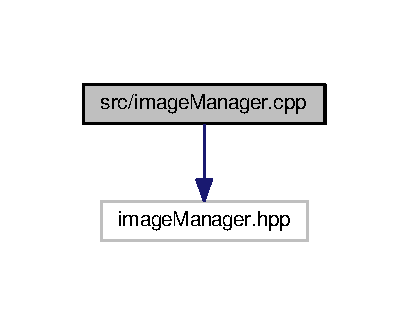
\includegraphics[width=196pt]{imageManager_8cpp__incl}
\end{center}
\end{figure}
\subsection*{Functions}
\begin{DoxyCompactItemize}
\item 
void \hyperlink{imageManager_8cpp_abbb87d0a3860e19ef99e34cd90fbcd3f}{my\+\_\+load\+Image} (cv\+::\+Mat \&img\+\_\+out, const std\+::string \&config\+\_\+folder)
\item 
void \hyperlink{imageManager_8cpp_a4bfa336d36801141879db67e9cf83c0a}{my\+\_\+generic\+Image\+Listener} (const cv\+::\+Mat \&img\+\_\+in, std\+::string topic, const std\+::string \&config\+\_\+folder)
\end{DoxyCompactItemize}


\subsection{Function Documentation}
\index{image\+Manager.\+cpp@{image\+Manager.\+cpp}!my\+\_\+generic\+Image\+Listener@{my\+\_\+generic\+Image\+Listener}}
\index{my\+\_\+generic\+Image\+Listener@{my\+\_\+generic\+Image\+Listener}!image\+Manager.\+cpp@{image\+Manager.\+cpp}}
\subsubsection[{\texorpdfstring{my\+\_\+generic\+Image\+Listener(const cv\+::\+Mat \&img\+\_\+in, std\+::string topic, const std\+::string \&config\+\_\+folder)}{my_genericImageListener(const cv::Mat &img_in, std::string topic, const std::string &config_folder)}}]{\setlength{\rightskip}{0pt plus 5cm}void my\+\_\+generic\+Image\+Listener (
\begin{DoxyParamCaption}
\item[{const cv\+::\+Mat \&}]{img\+\_\+in, }
\item[{std\+::string}]{topic, }
\item[{const std\+::string \&}]{config\+\_\+folder}
\end{DoxyParamCaption}
)}\hypertarget{imageManager_8cpp_a4bfa336d36801141879db67e9cf83c0a}{}\label{imageManager_8cpp_a4bfa336d36801141879db67e9cf83c0a}
\char`\"{}\+Mask\char`\"{} for generic\+Image\+Listener. For more info look in \hyperlink{namespacestudent_a3b726e7af03a643c06dcde23057a82ea}{student\+::generic\+Image\+Listener} docs. Useful for saving chessboard pictures on which to perform the camera calibration. \index{image\+Manager.\+cpp@{image\+Manager.\+cpp}!my\+\_\+load\+Image@{my\+\_\+load\+Image}}
\index{my\+\_\+load\+Image@{my\+\_\+load\+Image}!image\+Manager.\+cpp@{image\+Manager.\+cpp}}
\subsubsection[{\texorpdfstring{my\+\_\+load\+Image(cv\+::\+Mat \&img\+\_\+out, const std\+::string \&config\+\_\+folder)}{my_loadImage(cv::Mat &img_out, const std::string &config_folder)}}]{\setlength{\rightskip}{0pt plus 5cm}void my\+\_\+load\+Image (
\begin{DoxyParamCaption}
\item[{cv\+::\+Mat \&}]{img\+\_\+out, }
\item[{const std\+::string \&}]{config\+\_\+folder}
\end{DoxyParamCaption}
)}\hypertarget{imageManager_8cpp_abbb87d0a3860e19ef99e34cd90fbcd3f}{}\label{imageManager_8cpp_abbb87d0a3860e19ef99e34cd90fbcd3f}
\char`\"{}\+Mask\char`\"{} for load\+Image. For more info look in \hyperlink{namespacestudent_a3117c968a47bf95f86bdb813a3b64e56}{student\+::load\+Image} docs. Replace the use of the simulator -\/$>$ useful for testing the shape detection on real picture. 
\hypertarget{mapProcessing_8cpp}{}\section{src/map\+Processing.cpp File Reference}
\label{mapProcessing_8cpp}\index{src/map\+Processing.\+cpp@{src/map\+Processing.\+cpp}}
{\ttfamily \#include \char`\"{}map\+Processing.\+hpp\char`\"{}}\\*
Include dependency graph for map\+Processing.\+cpp\+:\nopagebreak
\begin{figure}[H]
\begin{center}
\leavevmode
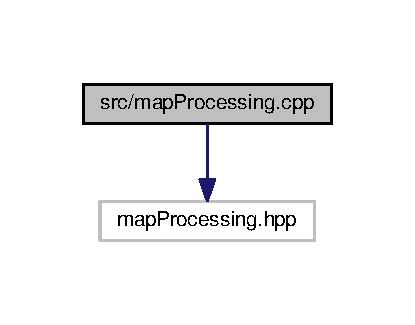
\includegraphics[width=199pt]{mapProcessing_8cpp__incl}
\end{center}
\end{figure}
\subsection*{Macros}
\begin{DoxyCompactItemize}
\item 
\#define \hyperlink{mapProcessing_8cpp_a8a7f485573c16394fc0792a66bd02c7a}{A\+N\+G\+LE}~90
\item 
\#define \hyperlink{mapProcessing_8cpp_a891296e8a86925e86dd7d2b270c95871}{X\+\_\+\+F\+L\+IP}~false
\item 
\#define \hyperlink{mapProcessing_8cpp_abebd71c1327d2cadd1de7f3989995338}{Y\+\_\+\+F\+L\+IP}~true
\end{DoxyCompactItemize}
\subsection*{Functions}
\begin{DoxyCompactItemize}
\item 
void \hyperlink{mapProcessing_8cpp_a883e6e6ffba02aa8042022efc6e44adf}{remove\+Noise} (cv\+::\+Mat \&mask)
\item 
void \hyperlink{mapProcessing_8cpp_a017a9b7bedb7eec7b62d9339ff2dae5e}{get\+Approx\+Mask\+Contours} (cv\+::\+Mat \&mask, int dist\+\_\+accuracy, const double scale, std\+::vector$<$ Polygon $>$ \&obj\+\_\+contour\+\_\+list)
\item 
bool \hyperlink{mapProcessing_8cpp_a2e9e3940aeb6118fba848bca7d58e179}{get\+Robot} (const cv\+::\+Mat \&hsv\+\_\+img, const double scale, Polygon \&triangle)
\item 
double \hyperlink{mapProcessing_8cpp_abd6a9dabd3cd316d9e00f5d907b1256c}{get\+Triangle\+Radius} (const cv\+::\+Mat \&hsv\+\_\+img, const double scale)
\item 
void \hyperlink{mapProcessing_8cpp_a17d6433f7da39cb4562c1f6c8dc104ba}{offset\+Obstacles} (double offset, std\+::vector$<$ Polygon $>$ \&obstacles\+\_\+list, const double scale)
\item 
void \hyperlink{mapProcessing_8cpp_afc86389fd87c790523b63d42edbe7564}{get\+Obstacles} (const cv\+::\+Mat \&hsv\+\_\+img, const double scale, std\+::vector$<$ Polygon $>$ \&obstacles\+\_\+list)
\item 
void \hyperlink{mapProcessing_8cpp_a03dfaf7cb1df6ee0ebfa1b2e37bd4c20}{get\+Template\+Imgs} (std\+::vector$<$ std\+::pair$<$ int, cv\+::\+Mat $>$$>$ \&template\+\_\+img\+\_\+list)
\item 
void \hyperlink{mapProcessing_8cpp_a98d90ce213a536d6c50b58246bee3928}{get\+Edited\+R\+OI} (cv\+::\+Mat \&orig\+\_\+\+R\+OI, const double angle, bool flag\+\_\+x\+\_\+flip, bool flag\+\_\+y\+\_\+flip, cv\+::\+Mat \&edited\+\_\+\+R\+OI)
\item 
void \hyperlink{mapProcessing_8cpp_af800f64ebf6cfe01f6c2c220ecfeb305}{get\+T\+M\+Digit} (cv\+::\+Mat \&edited\+\_\+\+R\+OI, std\+::vector$<$ std\+::pair$<$ int, cv\+::\+Mat $>$$>$ \&template\+\_\+img\+\_\+list, int \&victim\+\_\+id)
\item 
int \hyperlink{mapProcessing_8cpp_a62195cf4f3f756fed379cbc39c178027}{get\+Victim\+ID} (const cv\+::\+Mat \&hsv\+\_\+img, const cv\+::\+Mat \&mask, const double scale, const Polygon \&victim\+\_\+contour, std\+::vector$<$ std\+::pair$<$ int, cv\+::\+Mat $>$$>$ \&template\+\_\+images)
\item 
void \hyperlink{mapProcessing_8cpp_adbfc86d4dbb2c1a18b57542a5b983893}{get\+Victims\+And\+Gate} (const cv\+::\+Mat \&hsv\+\_\+img, const double scale, std\+::vector$<$ std\+::pair$<$ int, Polygon $>$$>$ \&victims\+\_\+list, Polygon \&gate)
\item 
void \hyperlink{mapProcessing_8cpp_a0fc4f08db177646fe611eee737434b05}{get\+Orientation} (Polygon \&triangle, double \&baricenter\+\_\+x, double \&baricenter\+\_\+y, double \&theta)
\item 
bool \hyperlink{mapProcessing_8cpp_ace488fd56a8a7af5f51cd0e2d0e1f64e}{my\+\_\+process\+Map} (const cv\+::\+Mat \&img\+\_\+in, const double scale, std\+::vector$<$ Polygon $>$ \&obstacles\+\_\+list, std\+::vector$<$ std\+::pair$<$ int, Polygon $>$$>$ \&victims\+\_\+list, Polygon \&gate, const std\+::string \&config\+\_\+folder)
\item 
bool \hyperlink{mapProcessing_8cpp_a7ef6c7ca3985fcd74c63ddd4f00f2f04}{my\+\_\+find\+Robot} (const cv\+::\+Mat \&img\+\_\+in, const double scale, Polygon \&triangle, double \&x, double \&y, double \&theta, const std\+::string \&config\+\_\+folder)
\end{DoxyCompactItemize}


\subsection{Macro Definition Documentation}
\index{map\+Processing.\+cpp@{map\+Processing.\+cpp}!A\+N\+G\+LE@{A\+N\+G\+LE}}
\index{A\+N\+G\+LE@{A\+N\+G\+LE}!map\+Processing.\+cpp@{map\+Processing.\+cpp}}
\subsubsection[{\texorpdfstring{A\+N\+G\+LE}{ANGLE}}]{\setlength{\rightskip}{0pt plus 5cm}\#define A\+N\+G\+LE~90}\hypertarget{mapProcessing_8cpp_a8a7f485573c16394fc0792a66bd02c7a}{}\label{mapProcessing_8cpp_a8a7f485573c16394fc0792a66bd02c7a}
Rotation angle to apply to the R\+OI of a detected digit. \index{map\+Processing.\+cpp@{map\+Processing.\+cpp}!X\+\_\+\+F\+L\+IP@{X\+\_\+\+F\+L\+IP}}
\index{X\+\_\+\+F\+L\+IP@{X\+\_\+\+F\+L\+IP}!map\+Processing.\+cpp@{map\+Processing.\+cpp}}
\subsubsection[{\texorpdfstring{X\+\_\+\+F\+L\+IP}{X_FLIP}}]{\setlength{\rightskip}{0pt plus 5cm}\#define X\+\_\+\+F\+L\+IP~false}\hypertarget{mapProcessing_8cpp_a891296e8a86925e86dd7d2b270c95871}{}\label{mapProcessing_8cpp_a891296e8a86925e86dd7d2b270c95871}
True if the R\+OI has to be flipped on the x axis, false otherwise. \index{map\+Processing.\+cpp@{map\+Processing.\+cpp}!Y\+\_\+\+F\+L\+IP@{Y\+\_\+\+F\+L\+IP}}
\index{Y\+\_\+\+F\+L\+IP@{Y\+\_\+\+F\+L\+IP}!map\+Processing.\+cpp@{map\+Processing.\+cpp}}
\subsubsection[{\texorpdfstring{Y\+\_\+\+F\+L\+IP}{Y_FLIP}}]{\setlength{\rightskip}{0pt plus 5cm}\#define Y\+\_\+\+F\+L\+IP~true}\hypertarget{mapProcessing_8cpp_abebd71c1327d2cadd1de7f3989995338}{}\label{mapProcessing_8cpp_abebd71c1327d2cadd1de7f3989995338}
True if the R\+OI has to be flipped on the y axis, false otherwise. 

\subsection{Function Documentation}
\index{map\+Processing.\+cpp@{map\+Processing.\+cpp}!get\+Approx\+Mask\+Contours@{get\+Approx\+Mask\+Contours}}
\index{get\+Approx\+Mask\+Contours@{get\+Approx\+Mask\+Contours}!map\+Processing.\+cpp@{map\+Processing.\+cpp}}
\subsubsection[{\texorpdfstring{get\+Approx\+Mask\+Contours(cv\+::\+Mat \&mask, int dist\+\_\+accuracy, const double scale, std\+::vector$<$ Polygon $>$ \&obj\+\_\+contour\+\_\+list)}{getApproxMaskContours(cv::Mat &mask, int dist_accuracy, const double scale, std::vector< Polygon > &obj_contour_list)}}]{\setlength{\rightskip}{0pt plus 5cm}void get\+Approx\+Mask\+Contours (
\begin{DoxyParamCaption}
\item[{cv\+::\+Mat \&}]{mask, }
\item[{int}]{dist\+\_\+accuracy, }
\item[{const double}]{scale, }
\item[{std\+::vector$<$ Polygon $>$ \&}]{obj\+\_\+contour\+\_\+list}
\end{DoxyParamCaption}
)}\hypertarget{mapProcessing_8cpp_a017a9b7bedb7eec7b62d9339ff2dae5e}{}\label{mapProcessing_8cpp_a017a9b7bedb7eec7b62d9339ff2dae5e}
Retrieves the approximated contours of mask. 
\begin{DoxyParams}[1]{Parameters}
\mbox{\tt in}  & {\em mask} & Denoised bitmap mask matrix for a certain color. \\
\hline
\mbox{\tt in}  & {\em dist\+\_\+accuracy} & Max distance between the original curve and its approximation. \\
\hline
\mbox{\tt in}  & {\em scale} & Scale of the arena (1px/scale = X meters). \\
\hline
\mbox{\tt out}  & {\em obj\+\_\+contour\+\_\+list} & List of objs contours (vertex in meters). \\
\hline
\end{DoxyParams}
\index{map\+Processing.\+cpp@{map\+Processing.\+cpp}!get\+Edited\+R\+OI@{get\+Edited\+R\+OI}}
\index{get\+Edited\+R\+OI@{get\+Edited\+R\+OI}!map\+Processing.\+cpp@{map\+Processing.\+cpp}}
\subsubsection[{\texorpdfstring{get\+Edited\+R\+O\+I(cv\+::\+Mat \&orig\+\_\+\+R\+O\+I, const double angle, bool flag\+\_\+x\+\_\+flip, bool flag\+\_\+y\+\_\+flip, cv\+::\+Mat \&edited\+\_\+\+R\+O\+I)}{getEditedROI(cv::Mat &orig_ROI, const double angle, bool flag_x_flip, bool flag_y_flip, cv::Mat &edited_ROI)}}]{\setlength{\rightskip}{0pt plus 5cm}void get\+Edited\+R\+OI (
\begin{DoxyParamCaption}
\item[{cv\+::\+Mat \&}]{orig\+\_\+\+R\+OI, }
\item[{const double}]{angle, }
\item[{bool}]{flag\+\_\+x\+\_\+flip, }
\item[{bool}]{flag\+\_\+y\+\_\+flip, }
\item[{cv\+::\+Mat \&}]{edited\+\_\+\+R\+OI}
\end{DoxyParamCaption}
)}\hypertarget{mapProcessing_8cpp_a98d90ce213a536d6c50b58246bee3928}{}\label{mapProcessing_8cpp_a98d90ce213a536d6c50b58246bee3928}
Assuming all victims have been rotated and flipped in the same known way, it applies a series of modification in order to make orig\+\_\+\+R\+OI readable/recognizable. 
\begin{DoxyParams}[1]{Parameters}
\mbox{\tt in}  & {\em orig\+\_\+\+R\+OI} & Original R\+OI. \\
\hline
\mbox{\tt in}  & {\em angle} & Angle of rotation. \\
\hline
\mbox{\tt in}  & {\em flag\+\_\+x\+\_\+flip} & Flag indicating whether the R\+OI has to be flipped on the x-\/axis. \\
\hline
\mbox{\tt in}  & {\em flag\+\_\+y\+\_\+flip} & Flag indicating whether the R\+OI has to be flipped on the y-\/axis. \\
\hline
\mbox{\tt out}  & {\em edited\+\_\+\+R\+OI} & Readable/recognizable R\+OI. \\
\hline
\end{DoxyParams}
\index{map\+Processing.\+cpp@{map\+Processing.\+cpp}!get\+Obstacles@{get\+Obstacles}}
\index{get\+Obstacles@{get\+Obstacles}!map\+Processing.\+cpp@{map\+Processing.\+cpp}}
\subsubsection[{\texorpdfstring{get\+Obstacles(const cv\+::\+Mat \&hsv\+\_\+img, const double scale, std\+::vector$<$ Polygon $>$ \&obstacles\+\_\+list)}{getObstacles(const cv::Mat &hsv_img, const double scale, std::vector< Polygon > &obstacles_list)}}]{\setlength{\rightskip}{0pt plus 5cm}void get\+Obstacles (
\begin{DoxyParamCaption}
\item[{const cv\+::\+Mat \&}]{hsv\+\_\+img, }
\item[{const double}]{scale, }
\item[{std\+::vector$<$ Polygon $>$ \&}]{obstacles\+\_\+list}
\end{DoxyParamCaption}
)}\hypertarget{mapProcessing_8cpp_afc86389fd87c790523b63d42edbe7564}{}\label{mapProcessing_8cpp_afc86389fd87c790523b63d42edbe7564}
Retrieves the obstacles. 
\begin{DoxyParams}[1]{Parameters}
\mbox{\tt in}  & {\em hsv\+\_\+img} & Original img in hsv space. \\
\hline
\mbox{\tt in}  & {\em scale} & Scale of the arena (1px/scale = X meters). \\
\hline
\mbox{\tt out}  & {\em obstacles\+\_\+list} & List of obstacles (vertex in meters). \\
\hline
\end{DoxyParams}
\index{map\+Processing.\+cpp@{map\+Processing.\+cpp}!get\+Orientation@{get\+Orientation}}
\index{get\+Orientation@{get\+Orientation}!map\+Processing.\+cpp@{map\+Processing.\+cpp}}
\subsubsection[{\texorpdfstring{get\+Orientation(\+Polygon \&triangle, double \&baricenter\+\_\+x, double \&baricenter\+\_\+y, double \&theta)}{getOrientation(Polygon &triangle, double &baricenter_x, double &baricenter_y, double &theta)}}]{\setlength{\rightskip}{0pt plus 5cm}void get\+Orientation (
\begin{DoxyParamCaption}
\item[{Polygon \&}]{triangle, }
\item[{double \&}]{baricenter\+\_\+x, }
\item[{double \&}]{baricenter\+\_\+y, }
\item[{double \&}]{theta}
\end{DoxyParamCaption}
)}\hypertarget{mapProcessing_8cpp_a0fc4f08db177646fe611eee737434b05}{}\label{mapProcessing_8cpp_a0fc4f08db177646fe611eee737434b05}
Retrieves the robot/trianlge\textquotesingle{}s orientation. 
\begin{DoxyParams}[1]{Parameters}
\mbox{\tt in}  & {\em triangle} & Robot/triangle polygon. \\
\hline
\mbox{\tt in}  & {\em baricenter\+\_\+x} & Baricenter\textquotesingle{}s x coordinate. \\
\hline
\mbox{\tt in}  & {\em baricenter\+\_\+y} & Baricenter\textquotesingle{}s y coordinate. \\
\hline
\mbox{\tt out}  & {\em theta} & Robot/triangle\textquotesingle{}s orientation. \\
\hline
\end{DoxyParams}
\index{map\+Processing.\+cpp@{map\+Processing.\+cpp}!get\+Robot@{get\+Robot}}
\index{get\+Robot@{get\+Robot}!map\+Processing.\+cpp@{map\+Processing.\+cpp}}
\subsubsection[{\texorpdfstring{get\+Robot(const cv\+::\+Mat \&hsv\+\_\+img, const double scale, Polygon \&triangle)}{getRobot(const cv::Mat &hsv_img, const double scale, Polygon &triangle)}}]{\setlength{\rightskip}{0pt plus 5cm}bool get\+Robot (
\begin{DoxyParamCaption}
\item[{const cv\+::\+Mat \&}]{hsv\+\_\+img, }
\item[{const double}]{scale, }
\item[{Polygon \&}]{triangle}
\end{DoxyParamCaption}
)}\hypertarget{mapProcessing_8cpp_a2e9e3940aeb6118fba848bca7d58e179}{}\label{mapProcessing_8cpp_a2e9e3940aeb6118fba848bca7d58e179}
Retrieves the robot/triangle. 
\begin{DoxyParams}[1]{Parameters}
\mbox{\tt in}  & {\em hsv\+\_\+img} & Original img in hsv space. \\
\hline
\mbox{\tt in}  & {\em scale} & Scale of the arena (1px/scale = X meters). \\
\hline
\mbox{\tt out}  & {\em triangle} & Robot/triangle polygon. \\
\hline
\end{DoxyParams}
\index{map\+Processing.\+cpp@{map\+Processing.\+cpp}!get\+Template\+Imgs@{get\+Template\+Imgs}}
\index{get\+Template\+Imgs@{get\+Template\+Imgs}!map\+Processing.\+cpp@{map\+Processing.\+cpp}}
\subsubsection[{\texorpdfstring{get\+Template\+Imgs(std\+::vector$<$ std\+::pair$<$ int, cv\+::\+Mat $>$$>$ \&template\+\_\+img\+\_\+list)}{getTemplateImgs(std::vector< std::pair< int, cv::Mat >> &template_img_list)}}]{\setlength{\rightskip}{0pt plus 5cm}void get\+Template\+Imgs (
\begin{DoxyParamCaption}
\item[{std\+::vector$<$ std\+::pair$<$ int, cv\+::\+Mat $>$$>$ \&}]{template\+\_\+img\+\_\+list}
\end{DoxyParamCaption}
)}\hypertarget{mapProcessing_8cpp_a03dfaf7cb1df6ee0ebfa1b2e37bd4c20}{}\label{mapProcessing_8cpp_a03dfaf7cb1df6ee0ebfa1b2e37bd4c20}
Support function which retrives all the template images from src/template\+\_\+images. 
\begin{DoxyParams}[1]{Parameters}
\mbox{\tt out}  & {\em template\+\_\+img\+\_\+list} & Vector of pairs $<$represented id, template image$>$. \\
\hline
\end{DoxyParams}
\index{map\+Processing.\+cpp@{map\+Processing.\+cpp}!get\+T\+M\+Digit@{get\+T\+M\+Digit}}
\index{get\+T\+M\+Digit@{get\+T\+M\+Digit}!map\+Processing.\+cpp@{map\+Processing.\+cpp}}
\subsubsection[{\texorpdfstring{get\+T\+M\+Digit(cv\+::\+Mat \&edited\+\_\+\+R\+O\+I, std\+::vector$<$ std\+::pair$<$ int, cv\+::\+Mat $>$$>$ \&template\+\_\+img\+\_\+list, int \&victim\+\_\+id)}{getTMDigit(cv::Mat &edited_ROI, std::vector< std::pair< int, cv::Mat >> &template_img_list, int &victim_id)}}]{\setlength{\rightskip}{0pt plus 5cm}void get\+T\+M\+Digit (
\begin{DoxyParamCaption}
\item[{cv\+::\+Mat \&}]{edited\+\_\+\+R\+OI, }
\item[{std\+::vector$<$ std\+::pair$<$ int, cv\+::\+Mat $>$$>$ \&}]{template\+\_\+img\+\_\+list, }
\item[{int \&}]{victim\+\_\+id}
\end{DoxyParamCaption}
)}\hypertarget{mapProcessing_8cpp_af800f64ebf6cfe01f6c2c220ecfeb305}{}\label{mapProcessing_8cpp_af800f64ebf6cfe01f6c2c220ecfeb305}
Retrieves the best matching digit (a.\+k.\+a the victim\textquotesingle{}s id). 
\begin{DoxyParams}[1]{Parameters}
\mbox{\tt in}  & {\em edited\+\_\+\+R\+OI} & Readable/recognizable R\+OI. \\
\hline
\mbox{\tt in}  & {\em template\+\_\+img\+\_\+list} & Vector of pairs $<$represented id, template image$>$. \\
\hline
\mbox{\tt out}  & {\em victim\+\_\+id} & Matched digit in edited\+\_\+\+R\+OI. \\
\hline
\end{DoxyParams}
\index{map\+Processing.\+cpp@{map\+Processing.\+cpp}!get\+Triangle\+Radius@{get\+Triangle\+Radius}}
\index{get\+Triangle\+Radius@{get\+Triangle\+Radius}!map\+Processing.\+cpp@{map\+Processing.\+cpp}}
\subsubsection[{\texorpdfstring{get\+Triangle\+Radius(const cv\+::\+Mat \&hsv\+\_\+img, const double scale)}{getTriangleRadius(const cv::Mat &hsv_img, const double scale)}}]{\setlength{\rightskip}{0pt plus 5cm}double get\+Triangle\+Radius (
\begin{DoxyParamCaption}
\item[{const cv\+::\+Mat \&}]{hsv\+\_\+img, }
\item[{const double}]{scale}
\end{DoxyParamCaption}
)}\hypertarget{mapProcessing_8cpp_abd6a9dabd3cd316d9e00f5d907b1256c}{}\label{mapProcessing_8cpp_abd6a9dabd3cd316d9e00f5d907b1256c}
Retrieves the radius of the circle that circumscribes the triangle. 
\begin{DoxyParams}[1]{Parameters}
\mbox{\tt in}  & {\em hsv\+\_\+img} & Original img in hsv space. \\
\hline
\mbox{\tt in}  & {\em scale} & Scale of the arena (1px/scale = X meters). \\
\hline
\end{DoxyParams}
\begin{DoxyReturn}{Returns}
\mbox{[}double\mbox{]} radius Retrieved radius (in meters). 
\end{DoxyReturn}
\index{map\+Processing.\+cpp@{map\+Processing.\+cpp}!get\+Victim\+ID@{get\+Victim\+ID}}
\index{get\+Victim\+ID@{get\+Victim\+ID}!map\+Processing.\+cpp@{map\+Processing.\+cpp}}
\subsubsection[{\texorpdfstring{get\+Victim\+I\+D(const cv\+::\+Mat \&hsv\+\_\+img, const cv\+::\+Mat \&mask, const double scale, const Polygon \&victim\+\_\+contour, std\+::vector$<$ std\+::pair$<$ int, cv\+::\+Mat $>$$>$ \&template\+\_\+images)}{getVictimID(const cv::Mat &hsv_img, const cv::Mat &mask, const double scale, const Polygon &victim_contour, std::vector< std::pair< int, cv::Mat >> &template_images)}}]{\setlength{\rightskip}{0pt plus 5cm}int get\+Victim\+ID (
\begin{DoxyParamCaption}
\item[{const cv\+::\+Mat \&}]{hsv\+\_\+img, }
\item[{const cv\+::\+Mat \&}]{mask, }
\item[{const double}]{scale, }
\item[{const Polygon \&}]{victim\+\_\+contour, }
\item[{std\+::vector$<$ std\+::pair$<$ int, cv\+::\+Mat $>$$>$ \&}]{template\+\_\+images}
\end{DoxyParamCaption}
)}\hypertarget{mapProcessing_8cpp_a62195cf4f3f756fed379cbc39c178027}{}\label{mapProcessing_8cpp_a62195cf4f3f756fed379cbc39c178027}
Recognize and retrieves the victim\textquotesingle{}s ID by means of tesserract. 
\begin{DoxyParams}[1]{Parameters}
\mbox{\tt in}  & {\em hsv\+\_\+img} & Original image in hsv space. \\
\hline
\mbox{\tt in}  & {\em mask} & Green mask. \\
\hline
\mbox{\tt in}  & {\em scale} & Scale of the arena (1px/scale = X meters). \\
\hline
\mbox{\tt in}  & {\em victim\+\_\+contours} & Victim points which define the contours. \\
\hline
\mbox{\tt in}  & {\em template\+\_\+images} & Vector of template images. \\
\hline
\end{DoxyParams}
\begin{DoxyReturn}{Returns}
\mbox{[}int\mbox{]} victim\+\_\+id The retrieved victim id. 
\end{DoxyReturn}
\index{map\+Processing.\+cpp@{map\+Processing.\+cpp}!get\+Victims\+And\+Gate@{get\+Victims\+And\+Gate}}
\index{get\+Victims\+And\+Gate@{get\+Victims\+And\+Gate}!map\+Processing.\+cpp@{map\+Processing.\+cpp}}
\subsubsection[{\texorpdfstring{get\+Victims\+And\+Gate(const cv\+::\+Mat \&hsv\+\_\+img, const double scale, std\+::vector$<$ std\+::pair$<$ int, Polygon $>$$>$ \&victims\+\_\+list, Polygon \&gate)}{getVictimsAndGate(const cv::Mat &hsv_img, const double scale, std::vector< std::pair< int, Polygon >> &victims_list, Polygon &gate)}}]{\setlength{\rightskip}{0pt plus 5cm}void get\+Victims\+And\+Gate (
\begin{DoxyParamCaption}
\item[{const cv\+::\+Mat \&}]{hsv\+\_\+img, }
\item[{const double}]{scale, }
\item[{std\+::vector$<$ std\+::pair$<$ int, Polygon $>$$>$ \&}]{victims\+\_\+list, }
\item[{Polygon \&}]{gate}
\end{DoxyParamCaption}
)}\hypertarget{mapProcessing_8cpp_adbfc86d4dbb2c1a18b57542a5b983893}{}\label{mapProcessing_8cpp_adbfc86d4dbb2c1a18b57542a5b983893}
Retrieves the victims and the gate. Victims and gate are discriminated by the number of verteces. 
\begin{DoxyParams}[1]{Parameters}
\mbox{\tt in}  & {\em hsv\+\_\+img} & Original img in hsv space. \\
\hline
\mbox{\tt in}  & {\em scale} & Scale of the arena (1px/scale = X meters). \\
\hline
\mbox{\tt out}  & {\em victims\+\_\+list} & List of obstacles. \\
\hline
\mbox{\tt out}  & {\em gate} & Gate polygon. \\
\hline
\end{DoxyParams}
\index{map\+Processing.\+cpp@{map\+Processing.\+cpp}!my\+\_\+find\+Robot@{my\+\_\+find\+Robot}}
\index{my\+\_\+find\+Robot@{my\+\_\+find\+Robot}!map\+Processing.\+cpp@{map\+Processing.\+cpp}}
\subsubsection[{\texorpdfstring{my\+\_\+find\+Robot(const cv\+::\+Mat \&img\+\_\+in, const double scale, Polygon \&triangle, double \&x, double \&y, double \&theta, const std\+::string \&config\+\_\+folder)}{my_findRobot(const cv::Mat &img_in, const double scale, Polygon &triangle, double &x, double &y, double &theta, const std::string &config_folder)}}]{\setlength{\rightskip}{0pt plus 5cm}bool my\+\_\+find\+Robot (
\begin{DoxyParamCaption}
\item[{const cv\+::\+Mat \&}]{img\+\_\+in, }
\item[{const double}]{scale, }
\item[{Polygon \&}]{triangle, }
\item[{double \&}]{x, }
\item[{double \&}]{y, }
\item[{double \&}]{theta, }
\item[{const std\+::string \&}]{config\+\_\+folder}
\end{DoxyParamCaption}
)}\hypertarget{mapProcessing_8cpp_a7ef6c7ca3985fcd74c63ddd4f00f2f04}{}\label{mapProcessing_8cpp_a7ef6c7ca3985fcd74c63ddd4f00f2f04}
\char`\"{}\+Mask\char`\"{} for find\+Robot. For more info look in \hyperlink{namespacestudent_afd56b779672a672e15ac45dc927b8a6b}{student\+::find\+Robot} docs. \index{map\+Processing.\+cpp@{map\+Processing.\+cpp}!my\+\_\+process\+Map@{my\+\_\+process\+Map}}
\index{my\+\_\+process\+Map@{my\+\_\+process\+Map}!map\+Processing.\+cpp@{map\+Processing.\+cpp}}
\subsubsection[{\texorpdfstring{my\+\_\+process\+Map(const cv\+::\+Mat \&img\+\_\+in, const double scale, std\+::vector$<$ Polygon $>$ \&obstacles\+\_\+list, std\+::vector$<$ std\+::pair$<$ int, Polygon $>$$>$ \&victims\+\_\+list, Polygon \&gate, const std\+::string \&config\+\_\+folder)}{my_processMap(const cv::Mat &img_in, const double scale, std::vector< Polygon > &obstacles_list, std::vector< std::pair< int, Polygon >> &victims_list, Polygon &gate, const std::string &config_folder)}}]{\setlength{\rightskip}{0pt plus 5cm}bool my\+\_\+process\+Map (
\begin{DoxyParamCaption}
\item[{const cv\+::\+Mat \&}]{img\+\_\+in, }
\item[{const double}]{scale, }
\item[{std\+::vector$<$ Polygon $>$ \&}]{obstacles\+\_\+list, }
\item[{std\+::vector$<$ std\+::pair$<$ int, Polygon $>$$>$ \&}]{victims\+\_\+list, }
\item[{Polygon \&}]{gate, }
\item[{const std\+::string \&}]{config\+\_\+folder}
\end{DoxyParamCaption}
)}\hypertarget{mapProcessing_8cpp_ace488fd56a8a7af5f51cd0e2d0e1f64e}{}\label{mapProcessing_8cpp_ace488fd56a8a7af5f51cd0e2d0e1f64e}
\char`\"{}\+Mask\char`\"{} for process\+Map. For more info look in \hyperlink{namespacestudent_a684c71c41ce1327ab90152b661ee1e8a}{student\+::process\+Map} docs. \index{map\+Processing.\+cpp@{map\+Processing.\+cpp}!offset\+Obstacles@{offset\+Obstacles}}
\index{offset\+Obstacles@{offset\+Obstacles}!map\+Processing.\+cpp@{map\+Processing.\+cpp}}
\subsubsection[{\texorpdfstring{offset\+Obstacles(double offset, std\+::vector$<$ Polygon $>$ \&obstacles\+\_\+list, const double scale)}{offsetObstacles(double offset, std::vector< Polygon > &obstacles_list, const double scale)}}]{\setlength{\rightskip}{0pt plus 5cm}void offset\+Obstacles (
\begin{DoxyParamCaption}
\item[{double}]{offset, }
\item[{std\+::vector$<$ Polygon $>$ \&}]{obstacles\+\_\+list, }
\item[{const double}]{scale}
\end{DoxyParamCaption}
)}\hypertarget{mapProcessing_8cpp_a17d6433f7da39cb4562c1f6c8dc104ba}{}\label{mapProcessing_8cpp_a17d6433f7da39cb4562c1f6c8dc104ba}
Inflates the obstacles of a list with a given offset by means of Clipper\+Lib. 
\begin{DoxyParams}[1]{Parameters}
\mbox{\tt in}  & {\em offset} & Offset to apply (in meters). \\
\hline
\mbox{\tt in}  & {\em obstacles\+\_\+list} & List of obstacles (vertex in meters). \\
\hline
\mbox{\tt in}  & {\em scale} & Scale of the arena (1px/scale = X meters). \\
\hline
\mbox{\tt out}  & {\em obstacles\+\_\+list} & List of offsetted obstacles (vertex in meters). \\
\hline
\end{DoxyParams}
\index{map\+Processing.\+cpp@{map\+Processing.\+cpp}!remove\+Noise@{remove\+Noise}}
\index{remove\+Noise@{remove\+Noise}!map\+Processing.\+cpp@{map\+Processing.\+cpp}}
\subsubsection[{\texorpdfstring{remove\+Noise(cv\+::\+Mat \&mask)}{removeNoise(cv::Mat &mask)}}]{\setlength{\rightskip}{0pt plus 5cm}void remove\+Noise (
\begin{DoxyParamCaption}
\item[{cv\+::\+Mat \&}]{mask}
\end{DoxyParamCaption}
)}\hypertarget{mapProcessing_8cpp_a883e6e6ffba02aa8042022efc6e44adf}{}\label{mapProcessing_8cpp_a883e6e6ffba02aa8042022efc6e44adf}
Erode and dilate the mask with a 4x4 kernel. 
\begin{DoxyParams}[1]{Parameters}
\mbox{\tt out}  & {\em mask} & Bitmap mask matrix for a certain color. \\
\hline
\end{DoxyParams}

\hypertarget{pathPlanning_8cpp}{}\section{src/path\+Planning.cpp File Reference}
\label{pathPlanning_8cpp}\index{src/path\+Planning.\+cpp@{src/path\+Planning.\+cpp}}
{\ttfamily \#include \char`\"{}path\+Planning.\+hpp\char`\"{}}\\*
Include dependency graph for path\+Planning.\+cpp\+:\nopagebreak
\begin{figure}[H]
\begin{center}
\leavevmode
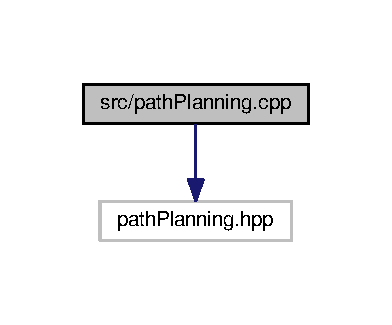
\includegraphics[width=188pt]{pathPlanning_8cpp__incl}
\end{center}
\end{figure}
\subsection*{Macros}
\begin{DoxyCompactItemize}
\item 
\#define \hyperlink{pathPlanning_8cpp_a0e1825ddd7e05b735b28f1137fcaf78e}{M\+I\+S\+S\+I\+O\+N\+\_\+1}
\item 
\#define \hyperlink{pathPlanning_8cpp_a67f9565ee144db95e5394b15e393e539}{N\+\_\+\+P\+TS}~250
\item 
\#define \hyperlink{pathPlanning_8cpp_a3b1076720ba707d01eb86475b2e2529b}{K\+NN}~10
\end{DoxyCompactItemize}
\subsection*{Functions}
\begin{DoxyCompactItemize}
\item 
bool \hyperlink{pathPlanning_8cpp_a30baa5ddb4612336969595f47876c5e1}{sort\+Victims\+By\+ID} (const std\+::pair$<$ int, Point $>$ \&i, const std\+::pair$<$ int, Point $>$ \&j)
\item 
void \hyperlink{pathPlanning_8cpp_a9baab275277a6c78a21be766fa5795c5}{expand\+Obstacle\+List} (const int id, const std\+::vector$<$ std\+::pair$<$ int, Polygon $>$$>$ \&victim\+\_\+list, std\+::vector$<$ Polygon $>$ \&expanded\+\_\+list)
\item 
void \hyperlink{pathPlanning_8cpp_a58433264a5ace17ffe7276ba235fcb98}{create\+Path} (const std\+::vector$<$ curve $>$ \&dubins\+\_\+path, Path \&path)
\item 
float \hyperlink{pathPlanning_8cpp_af1c9a6a9923e46591eabc35b9fa6ed02}{get\+Path\+Distance} (const std\+::vector$<$ Point $>$ path)
\item 
bool \hyperlink{pathPlanning_8cpp_a1167a1806905a9b2df3591f4e3821dca}{my\+\_\+plan\+Path} (const Polygon \&borders, const std\+::vector$<$ Polygon $>$ \&obstacle\+\_\+list, const std\+::vector$<$ std\+::pair$<$ int, Polygon $>$$>$ \&victim\+\_\+list, const Polygon \&gate, const float x, const float y, const float theta, Path \&path, const std\+::string \&config\+\_\+folder)
\end{DoxyCompactItemize}


\subsection{Macro Definition Documentation}
\index{path\+Planning.\+cpp@{path\+Planning.\+cpp}!K\+NN@{K\+NN}}
\index{K\+NN@{K\+NN}!path\+Planning.\+cpp@{path\+Planning.\+cpp}}
\subsubsection[{\texorpdfstring{K\+NN}{KNN}}]{\setlength{\rightskip}{0pt plus 5cm}\#define K\+NN~10}\hypertarget{pathPlanning_8cpp_a3b1076720ba707d01eb86475b2e2529b}{}\label{pathPlanning_8cpp_a3b1076720ba707d01eb86475b2e2529b}
Number of K Nearest Neighbors. \index{path\+Planning.\+cpp@{path\+Planning.\+cpp}!M\+I\+S\+S\+I\+O\+N\+\_\+1@{M\+I\+S\+S\+I\+O\+N\+\_\+1}}
\index{M\+I\+S\+S\+I\+O\+N\+\_\+1@{M\+I\+S\+S\+I\+O\+N\+\_\+1}!path\+Planning.\+cpp@{path\+Planning.\+cpp}}
\subsubsection[{\texorpdfstring{M\+I\+S\+S\+I\+O\+N\+\_\+1}{MISSION_1}}]{\setlength{\rightskip}{0pt plus 5cm}\#define M\+I\+S\+S\+I\+O\+N\+\_\+1}\hypertarget{pathPlanning_8cpp_a0e1825ddd7e05b735b28f1137fcaf78e}{}\label{pathPlanning_8cpp_a0e1825ddd7e05b735b28f1137fcaf78e}
When defined it compile the logic for the mission 1, otherwise mission 2. \index{path\+Planning.\+cpp@{path\+Planning.\+cpp}!N\+\_\+\+P\+TS@{N\+\_\+\+P\+TS}}
\index{N\+\_\+\+P\+TS@{N\+\_\+\+P\+TS}!path\+Planning.\+cpp@{path\+Planning.\+cpp}}
\subsubsection[{\texorpdfstring{N\+\_\+\+P\+TS}{N_PTS}}]{\setlength{\rightskip}{0pt plus 5cm}\#define N\+\_\+\+P\+TS~250}\hypertarget{pathPlanning_8cpp_a67f9565ee144db95e5394b15e393e539}{}\label{pathPlanning_8cpp_a67f9565ee144db95e5394b15e393e539}
Number of points to sample for the randmo sampling map. 

\subsection{Function Documentation}
\index{path\+Planning.\+cpp@{path\+Planning.\+cpp}!create\+Path@{create\+Path}}
\index{create\+Path@{create\+Path}!path\+Planning.\+cpp@{path\+Planning.\+cpp}}
\subsubsection[{\texorpdfstring{create\+Path(const std\+::vector$<$ curve $>$ \&dubins\+\_\+path, Path \&path)}{createPath(const std::vector< curve > &dubins_path, Path &path)}}]{\setlength{\rightskip}{0pt plus 5cm}void create\+Path (
\begin{DoxyParamCaption}
\item[{const std\+::vector$<$ curve $>$ \&}]{dubins\+\_\+path, }
\item[{Path \&}]{path}
\end{DoxyParamCaption}
)}\hypertarget{pathPlanning_8cpp_a58433264a5ace17ffe7276ba235fcb98}{}\label{pathPlanning_8cpp_a58433264a5ace17ffe7276ba235fcb98}
Given a vector of dubins curves it populate the path for the robot. For each arc in the Dubins curve it populates a Path struct with points evaluated every 0.\+05. 
\begin{DoxyParams}[1]{Parameters}
\mbox{\tt in}  & {\em dubins\+\_\+path} & Vector of dubins curves that describe the path. \\
\hline
\mbox{\tt out}  & {\em path} & Path object for the robot. \\
\hline
\end{DoxyParams}
\index{path\+Planning.\+cpp@{path\+Planning.\+cpp}!expand\+Obstacle\+List@{expand\+Obstacle\+List}}
\index{expand\+Obstacle\+List@{expand\+Obstacle\+List}!path\+Planning.\+cpp@{path\+Planning.\+cpp}}
\subsubsection[{\texorpdfstring{expand\+Obstacle\+List(const int id, const std\+::vector$<$ std\+::pair$<$ int, Polygon $>$$>$ \&victim\+\_\+list, std\+::vector$<$ Polygon $>$ \&expanded\+\_\+list)}{expandObstacleList(const int id, const std::vector< std::pair< int, Polygon >> &victim_list, std::vector< Polygon > &expanded_list)}}]{\setlength{\rightskip}{0pt plus 5cm}void expand\+Obstacle\+List (
\begin{DoxyParamCaption}
\item[{const int}]{id, }
\item[{const std\+::vector$<$ std\+::pair$<$ int, Polygon $>$$>$ \&}]{victim\+\_\+list, }
\item[{std\+::vector$<$ Polygon $>$ \&}]{expanded\+\_\+list}
\end{DoxyParamCaption}
)}\hypertarget{pathPlanning_8cpp_a9baab275277a6c78a21be766fa5795c5}{}\label{pathPlanning_8cpp_a9baab275277a6c78a21be766fa5795c5}
Given a victim\textquotesingle{}s id it populates a vector of obstacles with all the victims with bigger id. 
\begin{DoxyParams}[1]{Parameters}
\mbox{\tt in}  & {\em id} & Victim\textquotesingle{}s id. \\
\hline
\mbox{\tt in}  & {\em victim\+\_\+list} & Vector with pairs of victim ID and polygon. \\
\hline
\mbox{\tt out}  & {\em expanded\+\_\+list} & Vector with obstacles and all victims polygon with bigger id. \\
\hline
\end{DoxyParams}
\index{path\+Planning.\+cpp@{path\+Planning.\+cpp}!get\+Path\+Distance@{get\+Path\+Distance}}
\index{get\+Path\+Distance@{get\+Path\+Distance}!path\+Planning.\+cpp@{path\+Planning.\+cpp}}
\subsubsection[{\texorpdfstring{get\+Path\+Distance(const std\+::vector$<$ Point $>$ path)}{getPathDistance(const std::vector< Point > path)}}]{\setlength{\rightskip}{0pt plus 5cm}float get\+Path\+Distance (
\begin{DoxyParamCaption}
\item[{const std\+::vector$<$ Point $>$}]{path}
\end{DoxyParamCaption}
)}\hypertarget{pathPlanning_8cpp_af1c9a6a9923e46591eabc35b9fa6ed02}{}\label{pathPlanning_8cpp_af1c9a6a9923e46591eabc35b9fa6ed02}
Given a vector of point representing a path, it reurns the total length. 
\begin{DoxyParams}[1]{Parameters}
\mbox{\tt in}  & {\em path} & Vector of points composing a path. \\
\hline
\end{DoxyParams}
\begin{DoxyReturn}{Returns}
\mbox{[}float\mbox{]} The total length of the path. 
\end{DoxyReturn}
\index{path\+Planning.\+cpp@{path\+Planning.\+cpp}!my\+\_\+plan\+Path@{my\+\_\+plan\+Path}}
\index{my\+\_\+plan\+Path@{my\+\_\+plan\+Path}!path\+Planning.\+cpp@{path\+Planning.\+cpp}}
\subsubsection[{\texorpdfstring{my\+\_\+plan\+Path(const Polygon \&borders, const std\+::vector$<$ Polygon $>$ \&obstacle\+\_\+list, const std\+::vector$<$ std\+::pair$<$ int, Polygon $>$$>$ \&victim\+\_\+list, const Polygon \&gate, const float x, const float y, const float theta, Path \&path, const std\+::string \&config\+\_\+folder)}{my_planPath(const Polygon &borders, const std::vector< Polygon > &obstacle_list, const std::vector< std::pair< int, Polygon >> &victim_list, const Polygon &gate, const float x, const float y, const float theta, Path &path, const std::string &config_folder)}}]{\setlength{\rightskip}{0pt plus 5cm}bool my\+\_\+plan\+Path (
\begin{DoxyParamCaption}
\item[{const Polygon \&}]{borders, }
\item[{const std\+::vector$<$ Polygon $>$ \&}]{obstacle\+\_\+list, }
\item[{const std\+::vector$<$ std\+::pair$<$ int, Polygon $>$$>$ \&}]{victim\+\_\+list, }
\item[{const Polygon \&}]{gate, }
\item[{const float}]{x, }
\item[{const float}]{y, }
\item[{const float}]{theta, }
\item[{Path \&}]{path, }
\item[{const std\+::string \&}]{config\+\_\+folder}
\end{DoxyParamCaption}
)}\hypertarget{pathPlanning_8cpp_a1167a1806905a9b2df3591f4e3821dca}{}\label{pathPlanning_8cpp_a1167a1806905a9b2df3591f4e3821dca}
\char`\"{}\+Mask\char`\"{} for plan\+Path. For more info look in \hyperlink{namespacestudent_acfe62076a49d23bb083f2f880fd24c77}{student\+::plan\+Path} docs. \index{path\+Planning.\+cpp@{path\+Planning.\+cpp}!sort\+Victims\+By\+ID@{sort\+Victims\+By\+ID}}
\index{sort\+Victims\+By\+ID@{sort\+Victims\+By\+ID}!path\+Planning.\+cpp@{path\+Planning.\+cpp}}
\subsubsection[{\texorpdfstring{sort\+Victims\+By\+I\+D(const std\+::pair$<$ int, Point $>$ \&i, const std\+::pair$<$ int, Point $>$ \&j)}{sortVictimsByID(const std::pair< int, Point > &i, const std::pair< int, Point > &j)}}]{\setlength{\rightskip}{0pt plus 5cm}bool sort\+Victims\+By\+ID (
\begin{DoxyParamCaption}
\item[{const std\+::pair$<$ int, Point $>$ \&}]{i, }
\item[{const std\+::pair$<$ int, Point $>$ \&}]{j}
\end{DoxyParamCaption}
)}\hypertarget{pathPlanning_8cpp_a30baa5ddb4612336969595f47876c5e1}{}\label{pathPlanning_8cpp_a30baa5ddb4612336969595f47876c5e1}
Sorts the victims from the smaller ID to the biggest. 
\begin{DoxyParams}[1]{Parameters}
\mbox{\tt out}  & {\em victims\+\_\+id\+\_\+bc} & Vector with ID -\/ victim\textquotesingle{}s baricenter coords sorted by ID. \\
\hline
\end{DoxyParams}

\hypertarget{probabilisticRoadMap_8cpp}{}\section{src/probabilistic\+Road\+Map.cpp File Reference}
\label{probabilisticRoadMap_8cpp}\index{src/probabilistic\+Road\+Map.\+cpp@{src/probabilistic\+Road\+Map.\+cpp}}
{\ttfamily \#include \char`\"{}probabilistic\+Road\+Map.\+hpp\char`\"{}}\\*
Include dependency graph for probabilistic\+Road\+Map.\+cpp\+:\nopagebreak
\begin{figure}[H]
\begin{center}
\leavevmode
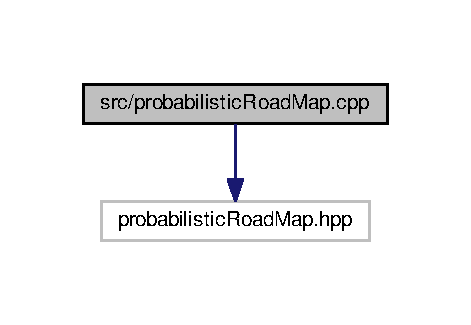
\includegraphics[width=226pt]{probabilisticRoadMap_8cpp__incl}
\end{center}
\end{figure}
\subsection*{Macros}
\begin{DoxyCompactItemize}
\item 
\#define \hyperlink{probabilisticRoadMap_8cpp_a6c116f4575d27d102053dbc576117fa4}{B\+\_\+\+O\+F\+F\+S\+ET}~0.\+06
\end{DoxyCompactItemize}
\subsection*{Functions}
\begin{DoxyCompactItemize}
\item 
bool \hyperlink{probabilisticRoadMap_8cpp_abfe1f992f72267c3dcd3295d7cc6f0a9}{is\+P\+IP} (const Point \&q\+\_\+pt, const Point \&s\+\_\+pt, const Polygon \&obj)
\item 
void \hyperlink{probabilisticRoadMap_8cpp_a69d5700b6355404bb10c95f97985c70d}{get\+Euclidian\+Dist} (const Point \&pt0, const Point \&pt1, double \&d)
\item 
bool \hyperlink{probabilisticRoadMap_8cpp_a24cb07ee59747d60da7ee436fb3e6678}{is\+Clear\+Edge} (const Point \&node0, const Point \&node1, const std\+::vector$<$ Polygon $>$ \&obstacle\+\_\+list)
\item 
bool \hyperlink{probabilisticRoadMap_8cpp_aebec67020ba69c1a3b53e656e5f845d7}{map\+\_\+cmp} (const std\+::pair$<$ Point, double $>$ \&a, const std\+::pair$<$ Point, double $>$ \&b)
\item 
void \hyperlink{probabilisticRoadMap_8cpp_a34c66507e0e4e85c289ddbf4553e06be}{get\+Min\+Distance\+Node} (const std\+::set$<$ Point $>$ \&all\+\_\+nodes\+\_\+set, const std\+::map$<$ Point, double $>$ \&distances, Point \&node\+\_\+u)
\item 
void \hyperlink{probabilisticRoadMap_8cpp_a884e484006b515130c89e5e43e258753}{get\+Graph} (const Polygon \&borders, const std\+::vector$<$ Polygon $>$ \&obstacle\+\_\+list, const std\+::vector$<$ std\+::pair$<$ int, Polygon $>$$>$ \&victim\+\_\+list, const Polygon \&gate, const Point \&robot\+\_\+bc, const int n\+\_\+pts, const int knn, std\+::map$<$ Point, std\+::vector$<$ Point $>$$>$ \&graph)
\item 
void \hyperlink{probabilisticRoadMap_8cpp_a2bc678078a49de54f4b2bb89d7b88d1e}{get\+Dijkstra\+Path} (const Point \&q\+\_\+i, const Point \&q\+\_\+f, const std\+::map$<$ Point, std\+::vector$<$ Point $>$$>$ \&graph, const std\+::vector$<$ Polygon $>$ \&obstacle\+\_\+list, std\+::vector$<$ Point $>$ \&g\+\_\+path)
\item 
void \hyperlink{probabilisticRoadMap_8cpp_ab88af9e0f07a0909c46c84a0f5d4daab}{path\+Smoother} (const std\+::vector$<$ Point $>$ \&g\+\_\+path, const std\+::vector$<$ Polygon $>$ \&obstacle\+\_\+list, std\+::vector$<$ Point $>$ \&s\+\_\+path)
\end{DoxyCompactItemize}


\subsection{Macro Definition Documentation}
\index{probabilistic\+Road\+Map.\+cpp@{probabilistic\+Road\+Map.\+cpp}!B\+\_\+\+O\+F\+F\+S\+ET@{B\+\_\+\+O\+F\+F\+S\+ET}}
\index{B\+\_\+\+O\+F\+F\+S\+ET@{B\+\_\+\+O\+F\+F\+S\+ET}!probabilistic\+Road\+Map.\+cpp@{probabilistic\+Road\+Map.\+cpp}}
\subsubsection[{\texorpdfstring{B\+\_\+\+O\+F\+F\+S\+ET}{B_OFFSET}}]{\setlength{\rightskip}{0pt plus 5cm}\#define B\+\_\+\+O\+F\+F\+S\+ET~0.\+06}\hypertarget{probabilisticRoadMap_8cpp_a6c116f4575d27d102053dbc576117fa4}{}\label{probabilisticRoadMap_8cpp_a6c116f4575d27d102053dbc576117fa4}


\subsection{Function Documentation}
\index{probabilistic\+Road\+Map.\+cpp@{probabilistic\+Road\+Map.\+cpp}!get\+Dijkstra\+Path@{get\+Dijkstra\+Path}}
\index{get\+Dijkstra\+Path@{get\+Dijkstra\+Path}!probabilistic\+Road\+Map.\+cpp@{probabilistic\+Road\+Map.\+cpp}}
\subsubsection[{\texorpdfstring{get\+Dijkstra\+Path(const Point \&q\+\_\+i, const Point \&q\+\_\+f, const std\+::map$<$ Point, std\+::vector$<$ Point $>$$>$ \&graph, const std\+::vector$<$ Polygon $>$ \&obstacle\+\_\+list, std\+::vector$<$ Point $>$ \&g\+\_\+path)}{getDijkstraPath(const Point &q_i, const Point &q_f, const std::map< Point, std::vector< Point >> &graph, const std::vector< Polygon > &obstacle_list, std::vector< Point > &g_path)}}]{\setlength{\rightskip}{0pt plus 5cm}void get\+Dijkstra\+Path (
\begin{DoxyParamCaption}
\item[{const Point \&}]{q\+\_\+i, }
\item[{const Point \&}]{q\+\_\+f, }
\item[{const std\+::map$<$ Point, std\+::vector$<$ Point $>$$>$ \&}]{graph, }
\item[{const std\+::vector$<$ Polygon $>$ \&}]{obstacle\+\_\+list, }
\item[{std\+::vector$<$ Point $>$ \&}]{g\+\_\+path}
\end{DoxyParamCaption}
)}\hypertarget{probabilisticRoadMap_8cpp_a2bc678078a49de54f4b2bb89d7b88d1e}{}\label{probabilisticRoadMap_8cpp_a2bc678078a49de54f4b2bb89d7b88d1e}
Returns, via Dijkstra algorithm, a vector of ordered nodes that determins the shortest path in the graph from the initial query point to the final query point. 
\begin{DoxyParams}[1]{Parameters}
\mbox{\tt in}  & {\em q\+\_\+i} & Query initial point. \\
\hline
\mbox{\tt in}  & {\em q\+\_\+f} & Query final point. \\
\hline
\mbox{\tt in}  & {\em graph} & Map structure defining the graph. \\
\hline
\mbox{\tt in}  & {\em obstacle\+\_\+list} & List of obstacles polygon representing the not free space. \\
\hline
\mbox{\tt out}  & {\em g\+\_\+path} & Vector of point describing the path from q\+\_\+i to q\+\_\+f. \\
\hline
\end{DoxyParams}
\index{probabilistic\+Road\+Map.\+cpp@{probabilistic\+Road\+Map.\+cpp}!get\+Euclidian\+Dist@{get\+Euclidian\+Dist}}
\index{get\+Euclidian\+Dist@{get\+Euclidian\+Dist}!probabilistic\+Road\+Map.\+cpp@{probabilistic\+Road\+Map.\+cpp}}
\subsubsection[{\texorpdfstring{get\+Euclidian\+Dist(const Point \&pt0, const Point \&pt1, double \&d)}{getEuclidianDist(const Point &pt0, const Point &pt1, double &d)}}]{\setlength{\rightskip}{0pt plus 5cm}void get\+Euclidian\+Dist (
\begin{DoxyParamCaption}
\item[{const Point \&}]{pt0, }
\item[{const Point \&}]{pt1, }
\item[{double \&}]{d}
\end{DoxyParamCaption}
)}\hypertarget{probabilisticRoadMap_8cpp_a69d5700b6355404bb10c95f97985c70d}{}\label{probabilisticRoadMap_8cpp_a69d5700b6355404bb10c95f97985c70d}
Computes the euclidean distance between two given points. 
\begin{DoxyParams}[1]{Parameters}
\mbox{\tt in}  & {\em pt0} & First point coords. \\
\hline
\mbox{\tt in}  & {\em pt1} & Second point coords. \\
\hline
\mbox{\tt out}  & {\em d} & Computed euclidean distance. \\
\hline
\end{DoxyParams}
\index{probabilistic\+Road\+Map.\+cpp@{probabilistic\+Road\+Map.\+cpp}!get\+Graph@{get\+Graph}}
\index{get\+Graph@{get\+Graph}!probabilistic\+Road\+Map.\+cpp@{probabilistic\+Road\+Map.\+cpp}}
\subsubsection[{\texorpdfstring{get\+Graph(const Polygon \&borders, const std\+::vector$<$ Polygon $>$ \&obstacle\+\_\+list, const std\+::vector$<$ std\+::pair$<$ int, Polygon $>$$>$ \&victim\+\_\+list, const Polygon \&gate, const Point \&robot\+\_\+bc, const int n\+\_\+pts, const int knn, std\+::map$<$ Point, std\+::vector$<$ Point $>$$>$ \&graph)}{getGraph(const Polygon &borders, const std::vector< Polygon > &obstacle_list, const std::vector< std::pair< int, Polygon >> &victim_list, const Polygon &gate, const Point &robot_bc, const int n_pts, const int knn, std::map< Point, std::vector< Point >> &graph)}}]{\setlength{\rightskip}{0pt plus 5cm}void get\+Graph (
\begin{DoxyParamCaption}
\item[{const Polygon \&}]{borders, }
\item[{const std\+::vector$<$ Polygon $>$ \&}]{obstacle\+\_\+list, }
\item[{const std\+::vector$<$ std\+::pair$<$ int, Polygon $>$$>$ \&}]{victim\+\_\+list, }
\item[{const Polygon \&}]{gate, }
\item[{const Point \&}]{robot\+\_\+bc, }
\item[{const int}]{n\+\_\+pts, }
\item[{const int}]{knn, }
\item[{std\+::map$<$ Point, std\+::vector$<$ Point $>$$>$ \&}]{graph}
\end{DoxyParamCaption}
)}\hypertarget{probabilisticRoadMap_8cpp_a884e484006b515130c89e5e43e258753}{}\label{probabilisticRoadMap_8cpp_a884e484006b515130c89e5e43e258753}
Returns a graph with points uniformly distributed. The graph G(\+V, E) is a key-\/value structure with verteces as keys and edges as value. 
\begin{DoxyParams}[1]{Parameters}
\mbox{\tt in}  & {\em borders} & Borders\textquotesingle{} points coord. \\
\hline
\mbox{\tt in}  & {\em obstacle\+\_\+list} & List of obstacles polygon representing the not free space. \\
\hline
\mbox{\tt in}  & {\em victim\+\_\+list} & List of victims id and polygon. \\
\hline
\mbox{\tt in}  & {\em gate} & Gate polygon. \\
\hline
\mbox{\tt in}  & {\em robot\+\_\+bc} & Robot baricenter. \\
\hline
\mbox{\tt in}  & {\em n\+\_\+pts} & Number of points to generate in the map. \\
\hline
\mbox{\tt out}  & {\em graph} & Map structure defining the graph. \\
\hline
\end{DoxyParams}
\index{probabilistic\+Road\+Map.\+cpp@{probabilistic\+Road\+Map.\+cpp}!get\+Min\+Distance\+Node@{get\+Min\+Distance\+Node}}
\index{get\+Min\+Distance\+Node@{get\+Min\+Distance\+Node}!probabilistic\+Road\+Map.\+cpp@{probabilistic\+Road\+Map.\+cpp}}
\subsubsection[{\texorpdfstring{get\+Min\+Distance\+Node(const std\+::set$<$ Point $>$ \&all\+\_\+nodes\+\_\+set, const std\+::map$<$ Point, double $>$ \&distances, Point \&node\+\_\+u)}{getMinDistanceNode(const std::set< Point > &all_nodes_set, const std::map< Point, double > &distances, Point &node_u)}}]{\setlength{\rightskip}{0pt plus 5cm}void get\+Min\+Distance\+Node (
\begin{DoxyParamCaption}
\item[{const std\+::set$<$ Point $>$ \&}]{all\+\_\+nodes\+\_\+set, }
\item[{const std\+::map$<$ Point, double $>$ \&}]{distances, }
\item[{Point \&}]{node\+\_\+u}
\end{DoxyParamCaption}
)}\hypertarget{probabilisticRoadMap_8cpp_a34c66507e0e4e85c289ddbf4553e06be}{}\label{probabilisticRoadMap_8cpp_a34c66507e0e4e85c289ddbf4553e06be}
Given the a set of nodes and the distances map of Dijkstra algorithm, it provides the node with minimum distance. 
\begin{DoxyParams}[1]{Parameters}
\mbox{\tt in}  & {\em all\+\_\+nodes\+\_\+set} & Set with all nodes that need to be sorted. \\
\hline
\mbox{\tt in}  & {\em distances} & Map of distances\+: distances\mbox{[}u\mbox{]} = n -\/$>$ distance n from q\+\_\+i to u. \\
\hline
\mbox{\tt out}  & {\em node\+\_\+u} & Node in distances map with minimum distance. \\
\hline
\end{DoxyParams}
\index{probabilistic\+Road\+Map.\+cpp@{probabilistic\+Road\+Map.\+cpp}!is\+Clear\+Edge@{is\+Clear\+Edge}}
\index{is\+Clear\+Edge@{is\+Clear\+Edge}!probabilistic\+Road\+Map.\+cpp@{probabilistic\+Road\+Map.\+cpp}}
\subsubsection[{\texorpdfstring{is\+Clear\+Edge(const Point \&node0, const Point \&node1, const std\+::vector$<$ Polygon $>$ \&obstacle\+\_\+list)}{isClearEdge(const Point &node0, const Point &node1, const std::vector< Polygon > &obstacle_list)}}]{\setlength{\rightskip}{0pt plus 5cm}bool is\+Clear\+Edge (
\begin{DoxyParamCaption}
\item[{const Point \&}]{node0, }
\item[{const Point \&}]{node1, }
\item[{const std\+::vector$<$ Polygon $>$ \&}]{obstacle\+\_\+list}
\end{DoxyParamCaption}
)}\hypertarget{probabilisticRoadMap_8cpp_a24cb07ee59747d60da7ee436fb3e6678}{}\label{probabilisticRoadMap_8cpp_a24cb07ee59747d60da7ee436fb3e6678}
Given two graph\textquotesingle{}s edeges it returns true if they do not collide with any of the provided obstacles, false otherwise. 
\begin{DoxyParams}[1]{Parameters}
\mbox{\tt in}  & {\em node0} & First graph\textquotesingle{}s node. \\
\hline
\mbox{\tt in}  & {\em node0} & Second graph\textquotesingle{}s node. \\
\hline
\mbox{\tt in}  & {\em obstacle\+\_\+list} & List of Polygon obstacles. \\
\hline
\end{DoxyParams}
\begin{DoxyReturn}{Returns}
\mbox{[}bool\mbox{]} Bool true if graph\textquotesingle{}s edge do not collide with any obstacle, false otherwise. 
\end{DoxyReturn}
\index{probabilistic\+Road\+Map.\+cpp@{probabilistic\+Road\+Map.\+cpp}!is\+P\+IP@{is\+P\+IP}}
\index{is\+P\+IP@{is\+P\+IP}!probabilistic\+Road\+Map.\+cpp@{probabilistic\+Road\+Map.\+cpp}}
\subsubsection[{\texorpdfstring{is\+P\+I\+P(const Point \&q\+\_\+pt, const Point \&s\+\_\+pt, const Polygon \&obj)}{isPIP(const Point &q_pt, const Point &s_pt, const Polygon &obj)}}]{\setlength{\rightskip}{0pt plus 5cm}bool is\+P\+IP (
\begin{DoxyParamCaption}
\item[{const Point \&}]{q\+\_\+pt, }
\item[{const Point \&}]{s\+\_\+pt, }
\item[{const Polygon \&}]{obj}
\end{DoxyParamCaption}
)}\hypertarget{probabilisticRoadMap_8cpp_abfe1f992f72267c3dcd3295d7cc6f0a9}{}\label{probabilisticRoadMap_8cpp_abfe1f992f72267c3dcd3295d7cc6f0a9}
Returns true if the point is internal to a given polygon. It verifies the condition of the query point via ray-\/casting algorithm. (P\+IP -\/ Point In Polygon). 
\begin{DoxyParams}[1]{Parameters}
\mbox{\tt in}  & {\em q\+\_\+pt} & Query point coordinates. \\
\hline
\mbox{\tt in}  & {\em s\+\_\+pt} & Safe external point coordinates. \\
\hline
\mbox{\tt in}  & {\em obj} & Polygon object. \\
\hline
\end{DoxyParams}
\begin{DoxyReturn}{Returns}
\mbox{[}bool\mbox{]} Bool true if the query point is internal, false otherwise. 
\end{DoxyReturn}
\index{probabilistic\+Road\+Map.\+cpp@{probabilistic\+Road\+Map.\+cpp}!map\+\_\+cmp@{map\+\_\+cmp}}
\index{map\+\_\+cmp@{map\+\_\+cmp}!probabilistic\+Road\+Map.\+cpp@{probabilistic\+Road\+Map.\+cpp}}
\subsubsection[{\texorpdfstring{map\+\_\+cmp(const std\+::pair$<$ Point, double $>$ \&a, const std\+::pair$<$ Point, double $>$ \&b)}{map_cmp(const std::pair< Point, double > &a, const std::pair< Point, double > &b)}}]{\setlength{\rightskip}{0pt plus 5cm}bool map\+\_\+cmp (
\begin{DoxyParamCaption}
\item[{const std\+::pair$<$ Point, double $>$ \&}]{a, }
\item[{const std\+::pair$<$ Point, double $>$ \&}]{b}
\end{DoxyParamCaption}
)}\hypertarget{probabilisticRoadMap_8cpp_aebec67020ba69c1a3b53e656e5f845d7}{}\label{probabilisticRoadMap_8cpp_aebec67020ba69c1a3b53e656e5f845d7}
Returns true if the second element of the first pair is less than the second element of the second pair. 
\begin{DoxyParams}[1]{Parameters}
\mbox{\tt in}  & {\em a} & First pair. \\
\hline
\mbox{\tt in}  & {\em b} & Second pair. \\
\hline
\end{DoxyParams}
\begin{DoxyReturn}{Returns}
\mbox{[}bool\mbox{]} Bool true if a second element is less than b second element, false otherwise. 
\end{DoxyReturn}
\index{probabilistic\+Road\+Map.\+cpp@{probabilistic\+Road\+Map.\+cpp}!path\+Smoother@{path\+Smoother}}
\index{path\+Smoother@{path\+Smoother}!probabilistic\+Road\+Map.\+cpp@{probabilistic\+Road\+Map.\+cpp}}
\subsubsection[{\texorpdfstring{path\+Smoother(const std\+::vector$<$ Point $>$ \&g\+\_\+path, const std\+::vector$<$ Polygon $>$ \&obstacle\+\_\+list, std\+::vector$<$ Point $>$ \&s\+\_\+path)}{pathSmoother(const std::vector< Point > &g_path, const std::vector< Polygon > &obstacle_list, std::vector< Point > &s_path)}}]{\setlength{\rightskip}{0pt plus 5cm}void path\+Smoother (
\begin{DoxyParamCaption}
\item[{const std\+::vector$<$ Point $>$ \&}]{g\+\_\+path, }
\item[{const std\+::vector$<$ Polygon $>$ \&}]{obstacle\+\_\+list, }
\item[{std\+::vector$<$ Point $>$ \&}]{s\+\_\+path}
\end{DoxyParamCaption}
)}\hypertarget{probabilisticRoadMap_8cpp_ab88af9e0f07a0909c46c84a0f5d4daab}{}\label{probabilisticRoadMap_8cpp_ab88af9e0f07a0909c46c84a0f5d4daab}
Given a graph path, it provides a smoothed version. 
\begin{DoxyParams}[1]{Parameters}
\mbox{\tt in}  & {\em g\+\_\+path} & Graph path found with Dijkstra (at least 3 points). \\
\hline
\mbox{\tt in}  & {\em obstacle\+\_\+list} & List of obstacles polygon representing the not free space. \\
\hline
\mbox{\tt out}  & {\em s\+\_\+path} & Smoothed path. \\
\hline
\end{DoxyParams}

\hypertarget{student__interface_8cpp}{}\section{src/student\+\_\+interface.cpp File Reference}
\label{student__interface_8cpp}\index{src/student\+\_\+interface.\+cpp@{src/student\+\_\+interface.\+cpp}}
{\ttfamily \#include \char`\"{}student\+\_\+image\+\_\+elab\+\_\+interface.\+hpp\char`\"{}}\\*
{\ttfamily \#include \char`\"{}student\+\_\+planning\+\_\+interface.\+hpp\char`\"{}}\\*
{\ttfamily \#include \char`\"{}image\+Manager.\+hpp\char`\"{}}\\*
{\ttfamily \#include \char`\"{}extrinsic\+Calib.\+hpp\char`\"{}}\\*
{\ttfamily \#include \char`\"{}map\+Processing.\+hpp\char`\"{}}\\*
{\ttfamily \#include \char`\"{}path\+Planning.\+hpp\char`\"{}}\\*
{\ttfamily \#include $<$opencv2/opencv.\+hpp$>$}\\*
Include dependency graph for student\+\_\+interface.\+cpp\+:\nopagebreak
\begin{figure}[H]
\begin{center}
\leavevmode
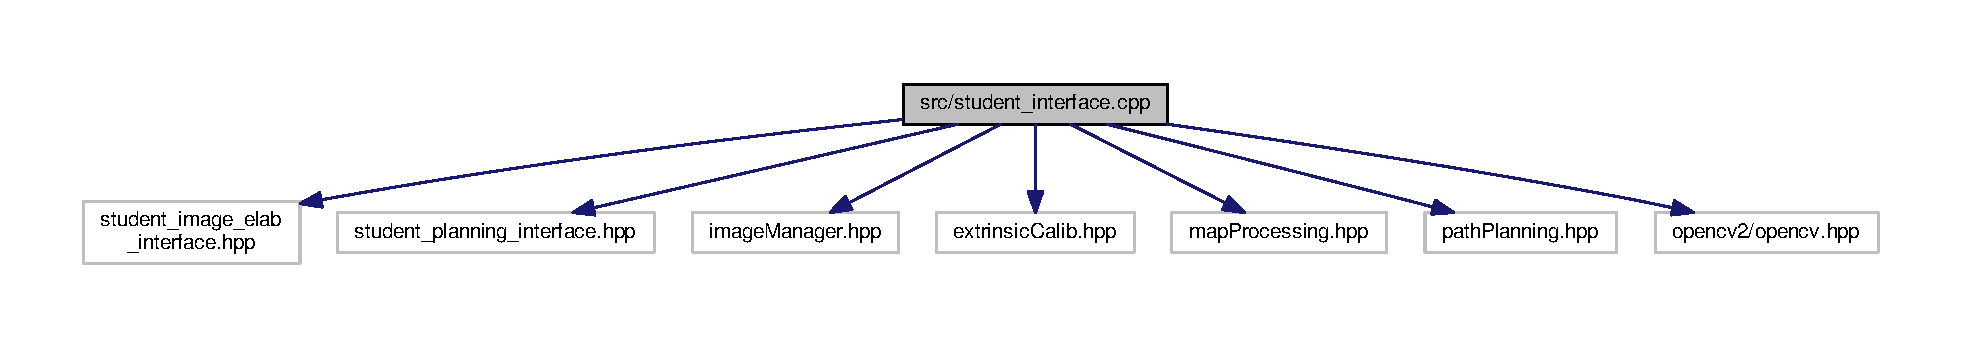
\includegraphics[width=350pt]{student__interface_8cpp__incl}
\end{center}
\end{figure}
\subsection*{Namespaces}
\begin{DoxyCompactItemize}
\item 
 \hyperlink{namespacestudent}{student}
\end{DoxyCompactItemize}
\subsection*{Functions}
\begin{DoxyCompactItemize}
\item 
void \hyperlink{namespacestudent_a3117c968a47bf95f86bdb813a3b64e56}{student\+::load\+Image} (cv\+::\+Mat \&img\+\_\+out, const std\+::string \&config\+\_\+folder)
\item 
void \hyperlink{namespacestudent_a3b726e7af03a643c06dcde23057a82ea}{student\+::generic\+Image\+Listener} (const cv\+::\+Mat \&img\+\_\+in, std\+::string topic, const std\+::string \&config\+\_\+folder)
\item 
bool \hyperlink{namespacestudent_a6103f938ce28f8820c48c089d5f95098}{student\+::extrinsic\+Calib} (const cv\+::\+Mat \&img\+\_\+in, std\+::vector$<$ cv\+::\+Point3f $>$ object\+\_\+points, const cv\+::\+Mat \&camera\+\_\+matrix, cv\+::\+Mat \&rvec, cv\+::\+Mat \&tvec, const std\+::string \&config\+\_\+folder)
\item 
void \hyperlink{namespacestudent_aceb2a29362b8223a9d3601d9496e1c98}{student\+::image\+Undistort} (const cv\+::\+Mat \&img\+\_\+in, cv\+::\+Mat \&img\+\_\+out, const cv\+::\+Mat \&cam\+\_\+matrix, const cv\+::\+Mat \&dist\+\_\+coeffs, const std\+::string \&config\+\_\+folder)
\item 
void \hyperlink{namespacestudent_a528d33658d0d4d982a46f18b7abb4a70}{student\+::find\+Plane\+Transform} (const cv\+::\+Mat \&cam\+\_\+matrix, const cv\+::\+Mat \&rvec, const cv\+::\+Mat \&tvec, const std\+::vector$<$ cv\+::\+Point3f $>$ \&object\+\_\+points\+\_\+plane, const std\+::vector$<$ cv\+::\+Point2f $>$ \&dest\+\_\+image\+\_\+points\+\_\+plane, cv\+::\+Mat \&plane\+\_\+transf, const std\+::string \&config\+\_\+folder)
\item 
void \hyperlink{namespacestudent_a6b8caf348979f55e58a75193233c219d}{student\+::unwarp} (const cv\+::\+Mat \&img\+\_\+in, cv\+::\+Mat \&img\+\_\+out, const cv\+::\+Mat \&transf, const std\+::string \&config\+\_\+folder)
\item 
bool \hyperlink{namespacestudent_a684c71c41ce1327ab90152b661ee1e8a}{student\+::process\+Map} (const cv\+::\+Mat \&img\+\_\+in, const double scale, std\+::vector$<$ Polygon $>$ \&obstacles\+\_\+list, std\+::vector$<$ std\+::pair$<$ int, Polygon $>$$>$ \&victims\+\_\+list, Polygon \&gate, const std\+::string \&config\+\_\+folder)
\item 
bool \hyperlink{namespacestudent_afd56b779672a672e15ac45dc927b8a6b}{student\+::find\+Robot} (const cv\+::\+Mat \&img\+\_\+in, const double scale, Polygon \&triangle, double \&x, double \&y, double \&theta, const std\+::string \&config\+\_\+folder)
\item 
bool \hyperlink{namespacestudent_acfe62076a49d23bb083f2f880fd24c77}{student\+::plan\+Path} (const Polygon \&borders, const std\+::vector$<$ Polygon $>$ \&obstacle\+\_\+list, const std\+::vector$<$ std\+::pair$<$ int, Polygon $>$$>$ \&victim\+\_\+list, const Polygon \&gate, const float x, const float y, const float theta, Path \&path, const std\+::string \&config\+\_\+folder)
\end{DoxyCompactItemize}

\hypertarget{utils_8cpp}{}\section{src/utils.cpp File Reference}
\label{utils_8cpp}\index{src/utils.\+cpp@{src/utils.\+cpp}}
{\ttfamily \#include \char`\"{}utils.\+hpp\char`\"{}}\\*
Include dependency graph for utils.\+cpp\+:\nopagebreak
\begin{figure}[H]
\begin{center}
\leavevmode
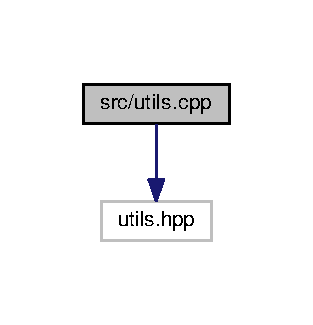
\includegraphics[width=150pt]{utils_8cpp__incl}
\end{center}
\end{figure}
\subsection*{Functions}
\begin{DoxyCompactItemize}
\item 
void \hyperlink{utils_8cpp_a3ae4495b90e30e512e3a8c6cf7b9f671}{get\+Baricenter} (const Polygon \&obj, Point \&baricenter)
\item 
void \hyperlink{utils_8cpp_afe0eaeeed2847a469106dbde975ac757}{get\+Baricenter} (const Polygon \&obj, double \&x, double \&y)
\end{DoxyCompactItemize}


\subsection{Function Documentation}
\index{utils.\+cpp@{utils.\+cpp}!get\+Baricenter@{get\+Baricenter}}
\index{get\+Baricenter@{get\+Baricenter}!utils.\+cpp@{utils.\+cpp}}
\subsubsection[{\texorpdfstring{get\+Baricenter(const Polygon \&obj, Point \&baricenter)}{getBaricenter(const Polygon &obj, Point &baricenter)}}]{\setlength{\rightskip}{0pt plus 5cm}void get\+Baricenter (
\begin{DoxyParamCaption}
\item[{const Polygon \&}]{obj, }
\item[{Point \&}]{baricenter}
\end{DoxyParamCaption}
)}\hypertarget{utils_8cpp_a3ae4495b90e30e512e3a8c6cf7b9f671}{}\label{utils_8cpp_a3ae4495b90e30e512e3a8c6cf7b9f671}
Retrieves the baricenter of the provided polygon. 
\begin{DoxyParams}[1]{Parameters}
\mbox{\tt in}  & {\em obj} & Polygon with unknown baricenter. \\
\hline
\mbox{\tt out}  & {\em baricenter} & Baricenter point. \\
\hline
\end{DoxyParams}
\index{utils.\+cpp@{utils.\+cpp}!get\+Baricenter@{get\+Baricenter}}
\index{get\+Baricenter@{get\+Baricenter}!utils.\+cpp@{utils.\+cpp}}
\subsubsection[{\texorpdfstring{get\+Baricenter(const Polygon \&obj, double \&x, double \&y)}{getBaricenter(const Polygon &obj, double &x, double &y)}}]{\setlength{\rightskip}{0pt plus 5cm}void get\+Baricenter (
\begin{DoxyParamCaption}
\item[{const Polygon \&}]{obj, }
\item[{double \&}]{x, }
\item[{double \&}]{y}
\end{DoxyParamCaption}
)}\hypertarget{utils_8cpp_afe0eaeeed2847a469106dbde975ac757}{}\label{utils_8cpp_afe0eaeeed2847a469106dbde975ac757}
Retrieves the baricenter of the provided polygon. 
\begin{DoxyParams}[1]{Parameters}
\mbox{\tt in}  & {\em obj} & Polygon with unknown baricenter. \\
\hline
\mbox{\tt out}  & {\em x} & Baricenter x coord. \\
\hline
\mbox{\tt out}  & {\em y} & Baricenter y coord. \\
\hline
\end{DoxyParams}

%--- End generated contents ---

% Index
\backmatter
\newpage
\phantomsection
\clearemptydoublepage
\addcontentsline{toc}{chapter}{Index}
\printindex

\end{document}
